\providecommand{\toplevelprefix}{../..}  % necessary for subfile bibliography + figures compilation to work, do not move this after documentclass

\documentclass[../../book-main.tex]{subfiles}
\usepackage[UTF8]{ctex}
\graphicspath{{\subfix{../..}}}

\begin{document}

\chapter{一致性与自洽性表示}
\label{ch:consistent}\label{ch:autoencoding}
\label{ch:self-consistent}\label{ch:closed-loop}

\begin{quote}
\hfill  ``{\em 凡事应力求简单,但不应过于简单}。''

$~$\hfill -- 阿尔伯特·爱因斯坦
\end{quote}

% \begin{quote}
%   \hfill  ``{\em It has been obvious since the 1980s that
%     backpropagation through deep autoencoders would be very effective
%     for nonlinear dimensionality reduction, provided that computers
%     were fast enough, data sets were big enough, and the initial
%     weights were close enough to a good solution. All three conditions
%   are now satisfied}.''
%   \hfill  ``{\em 自20世纪80年代以来,一个显而易见的事实是,只要计算机足够快,数据集足够大,并且初始权重足够接近一个好的解,那么通过深度自编码器进行反向传播对于非线性降维将非常有效。如今,这三个条件都已满足}。''

%   $~$\hfill -- Geoffrey Hinton and Ruslan  Salakhutdinov, 2006
% \end{quote}

\vspace{5mm}


在前面的章节中,我们已经阐明了一个基本事实:学习的根本目标是学习一个具有低维支撑的数据分布,并将其转换为一个紧凑且结构化的表示。这种表示揭示了数据分布内在的低维结构,并为后续的分类和生成等任务提供了便利。

学习这种分布的良好表示的一个基本方法是通过{\em 压缩}。为了使压缩的目标可度量和可计算,可以通过学习一种编码方案来明确实现,该方案旨在最小化编码率(熵)或最大化信息增益(编码率降低)。在此背景下,深度神经网络的基本作用是实现某种迭代优化算法,该算法根据这些度量逐步优化所学到的表示:
\begin{equation}
  f\colon \X
  \xrightarrow{\hspace{1mm} f^0 \hspace{1mm}} \Z^0 \rightarrow \cdots
  \rightarrow \Z^\ell \xrightarrow{\hspace{1mm} f^\ell \hspace{1mm}}
  \Z^{\ell+1} \rightarrow  \cdots \to \Z^L = \Z.
\end{equation}
在上一章中,我们已经展示了几乎所有流行的深度网络(ResNet、CNN 和 Transformer)的主要架构特性都可以从这个角度推导和解释。

然而,当我们试图通过优化实现某个目标时,并不能保证通过增量优化最终找到的解 $\Z$ 就是正确的解。事实上,即使优化过程成功找到了全局最优解 $\Z^*$,也无法保证该解对应于数据分布的完整表示。\footnote{这可能由多种原因导致:例如,可用于学习分布的数据可能不充分,或者优化问题的公式未能考虑一些额外的约束或条件。}因此,一个悬而未决的问题是,我们如何确保所学到的数据分布表示是正确或足够好的?

当然,验证这一点的唯一方法是看是否存在一个解码映射(比如 $g$),能够将所学到的表示解码,以足够好地再现原始数据(分布):
\begin{equation}
  \X
  \xrightarrow{\hspace{1mm} \mathcal{E} = f \hspace{1mm}} \Z
  \xrightarrow{\hspace{1mm} \mathcal{D} = g \hspace{1mm}} \hat{\X}
\end{equation}
根据某种相似性度量:
\begin{equation}
  d(\X, \hat \X).
\end{equation}
这就引出了{\em 一致性表示}的概念。正如我们在第 \ref{ch:intro} 章中简要提到的(见图 \ref{fig:autoencoder}),集成了编码和解码过程的{\em 自编码}是学习这种表示的自然框架。我们已经在第 \ref{ch:classic} 章中研究了一些重要的特例。在本章的第 \ref{sec:consistent-representation} 节和第 \ref{sec:NLPCA} 节中,我们将研究如何通过强制 $\X$ 和 $\hat \X$ 之间的一致性,将自编码扩展到更一般的分布类别。

在许多实际和自然的学习场景中,比较数据 $\X$ 和 $\hat \X$ 的分布可能很困难,甚至不可能。我们只剩下唯一的选择,即在编码器 $f$ 下,比较学习到的特征 $\Z$ 与其像 $\hat \Z$:
\begin{equation}
 \X
\xrightarrow{\hspace{1mm} \mathcal{E} = f \hspace{1mm}} \Z  \xrightarrow{\hspace{1mm} \mathcal{D} = g \hspace{1mm}} \hat{\X} \xrightarrow{\hspace{1mm} \mathcal{E} = f \hspace{1mm}} \hat \Z?
% \label{eqn:closed-autoencoding}
\end{equation}
这就引出了{\em 自洽性表示}的概念。在第 \ref{sec:self-consistency} 节和第 \ref{sec:closed-loop-transcription} 节中,我们将研究何时以及如何仅通过一个闭环转录框架,通过强制 $\Z$ 和 $\hat \Z$ 之间的自洽性来学习一致性表示。

此外,在许多实际和自然的学习场景中,我们通常无法一次性获得数据分布的足够样本。例如,动物和人类通过一生中不断接收增量的观察来发展其视觉记忆。在第 \ref{sec:continuous} 节中,我们将研究如何扩展闭环转录框架,以在{\em 持续学习}的设置中学习自洽性表示。

当然,我们之所以想要识别数据分布中的低维结构并找到一个好的表示,一个根本的动机是为了方便将数据用于各种智能任务,如分类、补全和预测。因此,最终得到的联合表示 $(\x, \z)$ 必须以最适合这些任务的方式进行结构化。在下一章中,我们将看到如何结构化所学到的表示,以促进条件补全或生成任务。

\section{学习一致性表示}\label{sec:consistent-representation}
%\yima{Rewrite this to state the mathematical problem clearly,
% including assumptions (e.g. sufficiency) and objectives. Discuss
% approximations or variants of the objective that are computable and
% implementable.}

这里我们给出一致性表示的正式定义,它与自编码的概念密切相关。%\yima{Maybe we
% want to separate definitions for the two types of consistency:
% Sample wise versus distribution wise.}
\begin{definition}[一致性表示]\label{def:bidirectional_rep}
  给定数据 \(\vX\),一个\textit{一致性表示}是一对函数 \((f \colon \cX \to \cZ, g \colon \cZ \to \cX)\),使得\textit{特征} \(\vZ = f(\vX)\) 是紧凑且结构化的,并且\textit{自编码} \[\hat{\vX} \doteq g(\vZ)
  = g(f(\vZ))\] 根据以下两种度量之一与 \(\vX\) \textit{接近}:
  \begin{enumerate}
    \item 如果 \(\vX \approx \hat{\vX}\) 在某种范数下以高概率成立,我们称其为\textit{样本级}一致。
    \item 如果 \(\Law(\vX) \approx \Law(\hat{\vX})\),我们称该表示是\textit{分布级}一致的。
  \end{enumerate}
\end{definition}
%\sdb{Connected to perception vs.\ distortion.}

敏锐的读者可能已经注意到,如果我们不对所寻求的表示 $\Z$ 施加某些要求,上述问题会有一个平凡解:我们可以简单地选择函数 $f$ 和 $g$ 为恒等映射!因此,寻求自编码的真正目的是试图确保所获得的 $\Z$ 比 $\X$ 更紧凑、更结构化。首先,为了紧凑性,$\Z$ 应该更好地揭示 $\X$ 的内在低维性。因此,该表示应最大化某种信息增益,例如,用在 \Cref{subsec:MCR2} 中介绍的编码率降低来衡量:
\begin{equation}
  \Delta R_{\epsilon}(\Z)
\end{equation}
其次,学习数据分布的良好表示的主要目的是为了方便利用其分布的低维性来完成任务。因此,$\Z$ 的分布应该更具结构性。例如,$\Z$ 的分布是分段线性的或高斯的,其分量在很大程度上是不相关的或独立的等等。这些独立的分量可以代表不同的簇或类别,也可以很容易地用作解码相应数据 $\x$ 的条件。

根据一致性表示的定义,它要求表示 $\Z$ 足以在一定精度上恢复原始数据分布 $\X$。对于样本级一致性,一个典型的选择是最小化期望重构误差:
\begin{equation}
  d(\X, \hat \X) = \mathbb{E}[\|\X - \hat\X\|_2^2].
\end{equation}
对于分布上的一致性,一个典型的选择是最小化某种分布距离,如 KL 散度\footnote{注意,对于没有共同支撑的分布(这对于退化分布是典型的),KL 散度甚至可能没有明确定义。事实上,许多分布学习文献正试图通过用一些定义良好且可高效计算的东西来替换或近似它,以解决这一技术难题。}:
\begin{equation}
  d(\X, \hat \X) = \mathcal{D}_{KL}(\X\|\hat\X).
\end{equation}

因此,撇开计算不谈,当我们为数据分布 $\X$ 寻求一个好的自编码时,概念上我们试图找到一个编码器 $f$ 和一个解码器 $g$,使得
\begin{equation}
  \min_{f, g} - \Delta R_{\epsilon}(\Z) + d(\X, \hat \X).
  \label{eqn:autoencode-objective-ch5}
\end{equation}
%\sdb{Maximize $\Delta R$?}
在本章的其余部分,我们将研究如何在不同条件下解决这类自编码问题,从简单和理想的情况到越来越具有挑战性和现实性的情况。

%\section{From Linear to Nonlinear Autoencoding}\label{sec:NLPCA}
%\yima{How to ensure the representation is compact and structured,
% say linear or piecewise linear, or informative? Classical
% autoencoders do not explicitly impose such... Incremental
% flattening transformation, particularly
% \href{https://arxiv.org/abs/2305.01777}{nonlinear manifold
% flattening and reconstruction}. This is an example of consistency
% in sample-wise reconstruction.}

\subsection{通过 PCA 实现线性自编码}
根据 \cite{Baldi2011},术语“自编码器”最早由 Hinton 和 Rumelhart \cite{Rumelhart1986} 提出,以便通过反向传播(BP)以自监督的方式学习深度表示——重构原始数据就是自监督任务。

然而,寻求紧凑且一致的表示这一概念早已植根于许多经典研究中。正如我们在第 \ref{ch:classic} 章中已经看到的,经典的 PCA、ICA 和稀疏字典学习都有着相似的目标。唯一的区别是,当底层数据分布很简单(线性和独立的)时,编码或解码映射变得易于表示和学习:它们不需要很深,并且通常可以以闭式形式或通过显式算法计算。

看看我们定义的一致性概念在 PCA 这个简单案例中是如何体现的,是很有启发性的:在这里,一致的编码和解码映射由一个单层线性变换给出:
\begin{equation}
  \X \xrightarrow{\hspace{2mm} \mathcal{E} = \vU^\top \hspace{2mm}}
  \Z \xrightarrow{\hspace{2mm} \mathcal{D} = \vU \hspace{2mm}}   \hat{\X},
  \label{eqn:autoencoding-PCA-2}
\end{equation}
其中 $\vU \in \mathbb{R}^{D\times d}$,通常 $d\ll D$。因此,$\vU^\top$ 表示从高维空间 $\mathbb{R}^{D}$ 到低维空间 $\mathbb{R}^{d}$ 的投影,如图 \ref{fig:AE} 所示。
\begin{figure}
  \centering 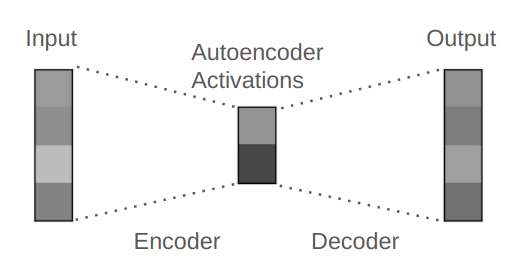
\includegraphics[width=0.5\linewidth]{\toplevelprefix/chapters/chapter5/figs/autoencoder.png}
  \caption{一个典型的自编码器(如 PCA)的示意图,它为高维数据 $\vx$ 寻求一个低维表示 $\bm{z}$。}
  \label{fig:AE}
\end{figure}

正如我们在第 \ref{ch:classic} 章中看到的,当 $\vx$ 的分布确实支撑在一个低维子空间 $\vU_o$ 上时,由 $\cE$ 产生的表示 $\vz$ 的紧凑性是正确估计(并强制执行)该子空间维度的直接结果。最后,回想一下,对重构准则进行梯度下降恰好可以得到这些样本级一致的映射:实际上,当表示的维度足够大时,问题
\begin{equation}\label{eq:pca-reconstruction-ch5}
  \min_{\vU^\top \vU = \vI}\, \bE_{\vx}\left[\norm*{\vx
  - \vU\vU^\top \vx}_2^2\right]
\end{equation}
的最优解恰好与 $\vU_o$ 一致。在这种情况下,我们免费获得了样本级一致性,因为这保证了 $\vU_o\vU_o^\top \vx = \vx$。
请注意,在 PCA 的情况下,\eqref{eqn:autoencode-objective-ch5} 中的编码率降低项变得无效,因为对所寻求的表示 $\Z$ 的正则化是显式的:它跨越了整个低维子空间\footnote{在这种情况下,可以看作 $\Delta R = 0$。}。

\paragraph{在线 PCA。} 请注意,在上述构造中,用于编码和解码的线性变换 $\vU$ 是事先从所有输入数据中“离线”计算的。一个问题是,这个变换是否可以在输入数据按顺序到来时“在线”学习?这个问题由 Oja 在 1982 年的工作 \cite{Oja1982SimplifiedNM} 回答了。
\begin{example}[PCA 的归一化赫布学习方案] 考虑一系列独立同分布的随机向量 $\x_1, \ldots, \x_i, \ldots \in
  \mathbb{R}^n$,其协方差为 $\boldsymbol{\Sigma} \in
  \mathbb{R}^{n\times n}$。令 $\vu_0 \in \mathbb{R}^n$,并定义输入向量 $\x_i$ 对权重向量 $\vu_i$ 的响应为其内积:
  \begin{equation}
    \eta_i = \vu_i^T \x_i
  \end{equation}
  我们根据以下方案更新权重向量:
  \begin{equation}
    \vu_{i+1} = \frac{\vu_i + \gamma \eta_i \x_i}{\|\vu_i + \gamma
    \eta_i \x_i\|}
    \label{eqn:Hebbian}
  \end{equation}
  其中 $\gamma >0$ 是某个小的增益。这个更新方案可以看作是一个归一化的赫布方案,其中如果输入 $\x$ 和输出 $\eta$(的乘积)都很强,神经元之间的连接权重就会变强。可以认为权重向量 $\vu$ 是基于输出 $\eta$ 的某种形式的反馈而“学习”到的。
  那么,在合理的假设下,Oja \cite{Oja1982SimplifiedNM} 已经证明 $\vu_i$ 收敛到与 $\boldsymbol{\Sigma}$ 的大特征值相关联的特征向量。
\end{example}

归一化的赫布方案 \eqref{eqn:Hebbian} 可以被解释为问题 \eqref{eq:pca-reconstruction-ch5} 目标函数上的\textit{随机}投影梯度下降方案的一阶近似(批量大小为 1,$\vU$ 的列数为 1),只要 $\norm{\vu}_2 = 1$,这一点由 \eqref{eqn:Hebbian} 中的投影操作来维持。
值得记住它的存在,这既是使用随机梯度方法优化像 \eqref{eq:pca-reconstruction-ch5} 这样的重构成本的正确性证明,也因为它暗示了\textit{比(端到端)反向传播更简单的算法可以成功学习一致的自编码器}。

\begin{figure}
  \centering
  % \includegraphics[width=12cm]{interpolate.jpg}
  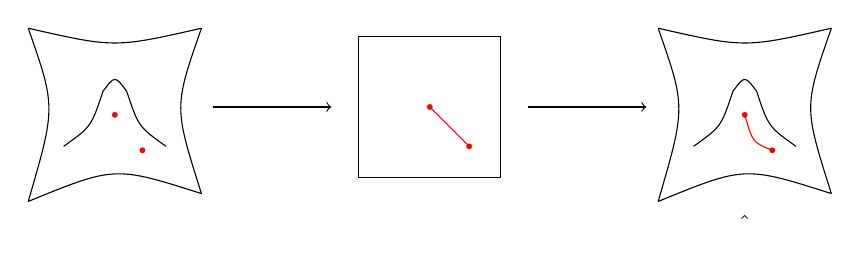
\begin{tikzpicture}
    \draw (-0.1, -0.2) .. controls (1, 0.25) .. (2.1, -0.1);
    \draw (2.1, -0.1) .. controls (1.75, 1) .. (2.1, 2);
    \draw (2.1, 2) .. controls (1, 1.75) .. (-0.1, 2);
    \draw (-0.1, 2) .. controls (0.25, 1) .. (-0.1, -0.2);

    \draw (0.35, 0.5) .. controls (0.7, 0.75) .. (0.85, 1.2);
    \draw (0.85, 1.2) .. controls (1.0, 1.4) .. (1.15, 1.2);
    \draw (1.15, 1.2) .. controls (1.3, 0.75) .. (1.65, 0.5);

    \node[fill, red, circle, inner sep=0.75pt] at (1, 0.9) {};
    \node[fill, red, circle, inner sep=0.75pt] at (1.35, 0.45) {};

    \node at (1, -0.5) {\(\x\)};

    \draw[->] (2.25, 1) -- (3.75, 1);
    \node at (3, 1.25) {\(\fl\)};

    \draw (4.1, 0.1) -- (5.9, 0.1);
    \draw (5.9, 0.1) -- (5.9, 1.9);
    \draw (5.9, 1.9) -- (4.1, 1.9);
    \draw (4.1, 1.9) -- (4.1, 0.1);

    \node[fill, red, circle, inner sep=0.75pt] at (5, 1) {};
    \node[fill, red, circle, inner sep=0.75pt] at (5.5, 0.5) {};

    \draw[red] (5, 1) -- (5.5, 0.5);

    \node at (5, -0.5) {\(\z\)};

    \draw[->] (6.25, 1) -- (7.75, 1);
    \node at (7, 1.25) {\(\re\)};

    \draw (7.9, -0.2) .. controls (9, 0.25) .. (10.1, -0.1);
    \draw (10.1, -0.1) .. controls (9.75, 1) .. (10.1, 2);
    \draw (10.1, 2) .. controls (9, 1.75) .. (7.9, 2);
    \draw (7.9, 2) .. controls (8.25, 1) .. (7.9, -0.2);

    \draw (8.35, 0.5) .. controls (8.7, 0.75) .. (8.85, 1.2);
    \draw (8.85, 1.2) .. controls (9.0, 1.4) .. (9.15, 1.2);
    \draw (9.15, 1.2) .. controls (9.3, 0.75) .. (9.65, 0.5);

    \node[fill, red, circle, inner sep=0.75pt] at (9, 0.9) {};
    \node[fill, red, circle, inner sep=0.75pt] at (9.35, 0.45) {};

    \draw[red] (9, 0.9) .. controls (9.1, 0.55) .. (9.35, 0.45);

    \node at (9, -0.5) {\(\hat{\x}\)};
  \end{tikzpicture}
  \caption{通过流形展平在维度 \(d = 2\) 的 \(\R^{3}\) 流形上进行插值的示意图。为了在数据流形上对两点进行插值,通过展平映射 \(\fl\) 将它们映射到展平空间,取它们的凸插值,然后通过重构映射 \(\re\) 将它们映射回数据流形。}
  \label{fig:idealized_interpolation}
\end{figure}

\subsection{非线性 PCA 与自编码}\label{sub:nonlinear-pca}\label{sec:NLPCA}
当然,当我们处理更复杂的分布,其潜在的低维结构可能是非线性时,我们应该预料到事情将不再那么简单。

\paragraph{非线性子流形上的数据。} 因此,为了超越 PCA 处理的线性结构,我们可以假设数据分布位于一个(光滑的)子流形 $\mathcal{M}$ 上。该子流形的内在维度(比如 $d$)通常远低于环境空间 $\mathbb{R}^D$ 的维度。从这个几何角度来看,我们通常希望找到一个非线性映射 $f$,使得得到的流形 $f(\mathcal{M})$ 被展平,如图 \ref{fig:idealized_interpolation} 所示的例子。得到的特征 $\vz$-空间通常比 $\vx$-空间更紧凑(维度更低),并且流形是平坦的。
从统计学的角度来看(这与几何角度互补,但通常是不同的),我们可能还希望确保 $\cM$ 上的数据分布被映射到 $\vz$-空间中一个足够规则的分布,比如高斯分布或均匀分布(具有非常低维的支撑)。这两个性质确保了在 $\vz$-空间中的采样和插值尽可能容易,它们是对数据分布的低维流形模型中紧凑和结构化特征这些理想概念的数学形式化。
总的来说,为这类数据分布学习这种自编码映射的问题被称为{\em 非线性主成分分析}(NLPCA)。

\paragraph{通过双层网络的经典尝试。} 如上所述,在 PCA 的情况下,一个单层线性神经网络就足够了。但对于 NLPCA 来说,情况并非如此。1991年,Kramer \cite{Kramer1991NonlinearPC} 提出,基于带有 sigmoid 激活函数的双层网络的通用表示性质,使用双层神经网络来表示编码器映射 $f$(或其逆映射 $g$)以解决 NLPCA 问题:
\begin{equation}
  \z = \vW_2 \sigma(\vW_1\x +\vb),
\end{equation}
其中 $\sigma(\spcdot)$ 是 sigmoid 函数:
\begin{equation}
  \sigma(x) = \frac{1}{1+ e^{-x}}.
\end{equation}
Cybenko \cite{Cybenko1989ApproximationBS} 表明,上述形式的函数(具有足够多的隐藏节点)可以以任意精度逼近任何光滑的非线性函数,例如编码器 $f(\spcdot)$。特别是,它们可以表示支撑在低维流形(或其并集)上的数据分布的展平和重构映射,如 \Cref{fig:idealized_interpolation} 所示。Kramer 提出的原始网络的整体架构如图 \ref{fig:NLPCA} 所示。
\begin{figure}[tb]
  \centering
  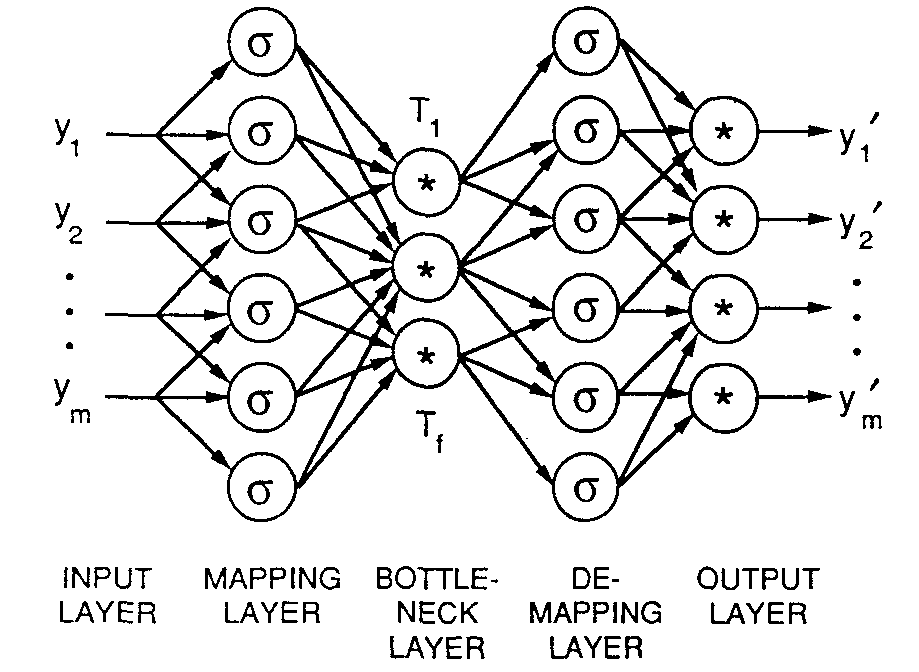
\includegraphics[width=0.6\linewidth]{\toplevelprefix/chapters/chapter5/figs/kramer1991nonlinearPCA.png}
  \caption{由 Kramer \cite{Kramer1991NonlinearPC} 提出的,使用深度为二的自联想神经网络进行非线性 PCA,用于编码和解码映射。}
  \label{fig:NLPCA}
\end{figure}

不幸的是,与上述 PCA 的情况不同,对于这些网络的参数 $\boldsymbol{\theta} = (\vW, \vb)$,通常没有闭式学习方案。因此,有人提出通过反向传播,以重构误差为监督信号来训练网络:
\begin{equation}\label{eq:nonlinear-pca-ch5}
  \min_{\boldsymbol{\theta}} \mathbb{E}[ \|\x - \x'(\boldsymbol{\theta})\|^2].
\end{equation}
与 PCA 的简单情况相比,我们使用相同的重构目标进行学习,但使用一个远为复杂的非线性模型类别来参数化和学习编码器和解码器。尽管像 Cybenko 的通用逼近性质表明,\textit{原则上}通过这个框架学习一致的自编码器是可能的——因为对于任何随机数据样本,只要有足够的参数,这样的自编码对就存在——但人们常常发现用梯度下降法找到它们是相当困难的。
此外,为了获得对高维真实世界数据(如图像)分布的足够信息量的重构目标和模型,所需的样本数量和隐藏节点数量可能非常巨大。
此外,作为衡量所学表示紧凑性的指标,瓶颈层 $\z$ 的(较低)维度通常是凭经验选择的。\footnote{在后来的工作 \cite{Hinton-1993} 中,Hinton 等人建议使用最小描述长度(MDL)原则来促进所学编码方案的紧凑性,其精神与本书中介绍的率失真度量非常相似。}
% \sdb{We can connect to Oja's here too: we learn with BP (don't just call GD)
% + it becomes nonlocal...}

\paragraph{通过更深的网络进行流形展平。}
根据深度网络的现代实践,这种经典的浅而宽的网络架构被认为很难通过反向传播(BP)进行有效和高效的训练,部分原因是 sigmoid 函数的梯度消失问题。因此,现代实践通常建议将非线性变换 $f$(或 $g$)进一步分解为更多层简单变换的复合,从而形成更深的网络架构 \cite{Hinton504},如图 \ref{fig:ccnet_layers} 所示。
在现代背景下,为了在复杂的真实世界数据分布(如图像)上取得良好性能,对基本重构成本 \eqref{eq:nonlinear-pca-ch5} 的进一步阐述也证明是必要的。

\begin{figure}[htb]
  \centering
  \begin{tikzpicture}
    \draw (-0.1, -0.2) .. controls (1, 0.25) .. (2.1, -0.1);
    \draw (2.1, -0.1) .. controls (1.75, 1) .. (2.1, 2);
    \draw (2.1, 2) .. controls (1, 1.75) .. (-0.1, 2);
    \draw (-0.1, 2) .. controls (0.25, 1) .. (-0.1, -0.2);

    \draw (0.35, 0.5) .. controls (0.7, 0.75) .. (0.85, 1.2);
    \draw (0.85, 1.2) .. controls (1.0, 1.4) .. (1.15, 1.2);
    \draw (1.15, 1.2) .. controls (1.3, 0.75) .. (1.65, 0.5);

    \node at (1, -0.5) {\(\x\)};

    \draw[->] (2.25, 1.25) -- (3.25, 1.25);
    \node at (2.75, 1.5) {\(\fl_{1}\)};

    \draw[->] (3.5, 1.25) -- (4.5, 1.25);
    \node at (4, 1.5) {\(\fl_{2}\)};

    \draw[->] (4.75, 1.25) -- (5.75, 1.25);
    \node at (5.25, 1.5) {\(\cdots\)};

    \draw[->] (6, 1.25) -- (7, 1.25);
    \node at (6.5, 1.5) {\(\fl_{L}\)};

    \draw[->] (7, 0.75) -- (6, 0.75);
    \node at (6.5, 0.5) {\(\re_{L}\)};

    \draw[->] (5.75, 0.75) -- (4.75, 0.75);
    \node at (5.25, 0.5) {\(\cdots\)};

    \draw[->] (4.5, 0.75) -- (3.5, 0.75);
    \node at (4, 0.5) {\(\re_{2}\)};

    \draw[->] (3.25, 0.75) -- (2.25, 0.75);
    \node at (2.75, 0.5) {\(\re_{1}\)};

    \draw (7.3, 0.1) -- (9.1, 0.1);
    \draw (9.1, 0.1) -- (9.1, 1.9);
    \draw (9.1, 1.9) -- (7.3, 1.9);
    \draw (7.3, 1.9) -- (7.3, 0.1);

    \node at (8.2, -0.5) {\(\z\)};

  \end{tikzpicture}
  \caption{展平与重构对 \((\fl, \re)\) 的构造过程示意图,其中编码器 \(\fl = \fl_{L} \circ \fl_{L - 1} \circ \cdots \circ \fl_{1}\) 由多个展平层复合而成,解码器 \(\re = \re_{1} \circ \re_{2} \circ \cdots \circ \re_{L}\) 由每个 \(\fl_{\ell}\) 的逆复合而成。}
  \label{fig:ccnet_layers}
\end{figure}

鉴于像 Cybenko 这样的通用逼近定理,人们最初可能会想知道,为什么在概念上,更深的自编码器会比浅层的更受青睐。
从纯粹的表达能力角度,我们可以通过一个与展平我们假设的数据分布所支撑的非线性流形任务相关的几何角度来理解这一现象。一种纯粹的构造性方法是逐步展平流形,这与我们在 \Cref{ch:compression,ch:representation} 中看到的扩散、去噪和压缩之间的相互作用是平行的。在几何设置中,与 $f_{\ell}$ 对应的增量\textit{展平过程}的形式是将流形上一点的邻域变换得更接近一个平坦的流形(即一个子空间),并强制与其余数据样本的局部一致性;解码器中相应的增量操作 $g_{\ell}$ 则撤销这一变换。这个过程精确地包含了关于底层流形的曲率信息,这些信息是从数据样本中估计出来的。只要有足够多的流形样本,并仔细实例化这个概念过程,就有可能将此过程实现为一个可验证地以白盒方式展平非线性流形的计算程序 \cite{Psenka-JMLR24}。然而,由于可扩展性不佳,该方法在应用于高维数据分布(如图像)时受到限制,这促使了更灵活的增量自编码方法的发展。

\subsection{稀疏自编码}
在上述自编码方案中,特征空间的维度 $d$ 通常被选择得远低于原始数据空间 $D$ 的维度,以便明确地强制或促进所学表示是低维的。然而,在实践中,我们通常不知道数据分布的内在维度。因此,自编码的特征空间维度的选择通常是凭经验进行的。在更一般的情况下,数据分布可以是一些低维子空间或子流形的混合。在这些情况下,强制所有特征共同处于一个单一的低维空间中已不再可行。

稀疏自编码器旨在解决其中一些限制。特别是,特征空间的维度可以等于甚至高于数据空间的维度,如图 \ref{fig:SAE} 所示。然而,特征被要求在特征空间中是高度稀疏的。因此,如果我们在目标 \eqref{eqn:autoencode-objective-ch5} 中除了编码率降低之外,还施加稀疏性作为简约性的度量,我们就会得到稀疏自编码的一个新目标:
\begin{equation}
  \min_{f, g}
  %\lambda
  \|\Z\|_0 - \Delta R(\Z) + d(\X, \hat \X),
  \label{eqn:autoencode-sparse}
\end{equation}
其中 $\ell^0$-“范数” $\|\spcdot\|_0$ 已知可以促进稀疏性。
这与我们在前一章 \ref{ch:representation} 中用来推导白盒 CRATE 架构的稀疏率降低目标 \eqref{eq:sparse-rr} 非常相似。

\begin{figure}
  \centering
  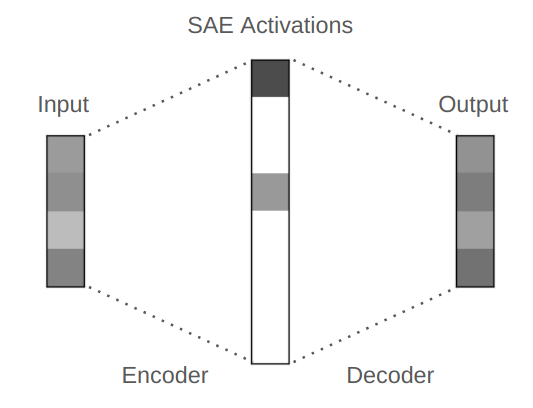
\includegraphics[width=0.5\linewidth]{\toplevelprefix/chapters/chapter5/figs/SAE_diagram.png}
  \caption{稀疏自编码器(SAE)的示意图,与图 \ref{fig:AE} 中的典型自编码器(AE)进行比较。}
  \label{fig:SAE}
\end{figure}

%\yima{There are other ways to promote the sparsity of the learned
% features $\Z$, including enforcing the frequency of activations for
%  each coordinate of $\z$ to be small... But here we can justify SAE
%  through its natural connection to sparse rate reduction. Anthropic
% AIseems to advocate that sparse autoencoding learns more
% interpretable features... }

作为一种端到端学习自编码对的方法,稀疏自编码在过去曾被实践过 \cite{Ranzato2006-oq},但几乎所有现代自编码框架都转而使用一种不同的、概率性的自编码框架,我们稍后将对此进行研究。
然而,值得注意的是,近年来,大量的注意力被投入到训练稀疏自编码器以\textit{解释预训练的大规模深度网络(如 Transformer)中的特征}上,其假设是这些网络中(先验地、不可解释的)特征是由可解释的底层特征的稀疏“叠加”组成的 \cite{elhage2022superposition}。
将这种方法与经典的稀疏自编码框架以及我们在本章中阐述的一般自编码方法进行对比是很有启发性的。
在稀疏自编码器训练和评估的最直接实例化中(参见 \citep{huben2024sparse, gao2025scaling}),从一个预训练的深度网络 $h$ 中收集大量来自不同输入 $\vx_i$ 的特征,而这些输入本身是根据期望的解释任务来选择的。\footnote{例如,输入 $\vx_i$ 可以对应于包含不同编程语言的计算机代码样本的文本,我们的任务是尝试在 Transformer 特征图 $h$ 中识别出与输入的不同显著方面相对应的可解释特征,例如特定的编程语言(在输入“类别”之间是不同的)或在当前位置插入匹配括号的需求(在输入“类别”之间是共同的)。我们在 \Cref{ch:applications} 中更详细地讨论了使用深度网络,特别是 Transformer,进行文本表示学习。}为简单起见,我们将使用 $h$ 来表示所讨论的预选特征图,其特征为 $D$ 维;给定 $N$ 个样本输入,令 $\vH \in \bR^{D \times N}$ 表示 $h$ 的完整特征矩阵。
然后,一个稀疏自编码器 $f : \bR^D \to \bR^d$ 及其解码器 $g : \bR^d \to \bR^D$ 通过 \Cref{eqn:autoencode-sparse} 中目标的松弛版本进行训练:
\begin{equation}\label{eq:sae-loss}
  \min_{f, g}
\lambda \|f(\vH)\|_1 + \frac{1}{2} \| \vH - g(f(\vH))) \|_2^2,
\end{equation}
其中稀疏自编码器 $f$ 通常采用单层神经网络的形式,即 $f(\vh_i) = \sigma(\vW_{\mathrm{enc}}(\vh_i - \vb) + \vb_{\mathrm{enc}})$,其中 $\sigma(x) = \max \{x, 0\}$ 是 ReLU 激活函数,而解码器 $g$ 是线性的,因此 $g(\vz_i) = \vW_{\mathrm{dec}}\vz + \vb$。
有趣的是,稀疏自编码器和解码器的这些简单架构可以看作与我们在 \Cref{ch:representation} 中阐述的展开优化方法所获得的架构完全类似,特别是与 CRATE 架构的 ISTA 模块(\Cref{eq:grad_lasso_ista})类似。
更准确地说,稀疏自编码器的编码器可以看作是在非负 LASSO 目标上进行的一步近端梯度下降,正如我们所见,这导致了 CRATE ISTA 模块;编码器和解码器的非对称结构可以类似地理解为 ISTA 模块中的前向映射(\Cref{eq:grad_lasso_ista})与稀疏化字典 $\vD$ 本身之间的差异,后者成为了解码器。
这种联系为改进稀疏自编码器的表示能力提出了一系列新的设计策略,但迄今为止似乎很少有被深入探索的。

\subsection{变分自编码}\label{sec:vae}

在 Hinton 和 Rumelhart \cite{Rumelhart1986} 之后的经典自编码概念中,尽管数据分布对于我们最终学习的表示至关重要,但它在公式化中扮演的角色却非常次要。实际上,在朴素的框架中,人们希望通过训练一个深度网络,用一个适当配置的瓶颈来表示 $\vz$,从而重构数据分布中的样本,使得学习到的编码器 $f$ 和 $g$ 自然而然地对应于数据的紧凑且结构化的特征表示。这在实践中很少发生。
一种至今仍在广泛应用的、经过改进的、更现代的自编码方法是\textit{变分自编码} \cite{Kingma2013-sb,Kingma2019-zh}。
我们将看到这个框架如何训练一个通过概率建模考虑推导出的变分自编码器(VAE),它既推广了经典的自编码器训练(通过最小化重构损失),又通过适当的正则化使其稳定。稍后,我们将看到如何更进一步,超越用于表示编码和解码映射 $f$ 和 $g$ 的深度网络的黑盒性质。

\subsubsection{自编码的概率视角}
在数据分布的流形模型中,关键的数学对象是数据分布的\textit{支撑集},即流形 $\cM$,以及数据在支撑集上的密度,比如 $p$。当我们从概率角度构建自编码时,我们通常将高维输入 $\vx$ 视为在 $\R^D$ 上具有支撑集和密度 $p$;可以认为,通过向支撑在流形 $\cM$ 上的(退化)分布添加少量噪声来获得这个密度 $p$,这与我们在第 \ref{ch:compression} 章中的去噪-扩散构造是一致的。
然后,生成式概率建模的目标是从样本 $\vx$ 中学习密度 $p$,比如从一类由 $\vtheta$ 参数化的模型 $p(\vx;\, \vtheta)$ 中学习。正如我们在第 \ref{ch:compression} 章中回顾的,实现这一目标的经典方法是通过最大似然估计:
\begin{equation*}\label{eq:VAE-MLE}
\max_{\vtheta}\, \bE_{\vx}[ \log p(\vx;\, \vtheta) ].
\end{equation*}
对于某些代表性的数据分布 $p$ %
% , including the
% manifold model without any further geometric constraints
% \cite{kiani2024hardness},
和足够表达力的模型类 $p(\vx;\, \vtheta)$,即使是比最大似然估计问题更简单的学习问题,在统计上也被认为是困难的 \cite{Yang1999-wb}。因此,利用 $\vx$ 具有低维结构的知识,通过寻求根据一个低维“潜”变量模型 $\vz$ 来分解分布 $p(\vx ;\, \vtheta)$ 是可取的。实际上,我们可以通过条件概率写出 $p(\vx, \vz ;\, \vtheta)
= p(\vz;\, \vtheta) p(\vx \mid \vz;\, \vtheta)$,以及
\begin{align*}
p(\vx; \vtheta) &= \int p(\vz;\, \vtheta) p(\vx \mid \vz;\, \vtheta) \odif \vz
\\
&=
\bE_{\vz \sim p(\,\cdot\,;\, \vtheta)}[ p(\vx \mid \vz;\, \vtheta) ].
\end{align*}
经典地,我们对数据分布 $p(\vx;\, \vtheta)$ 的模型对应于对潜分布 $p(\vz;\, \vtheta)$ 和条件分布 $p(\vx \mid \vz;\, \vtheta)$ 的选择。
即便如此,从这些潜分布计算数据分布的模型是难以处理的,除非在特殊情况下,这与我们在第 \ref{ch:classic} 章中研究的情况类似。
同样地,从数据中计算后验概率 $p(\vz \mid \vx;\, \vtheta)$,从而使我们能够将样本\textit{编码}到它们对应的潜变量,通常是难以处理的。
因此,在我们的生成模型的表达能力、其计算可处理性以及我们为了计算可处理性而对底层概率框架所做的任何近似的准确性之间存在一个权衡。
在驾驭这种权衡时,还需要一种灵活的计算方法来从数据中学习模型参数 $\vtheta$,这类似于最大似然目标。

在变分自编码框架中,我们通过三个关键的洞见来驾驭这种权衡:
\begin{enumerate}
\item 我们为 $\vz$ 和以 $\vz$ 为条件的 $\vx$ 假设\textit{简单}的分布,但使用深度网络使其参数以高度灵活的方式依赖于输入数据 $\vx$(在相关时)。
\item 我们将用于编码的后验概率 $p(\vz \mid \vx;\, \vtheta)$(其形式由我们对 $\vz$ 的建模选择通过贝叶斯法则隐含)替换为一个可处理的近似 $q(\vz \mid \vx;\, \veta)$,它有自己的参数 $\veta$。
\item 我们通过最大化似然函数 $p(\vx ;\, \vtheta)$ 的一个可处理的下界,即证据下界(ELBO),来联合学习 $\vtheta$ 和 $\veta$。
\end{enumerate}
我们将专注于 VAE 框架在实践中最有用的实例化,即先验 $p(\vz ;\, \vtheta)$ 和条件 $p(\vx \mid \vz;\,
\vtheta)$ 都是高斯分布的情况。也就是说,我们使用以下高斯分布:
\begin{align*}
\vz &\sim \cN(\Zero, \vI), \\
\vx \mid \vz &\sim \cN(g_1(\vz), \diag(e^{g_2(\vz)}) \vI),
\end{align*}
其中 $g = (g_1, g_2)$ 是带有参数 $\vtheta$ 的深度网络,对应于自编码器中的\textit{解码器}。
类似地,对于近似后验 $q(\vz \mid \vx;\, \veta)$,我们使用一个特殊的高斯分布,其参数由一个带有参数 $\veta$ 的编码器 MLP $f = (f_1, f_2)$ 给出:
\begin{equation*}
\vz \mid \vx \sim \cN(f_1(\vx), \diag(e^{f_2(\vx)}) \vI).
\end{equation*}
%\yima{We might need to elucidate what are the true implications of
% the above two assumptions on the forms of the two conditional
% distributions. How do these assumptions enforce certain desired
% structures of the representation and how are the structures related
% to what rate reduction and sparsity are promoting? }
这使得概率编码和解码变得简单:我们只需将数据 $\vx$ 映射到高斯分布的均值和方差参数以进行编码,反之亦然。
为了学习编码器和解码器,我们从最大似然目标 \Cref{eq:VAE-MLE} 出发,推导出一个方便的下界,称为证据下界,或 ELBO。从简单的代数操作开始
\begin{align*}
\log p(\vx;\, \vtheta) &=
\log \frac{p(\vx, \vz;\, \vtheta)}{p(\vz \mid \vx;\, \vtheta)}
\\
&=
\log \frac{p(\vx, \vz;\, \vtheta)}{q(\vz \mid \vx;\, \veta)}
+
\log \frac{q(\vz \mid \vx;\, \veta)}{p(\vz \mid \vx;\, \vtheta)},
\end{align*}
我们对 $\vz \sim q(\,\cdot\, \mid
\vx;\, \veta)$ 取期望,并使用吉布斯不等式(\Cref{thm:information-inequality})得到
\begin{equation*}
\log p(\vx;\, \vtheta)
\geq
\bE_{\vz \sim q(\,\cdot\, \mid \vx ;\, \veta)} \left[
  \log \frac{p(\vx, \vz;\, \vtheta)}{q(\vz \mid \vx;\, \veta)}
\right].
\end{equation*}
这个不等式的右边就是 ELBO;作为 $p(\vx;\, \vtheta)$ 的逐点对数似然的一个下界,其最大化在最大似然目标和计算可处理性之间提供了一个有原则的折衷。
有趣的是,上面的推导表明,其紧密性取决于近似后验 $q(\vz \mid \vx;\, \veta)$ 和真实后验 $p(\vz \mid \vx;\, \vtheta)$ 之间的 KL 散度,这意味着我们的近似后验越准确,最大化 ELBO 就越能导致最大化我们感兴趣的潜在目标,即数据的似然。因此,VAE 的目标是:
\begin{equation}\label{eq:elbo-objective}
\max_{\vtheta, \veta}\,
\bE_{\vx}
\bE_{\vz \sim q(\,\cdot\, \mid \vx ;\, \veta)} \left[
  \log \frac{p(\vx, \vz;\, \vtheta)}{q(\vz \mid \vx;\, \veta)}
\right].
\end{equation}
根据我们的推导,最大化这个目标对应于在最大化数据似然函数和最小化近似后验与真实后验之间的 KL 散度之间进行权衡,这在 VAE 的建模假设下是一个非常合理的目标。

\subsubsection{作为概率自编码的 VAE 训练}

存在一种通用方法,可以使用随机梯度下降和各种可处理的蒙特卡洛估计器来计算相关梯度,从而最大化 \Cref{eq:elbo-objective} 中的 ELBO 目标。然而,在我们上面做出的高斯假设下,这个任务更简单。在这种情况下,ELBO 读作
\begin{align*}
&\max_{\vtheta, \veta}\,
\bE_{\vx}
\bE_{\vz \sim q(\,\cdot\, \mid \vx ;\, \veta)} \left[
  \log \frac{p(\vx, \vz;\, \vtheta)}{q(\vz \mid \vx;\, \veta)}
\right]\\
=&
\max_{\vtheta, \veta}\,
\left\{
  \bE_{\vx}
  \bE_{\vz \sim q(\,\cdot\, \mid \vx ;\, \veta)} \left[
    \log p(\vx, \vz;\, \vtheta)
  \right]
  + \frac{d \log(2\pi e)}{2}
  % + \frac{1}{2}\sum_{i=1}^d f_{2, i}(\vx)
  + \frac{1}{2} \ip{ \bE_{\vx}[f_2(\vx)]}{\mathbf{1}}
\right\}
\\
\equiv &
\max_{\vtheta, \veta}\,
\left\{
  \bE_{\vx}
  \bE_{\vz \sim q(\,\cdot\, \mid \vx ;\, \veta)} \left[
    \log p(\vx \mid \vz;\, \vtheta)
    + \log p(\vz)
  \right]
  % +
  % \bE_{\vz \sim q(\,\cdot\, \mid \vx ; \veta)} \left[
  %   \log p(\vz)
  % \right]
  % + \frac{1}{2}\sum_{i=1}^d f_{2, i}(\vx)
  + \frac{1}{2} \ip{ \bE_{\vx}[f_2(\vx)]}{\mathbf{1}}
\right\}
\\
\equiv &
\max_{\vtheta, \veta}\,
\left\{
  2\bE_{\vx}\left[
    \bE_{\vz \sim q(\,\cdot\, \mid \vx ;\, \veta)} \left[
      \log p(\vx \mid \vz;\, \vtheta)
    \right]
    + \ip{ f_2(\vx) - e^{f_2(\vx)}}{\mathbf{1}}
    - \norm{f_1(\vx)}_2^2
    % + \frac{1}{2}\sum_{i=1}^d \left(
    %   f_{2, i}(\vx) - f_{1, i}^2(\vx) - e^{f_{2, i}(\vx)}
    % \right)
  \right]
\right\}, \labelthis \label{eq:elbo-for-gaussians}
\end{align*}
遵循在 \Cref{app:diffusion-denoising},\Cref{rem:gaussian-maxent} 中完成的高斯熵计算,其中 $\equiv$ 表示优化目标的等价性(在每种情况下,我们都移除了一些不改变优化问题解的加性常数)。
剩下的项对应于 ELBO 目标的“自编码”部分:直观上,它试图在潜变量 $\vz$ 根据近似后验(由编码器应用于数据样本 $\vx$ 生成)分布时,最大化由解码器生成的数据的似然,这是一种概率形式的自编码。
为了更直接地看到这一点,考虑一个特殊情况,即对于每个 $\vx$,近似后验都集中在其均值 $f_1(\vx)$ 上:这是其对数方差 $f_{2,i}(\vx) \to -\infty$ 对每个坐标 $i = 1, \dots, d$ 的极限情况。
为简单起见,再假设 $g_2(\vx) = \mathbf{1}$,使得解码器在每个坐标上都有恒定的单位方差。
那么,所讨论的损失项收敛到
\begin{align*}
\bE_{\vx}
\bE_{\vz \sim q(\,\cdot\, \mid \vx ;\, \veta)} \left[
  \log p(\vx \mid \vz;\, \vtheta)
\right]
&\to
\bE_{\vx} \left[
  \log p(\vx \mid f_1(\vx);\, \vtheta)
\right]
\\
% &=
% -\frac{1}{2} \bE_{\vx} \left[
%   (\vx - g_1\circ f_1(\vx))^\top \diag(e^{g_2\circ
% f_1(\vx)})^{-1} (\vx - g_1
%   \circ f_1(\vx))
%   % + \logdet\left( 2\pi \diag(e^{g_2 \circ f_1(\vx)}) \right)
%   + \sum_{i=1}^D (g_2 \circ f_1)_i(\vx)
% \right].
&\equiv
-\frac{1}{2} \bE_{\vx} \left[
  \|\vx - g_1\circ f_1(\vx)\|_2^2
\right].
\end{align*}
因此,对于一个高度自信的编码器(它确定性地将每个样本 $\vx$ 映射到 $\vz$-空间中的一个单点 $f_1(\vx)$)和一个各向同性的解码器,ELBO 最大化问题的“自编码”部分确实变成了一个经典的自编码目标!\footnote{在 $g_2$ 不固定为 $\mathbf{1}$ 的一般情况下,读者可以验证 ELBO 目标中的自编码项收敛到一个\textit{正则化}的经典自编码目标。}
同时,请注意,这个特殊情况实际上被 \Cref{eq:elbo-for-gaussians} 中的额外项排除了——这些项实际上对应于防止编码器坍缩的正则化项。
因此,一般的 ELBO 损失(\Cref{eq:elbo-objective,eq:elbo-for-gaussians})是经典自编码重构目标(\Cref{eq:nonlinear-pca-ch5})的一个严格推广,无论是在其数据保真度项方面,还是在包含正则化项方面。

\subsubsection{训练 VAE}
VAE 通常通过在 ELBO 目标(\Cref{eq:elbo-for-gaussians})上交替进行随机梯度上升来训练,给定来自真实数据分布的单个样本 $\vx$ 和来自 $\vz \sim q(\,\cdot\,\mid \vx;\, \veta)$ 的样本。特别是,标准做法是为每个样本 $\vx$ 收集并训练许多独立生成的样本 $\vz^{i}$。为了对 \Cref{eq:elbo-for-gaussians} 关于编码器参数 $\veta$ 求梯度,人们利用所谓的重参数化技巧,将 $\vz \sim q(\,\cdot\,\mid \vx;\, \veta)$ 写为
\begin{equation*}
\vz =_{\mathrm{d}} f_1(\vx) + \diag(e^{\tfrac{1}{2}f_2(\vx)}) \vg,
\quad \vg \sim
\cN(0, \vI),
\end{equation*}
其中 $=_{\mathrm{d}}$ 表示分布相等。然后,可以简单地为每个数据样本 $\vx$ 取许多独立的标准高斯样本 $\vg^{i}$,从近似后验生成相应的样本 $\vz^i$,并使用自动微分毫无问题地计算关于 $\veta$ 的梯度。


%The previous Chapter 6:

\section{学习自洽性表示}
\label{sec:self-consistency}

在前面的章节中,我们研究了通过(有损)压缩来学习低维分布的方法。正如我们在第 \ref{ch:intro} 章中提到并在前面章节中展示的,机器智能的进步在很大程度上依赖于找到计算上可行且高效的解决方案来实现所需的压缩,这些方案不仅在理论上是可计算或可处理的,而且在实践中也是可扩展的:
\begin{equation}
\mbox{\textbf{可计算}} \;
   \Longrightarrow \; \mbox{\textbf{可处理}} \; \Longrightarrow \; 
   \mbox{\textbf{可扩展}}。
\end{equation}
甚至可以说,过去十年左右机器智能取得的巨大进步,在很大程度上归功于可扩展模型和方法的发展,例如通过反向传播训练深度网络。拥有数十亿参数、在数万个强大 GPU 上用数万亿数据点训练的大型模型,在记忆现有知识方面展示了超人的能力。这使得许多人相信,随着模型规模的不断扩大,其“智能”将继续提高。

当我们为这些大型人造机器学习系统的工程奇迹喝彩时,我们也必须承认,与自然界的智能相比,这种提升机器智能的方法对资源的需求是不必要的。包括动物和人类在内的自然智能生物根本无法承受这种暴力学习方案,因为它们必须在能量、空间和时间预算非常有限的情况下运作,并受到许多严格的物理约束。

首先,有强有力的科学证据表明,我们的大脑不会进行全局的端到端反向传播来改进或纠正其预测。相反,神经科学界早就知道,我们的大脑通过局部闭环反馈来纠正错误,例如预测编码。这正是启发诺伯特·维纳在 20 世纪 40 年代发展反馈控制理论和控制论纲领的科学基础。

其次,我们在前面的章节中看到,为了学习一个一致的表示,需要学习一个双向的自编码:
\begin{equation}
 \X
\xrightarrow{\hspace{1mm} \mathcal{E} = f \hspace{1mm}} \Z  \xrightarrow{\hspace{1mm} \mathcal{D} = g \hspace{1mm}} \hat{\X}.
\end{equation}
它要求通过某种相似性度量 $d(\X, \hat \X)$ 来强制观测到的输入数据 $\X$ 和解码后的 $\hat \X$ 相互接近。在自然界中,动物或人类很少能直接接触到基准真相 $\X$。例如,我们永远无法直接获取场景中物体的真实 3D 形状、距离或动态。然而,我们都学会了非常准确和高效地估计和预测它们。因此,一个悬而未决的问题是,即使我们无法直接将我们的估计 $\hat \x$ 与基准真相 $\x$ 进行比较,我们如何能学习到 $\X$ 的真实分布。正如我们将在本章中看到的,答案也在于闭环反馈以及数据分布的低维性。



%This section introduces the concept of self-consistent for a system that learns autonomously.

% \begin{itemize}
%     \item Contrast: supervised representation learning needs human signal (class), self-supervised representation learning needs human signal (masking, augmentation), how to remove human signal from the mixture and get a autonomous system?
%     \item For full autonomy, need to work in both \(x\) space (actions, perceptions) and \(z\) space (representations, compression, planning?)
%     \item Measure distance in \(x\) space? Deficiencies in \(\ell^{2}\) loss, Wasserstein loss, etc 
%     \item Measure distance in \(z\) space? Only possible with compact and structured \(z\) space (say piecewise linear structure, i.e., mixture of subspaces)
%     \item Propose self-consistency: representation is consistent wrt itself --- features are consistent wrt their autoencoding 
% \end{itemize}


正如我们从前一章所知,为了确保一个表示是一致的,我们需要比较生成的 $\hat \X \sim p(\hat\x)$ 和原始的 $\X \sim p(\x)$,至少在分布上是这样。即使我们确实可以访问 $\X$ 和 $\hat \X$,从技术上讲,计算和最小化两个分布的距离也可能存在问题,特别是当分布的支撑集是低维的时候。在第 \ref{ch:compression} 章介绍的 KL 散度在两个没有重叠支撑集的分布之间甚至没有明确定义。

作为缓解上述计算和最小化两个(低维)分布之间距离困难的早期尝试,人们曾建议通过判别性方法来学习生成器/解码器 $g$ \cite{Tu-2007}。这一思路引出了{\em 生成对抗网络(GAN)}的思想 \cite{goodfellow2014generative}。它引入了一个判别器 $d$,通常由一个深度网络建模,以区分生成的样本 $\hat \X$ 和真实样本 $\X$:
\begin{equation}
 \Z \xrightarrow{\hspace{2mm} g(\z,\eta) \hspace{2mm}} \hat \X, \, \X \xrightarrow{\hspace{2mm} d(\x, \theta)\hspace{2mm}} \{\mathbf 0, \mathbf 1\}.
 \label{eqn:GAN}
\end{equation}
有人建议,我们可以尝试通过生成器 $g$ 和判别器 $d$ 之间的{\em 斯塔克伯格博弈}来对齐 $\hat \x$ 和 $\x$ 之间的分布:
\begin{equation}
\max_{\theta}\min_{\eta} \mathbb{E}_{p({\x})}\big[\log d(\x,\theta)\big] + \mathbb{E}_{p({\z})}\big[1 - \log d(\underbrace{g(\z,\eta)}_{\hat \x \,\sim\, p_g},\theta)\big].
\end{equation}
也就是说,判别器 $d$ 试图最小化真实样本 $\X$ 和生成样本 $\hat \X$ 之间的交叉熵,而生成器 $g$ 则试图做相反的事情。

可以证明,为上述斯塔克伯格博弈找到一个均衡点等价于最小化{\em Jensen-Shannon 散度}:
\begin{equation}
    \mathcal{D}_{JS}(p(\x), p_g(\hat \x)) = \mathcal{D}_{KL}\big(p \| (p + p_g)/{2}\big) + \mathcal{D}_{KL}\big(p_g \| (p + p_g)/{2}\big).
\end{equation}
请注意,与 KL 散度相比,即使两个分布的支撑集不重叠,JS 散度也是有明确定义的。然而,即使在两个高斯分布之间,JS 散度也没有闭式表达式,而 KL 散度有。此外,由于数据分布是低维的,JS 散度在优化时可能高度病态。\footnote{如 \cite{arjovsky2017wasserstein} 所示。}这或许可以解释为什么在许多后续的 GAN 变体中通常会使用许多额外的启发式方法。

因此,也有人建议用推土机(EM)距离或 Wasserstein 距离来代替 JS 散度。\footnote{粗略地说,对于具有潜在不重叠的低维支撑的分布,JS 散度的行为类似于 $\ell^0$-范数,而 EM 距离的行为类似于 $\ell^1$-范数。}然而,JS 散度和 W 距离都只能在两个一般分布之间进行近似计算。\footnote{例如,W 距离需要计算两个分布在所有 1-Lipschitz 函数上的期望的最大差值。}此外,无论是 JS 散度还是 W 距离,即使对于高斯分布,都没有闭式公式。\footnote{($\ell^1$-范数)W 距离可以被($\ell^2$-范数)W2 距离所界定,后者有闭式解 \cite{salmona2021gromovwasserstein}。然而,正如在高维几何中所熟知的,随着维度的增高,$\ell^1$-范数和 $\ell^2$ 范数在几何和统计性质上会显著偏离 \cite{Wright-Ma-2021}。这个界限可能会变得非常松。}

如果比较数据 $\X$ 和 $\hat \X$ 的分布很困难,那么是否有可能在编码器 $f$ 下比较学习到的特征 $\Z$ 与其像 $\hat \Z$:
\begin{equation}
 \X
\xrightarrow{\hspace{1mm} \mathcal{E} = f \hspace{1mm}} \Z  \xrightarrow{\hspace{1mm} \mathcal{D} = g \hspace{1mm}} \hat{\X} \xrightarrow{\hspace{1mm} \mathcal{E} = f \hspace{1mm}} \hat \Z?
\label{eqn:closed-autoencoding}
\end{equation}
这就引出了{\em 自洽性表示}的概念。
\begin{definition}[自洽性表示]\label{def:closed_loop}
    给定数据 \(\vX\),我们将一对函数 \((f \colon \cX \to \cZ, g \colon \cZ \to \cX)\) 称为一个\textit{自洽性表示},如果\textit{特征} \(\vZ = f(\vX)\) 是紧凑且结构化的,并且\textit{自编码特征} \(\hat{\vZ} \doteq f \circ g(\vZ)\) 与 \(\vZ\) \textit{接近}。
    \begin{enumerate}
        \item 如果 \(\vZ \approx \hat{\vZ}\) 在某种范数下以高概率成立,我们称其为\textit{样本级}自洽。
        \item 如果 \(\Law(\vZ) \approx \Law(\hat{\vZ})\),我们称该表示是\textit{分布级自洽}的。
    \end{enumerate}
\end{definition}


%\section{Closed-Loop Transcription}

\subsection{通过斯塔克伯格博弈进行闭环转录}\label{sec:closed-loop-transcription}
%This subsection introduces the closed-loop transcription framework and the game-theoretic formulation from \href{https://www.mdpi.com/1099-4300/24/4/456/htm}{the CTRL work}.

% \begin{itemize}
%     \item Closed loop transcription framework: feature quality for \(z\) and \(\hat{z}\) plus distance measure for \(z\) and \(\hat{z}\)
%     \item \(f\) plays role as encoder, discriminator, sensor; \(g\) plays role as decoder, generator, controller 
%     \item \(f\) maximizes above objective, \(g\) minimizes 
%     \item optimization strategy: gradient descent-ascent, or two-timescale GDA, or something else?
% \end{itemize}

% \begin{itemize}
%     \item also need to give an intro to game theory somewhere here...
% \end{itemize}

我们如何确保学到的表示是自洽的呢?像往常一样,我们假设 $\X = \cup_{j=1}^k \X_j$,其中每个样本子集 $\X_j$ 都属于一个低维子流形:$\X_j \subset \mathcal{M}_j, j = 1,\ldots, k$。遵循第 \ref{ch:general-distribution} 章中的记法,我们使用一个矩阵 $\bm \Pi^j(i,i) = 1$ 来表示样本 $i$ 属于类别 $j$ 的成员关系(否则 $\bm \Pi^j = 0$)。我们寻求一个连续映射 $f(\cdot,\theta): \x \mapsto \z$,将 $\X$ 映射到一个最优表示 $\Z = [\z^1, \ldots, \z^n] \subset \Re^{d \times n}$:
\begin{equation}
\bm X  \xrightarrow{\hspace{2mm} f(\x, \theta)\hspace{2mm}} \bm Z, 
\label{eqn:LDR}
\end{equation}
该映射最大化以下编码率降低(MCR$^2$)目标:
%\rc{vspace -2mm here if paper is too long}
\begin{equation}\label{eq:mcr2-formulation}
\begin{split}
\max_{\Z} \; \Delta R(\Z\, | \, \bm{\Pi}, \epsilon) %&= R(\Z, \epsilon) - R_c(\Z, \epsilon \mid  \bm{\Pi})\\
&\doteq \underbrace{\frac{1}{2}\log\det \Big(\I + {\alpha} \Z \Z^{*} \Big)}_{R(\Z\, | \epsilon)} \;-\; \underbrace{\sum_{j=1}^{k}\frac{\gamma_j}{2} \log\det\Big(\I + {\alpha_j} \Z \bm{\Pi}^{j} \Z^{*} \Big)}_{R_c(\Z \,|\bm \Pi, \epsilon)},
\end{split}
\end{equation}
其中 $\alpha=\frac{d}{n\epsilon^2}$,$\alpha_j=\frac{d}{\textsf{tr}(\bm{\Pi}^{j})\epsilon^2}$,$\gamma_j=\frac{\textsf{tr}(\bm{\Pi}^{j})}{n}$ 对于 $j = 1,\ldots, k$。

{通过最大化上述目标 \eqref{eq:mcr2-formulation} 来学习这样一个单向映射 \eqref{eqn:LDR} 的一个问题是,它倾向于扩展每个类别中特征的学习子空间的维度\footnote{如果特征空间 $d$ 的维度过高,最大化编码率降低可能会高估每个类别的维度。因此,为了学习一个好的表示,需要预先为特征空间选择一个合适的维度,正如在 \cite{yu2020learning} 的实验中所实现的。事实上,即使在最简单的单子空间情况下,即经典的 PCA \cite{Jolliffe1986},同样的“模型选择”问题也持续存在。据我们所知,在异构噪声情况下选择正确的主成分数量仍然是一个活跃的研究课题 \cite{hong2020selecting}。},正如我们在第 \ref{ch:compression} 章的第 \ref{sec:chap4-representation-learning-problem} 节中看到的。为了验证所学特征是否一致,即既没有高估也没有低估内在数据结构,我们可以考虑学习一个解码器 $g(\cdot,\eta): \z \mapsto  \x$,从表示 $\Z = f(\X,\theta)$ 回到数据空间 $\x$:$\hat \X = g(\Z, \eta)$:
\begin{equation}
    \X \xrightarrow{\hspace{2mm} f(\x, \theta)\hspace{2mm}} \Z \xrightarrow{\hspace{2mm} g(\z,\eta) \hspace{2mm}} \hat \X, 
    \label{eqn:autoencoding-ch6}
\end{equation}
并检查 $\X$ 和 $\hat \X$ 的接近程度。这就构成了一个自编码,这正是我们在前一章 \ref{ch:autoencoding} 中广泛研究的内容。

\paragraph{在特征空间中测量距离。}
然而,正如我们上面讨论的,如果我们没有选择计算 $\X$ 和 $\hat \X$ 之间的距离,我们只能选择比较它们对应的特征 $\Z$ 和 $\hat \Z = f(\hat \X, \theta)$。请注意,在 MCR$^2$ 目标下,得到的 $\Z$ 或 $\hat \Z$ 的分布倾向于是分段线性的,因此它们的距离可以更容易地计算。更准确地说,由于每个类别的特征 $\Z_j$ 和 $\hat{\Z}_j$ 都接近于一个低维子空间/高斯分布,它们的“距离”可以通过编码率降低来衡量,{其中 \eqref{eq:mcr2-formulation} 被限制在两个大小相等的集合上}:
\begin{equation}
\Delta R\big(\Z_j, \hat{\Z}_j\big) \doteq R\big(\Z_j \cup \hat{\Z}_j\big) - \frac{1}{2} \big( R\big(\Z_j) + R\big(\hat \Z_j)\big).
\end{equation}
$\Z$ 和 $\hat \Z$ 之间的总距离由下式给出:
\begin{equation}
d(\Z, \hat \Z) \doteq   \sum_{j=1}^k \Delta R\big(\Z_j, \hat{\Z}_j\big) =  \sum_{j=1}^k \Delta R\big(\Z_j, f(g(\Z_j, \eta),\theta)\big).
\label{eqn:Z-distance}
\end{equation}


如果我们有兴趣辨别原始数据 $\X$ 和其解码后的 $\hat \X$ 分布中的{\em 任何}差异,我们可以将特征编码器 $f(\cdot, \theta)$ 视为一个“判别器”,通过简单地最大化距离 $d(\X, \hat \X)$ 来{\em 放大}所有 $\X_j$ 和 $\hat \X_j$ 对之间的任何差异:
\begin{equation}
\max_f d(\Z, \hat \Z) = \max_{\theta} \sum_{j=1}^k \Delta R\big(\Z_j, \hat{\Z}_j\big) = \max_{\theta} \sum_{j=1}^k \Delta R\big(f(\X_j,\theta), f(\hat{\X}_j,\theta)\big).
    \label{eqn:max-distance}
\end{equation}
也就是说,$\X$ 和 $\hat \X$ 之间的“距离”可以被衡量为这两组中所有类别对之间可实现的最大编码率降低。在某种程度上,这衡量了解码后的 $\hat \X$ 与原始数据 $\X$ 的对齐程度——从而衡量编码器 $f$ 的“单射性”的好坏。请注意,这种判别性度量与 GAN \eqref{eqn:GAN} 的思想是一致的,后者试图将 $\X$ 和 $\hat \X$ 分成两类,用交叉熵来衡量。

然而,这里的判别性编码器 $f$ 自然地推广到数据分布是多类别和多模态的情况,并且判别性是用一个更精细的度量——编码率降低——来衡量的,而不是 GAN 中典型的二分类损失(例如交叉熵)。也就是说,我们可以将编码器 $f$ 视为一个广义的判别器,它取代了 \eqref{eqn:GAN} 中的二元分类器 $d$:
\begin{equation}
 \Z \xrightarrow{\hspace{2mm} g(\z,\eta) \hspace{2mm}} \hat \X, \, \X \xrightarrow{\hspace{2mm} f(\x, \theta)\hspace{2mm}} \{\hat \Z, \Z\}.
 \label{eqn:closed-loop-GAN}
\end{equation}
整个流程可以用下面的“闭环”图来说明:}
\begin{equation}
    \X \xrightarrow{\hspace{2mm} f(\x, \theta)\hspace{2mm}} \Z \xrightarrow{\hspace{2mm} g(\z,\eta) \hspace{2mm}} \hat \X \xrightarrow{\hspace{2mm} f(\x, \theta)\hspace{2mm}} \ \hat \Z, 
\end{equation}
其中整个模型的参数为:$\Theta = \{\theta, \eta\}$。图 \ref{fig:auto-encoding-closed} 显示了整个过程。

\begin{figure}[t]
{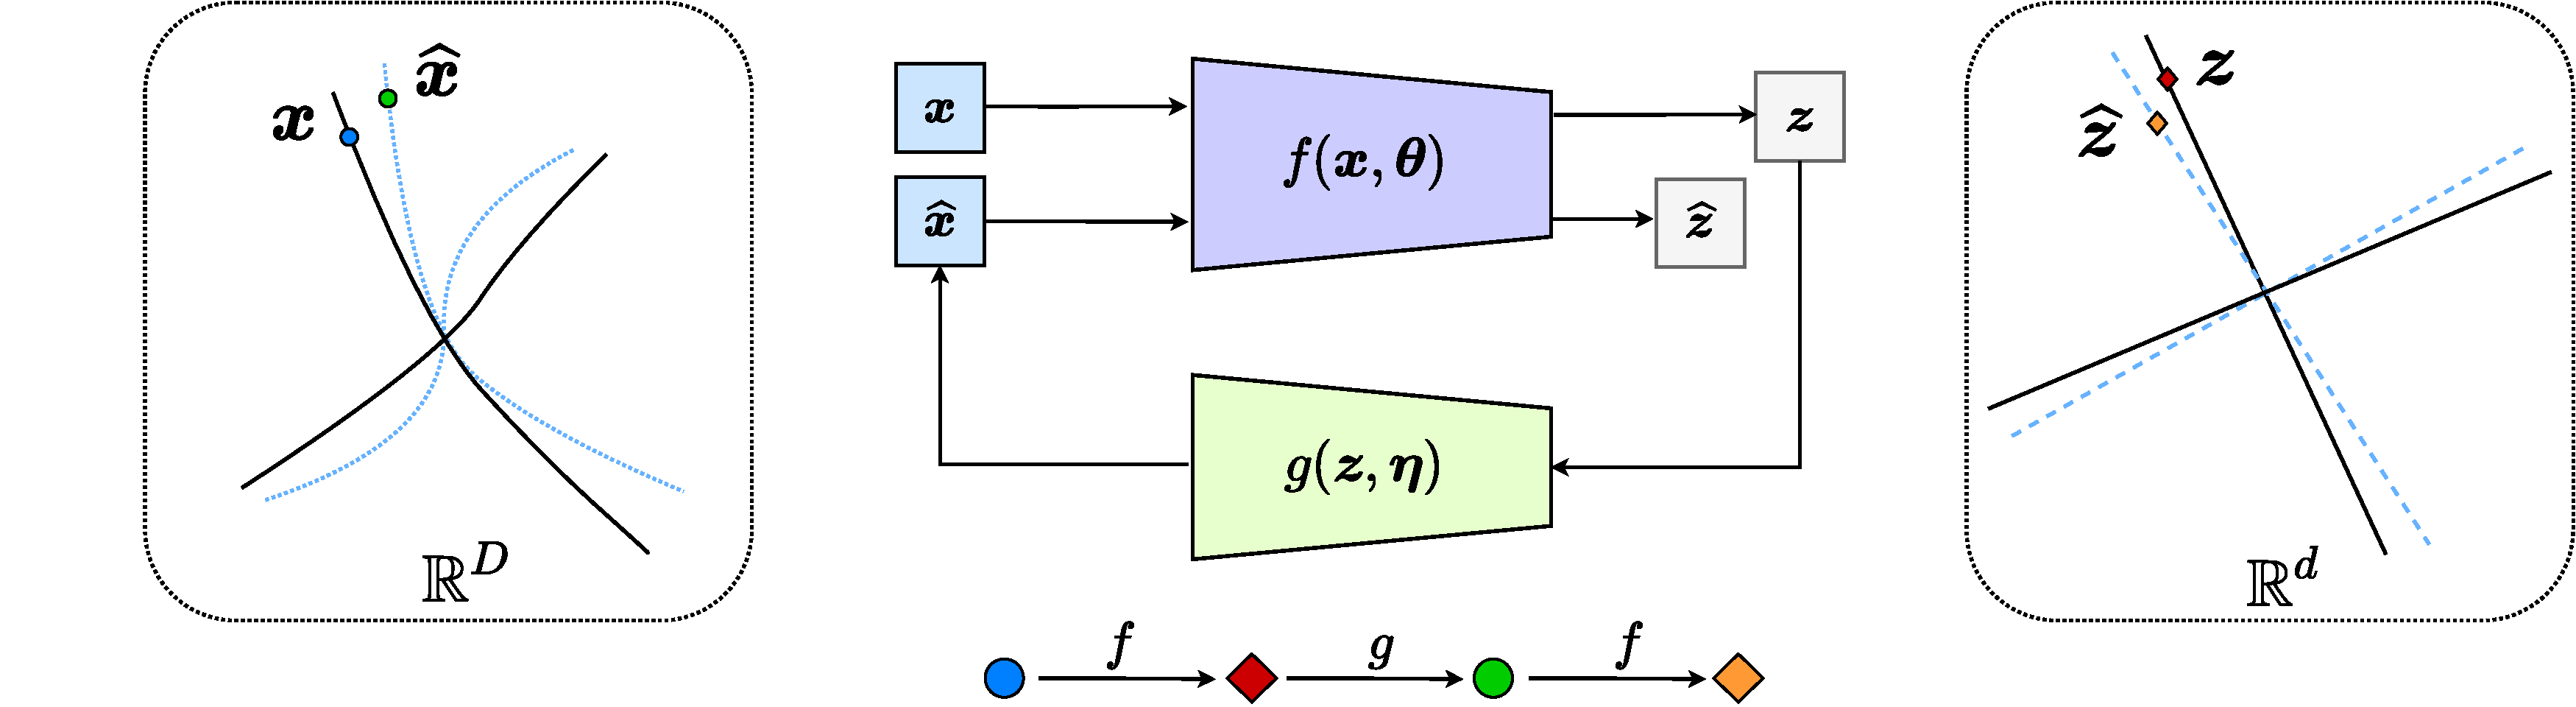
\includegraphics[width=1.0\linewidth]{\toplevelprefix/chapters/chapter5/figs/diagrams_redu_gan_2.pdf}}
\caption{{\bf 闭环转录。} 编码器 $f$ 具有双重角色:它通过最大化 $\z$ 的编码率降低来学习数据 $\x$ 的表示 $\z$,同时它也是数据 $\x$ 和解码后的 $\hat \x$ 之间任何差异的“反馈传感器”。解码器 $g$ 也具有双重角色:它是一个“控制器”,用于纠正 $\x$ 和 $\hat \x$ 之间的差异,同时它也旨在最小化所学表示的整体编码率。} \label{fig:auto-encoding-closed} 
\end{figure}


\paragraph{编码器和解码器作为双人博弈。}
显然,为了确保所学的自编码是自洽的,解码器 $g(\cdot, \eta)$ 的主要目标是{\em 最小化} $\Z$ 和 $\hat \Z$ 之间的距离。也就是说,为了学习 $g$,我们希望最小化距离 $d(\Z, \hat \Z)$:
\begin{equation}
\min_g d(\Z, \hat \Z) \doteq \min_\eta  \sum_{j=1}^k \Delta R\big(\Z_j, \hat{\Z}_j\big) =  \min_\eta  \sum_{j=1}^k \Delta R\big(\Z_j, f(g(\Z_j, \eta),\theta)\big),
\label{eqn:min-distance}
\end{equation}
其中 $\Z_j = f(\X_j,\theta)$ 且 $\hat \Z_j = f(\hat{\X}_j,\theta)$。

\begin{example}
有人可能会问,为什么我们需要映射 $f(\cdot, \theta)$ 通过最大化 $\max_\theta \Delta R\big(f(\X,\theta), f(\hat \X,\theta)\big)$ 来充当 $\X$ 和 $\hat \X$ 之间的判别器。图 \ref{fig:decoder} 给出了一个简单的说明:可能存在许多解码器 $g$ 使得 $f\circ g$ 是一个恒等(Id)映射。对于特征空间中子空间 $S_{\z}$ 内的所有 $\z$,都有 $f\circ g(\z) = \z$。然而,$g\circ f$ 不一定是原始分布 $S_{\x}$(这里为简单起见画成一个子空间)中 $\x$ 的自编码映射。也就是说,$g\circ f(S_{\x}) \not\subset S_{\x}$,更不用说 $g\circ f(S_{\x}) = S_{\x}$ 或 $g\circ f(\x) = \x$ 了。可以预见,如果不仔细控制 $g$ 的像,这种情况很可能会发生,特别是当 $\x$ 的分布支撑在原始高维数据空间中是极低维的时候。
\end{example}
\begin{figure}
%\vspace{-1mm}
\centering{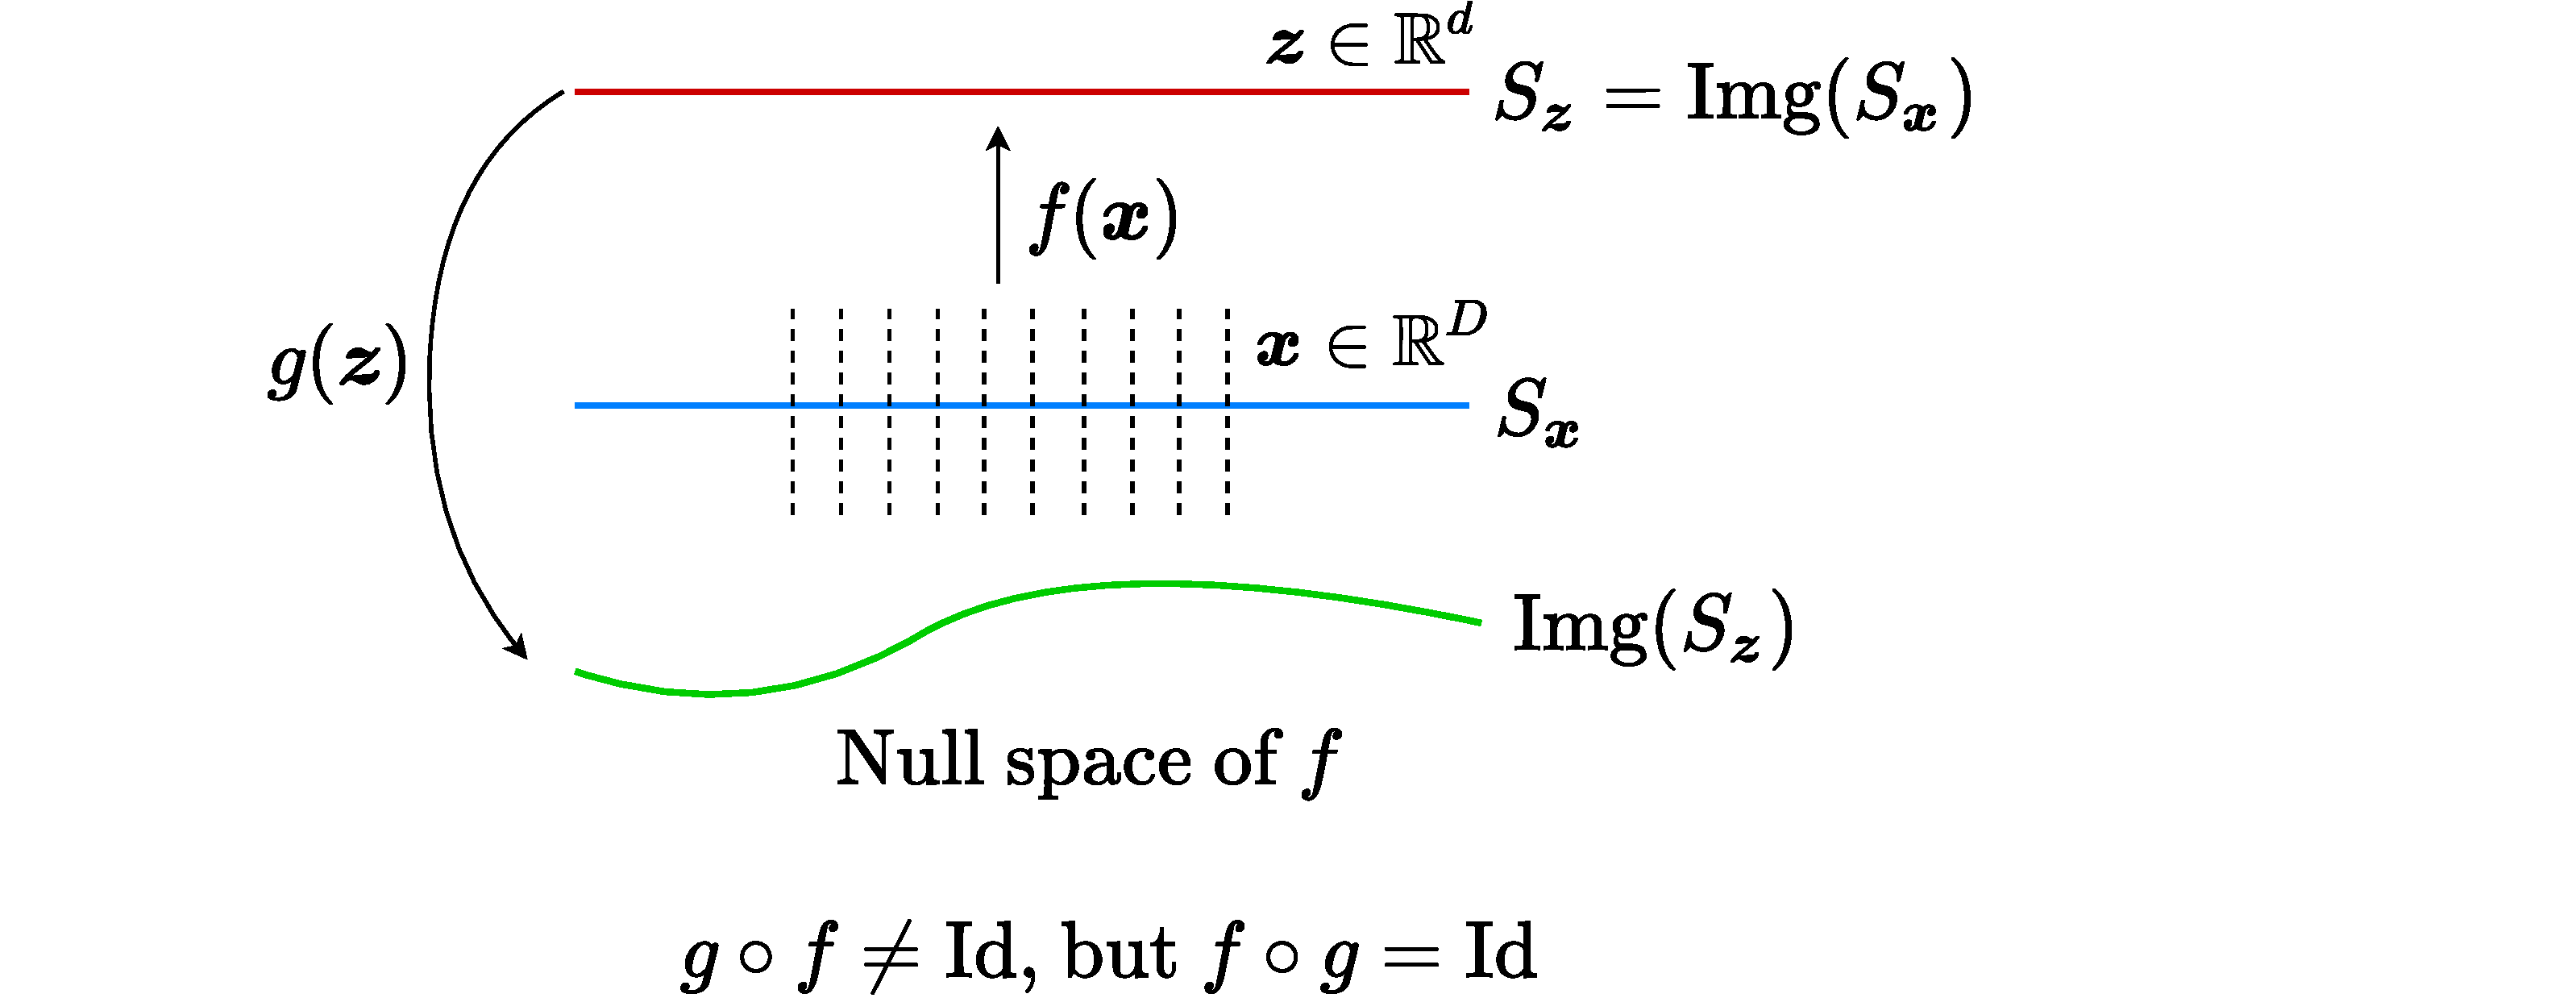
\includegraphics[width=3.0in]{\toplevelprefix/chapters/chapter5/figs/diagrams_fig1.pdf}}
\caption{\textbf{高维空间中低维子流形的嵌入。} $S_{\x}$(蓝色)是原始数据 $\x$ 的子流形;$S_{\z}$(红色)是 $S_{\x}$ 在映射 $f$ 下的像,代表学习到的特征 $\z$;绿色曲线是特征 $\z$ 在解码映射 $g$ 下的像。} \label{fig:decoder}
\end{figure} 

比较 \eqref{eqn:min-distance} 和 \eqref{eqn:max-distance} 在相同距离度量上的收缩和对比性质,我们看到编码器 $f(\cdot, \theta)$ 和解码器 $g(\cdot, \eta)$ 的角色自然地表现为“{\bf 一个双人博弈}”:{\em 当编码器 $f$ 试图放大原始数据与其转录数据之间的差异时,解码器 $g$ 则旨在最小化这种差异。} 现在为方便起见,我们定义“闭环编码”函数:
\begin{equation}
    h(\x, \theta, \eta) \doteq f\big(g\big(f(\x, \theta), \eta\big), \theta\big): \; \x \mapsto \hat \z.
\end{equation}

理想情况下,我们希望这个函数非常接近 $f(\x, \theta)$,或者至少它们像的分布应该接近。有了这个记法,结合 \eqref{eqn:min-distance} 和 \eqref{eqn:max-distance},$\X$ 和 $\hat \X$ 之间的一个闭环“距离”概念可以计算为以下斯塔克伯格博弈(参见 \Cref{sec:minimax})的{\em 均衡点},该博弈在编码率降低方面具有相同的效用:
\begin{equation}
\mathcal{D}(\X, \hat \X) \doteq  \max_\theta \min_\eta \sum_{j=1}^k \Delta R\big(f(\X_j,\theta), h(\X_j,\theta,\eta)\big).
    \label{eq:MCR2-GAN-pair}
\end{equation}

请注意,这只衡量了原始数据(的特征)与其转录版本之间的差异。它没有衡量表示 $\Z$(或 $\hat \Z$)对于 $\X$(或 $\hat \X$)内多个类别的优劣程度。为此,我们可以将上述距离与原始的 MCR$^2$ 型目标 \eqref{eq:mcr2-formulation} 结合起来:即为 $\X$ 学习到的 LDR $\Z$ 的编码率降低 $\Delta R(\Z)$ 和为解码后的 $\hat \X$ 学习到的 $\hat \Z$ 的编码率降低 $\Delta R(\hat \Z)$。请注意,虽然编码器 $f$ 试图{\em 最大化}数据 $\X$ 的特征 $\Z$ 的多类别编码率降低,但解码器 $g$ 应该{\em 最小化}解码后的 $\hat \X$ 的多类别特征 $\hat \Z$ 的编码率降低。也就是说,解码器 $g$ 试图使用最小的编码率来实现良好的解码质量。

因此,用于学习闭环转录的整体“多类别”斯塔克伯格博弈,命名为 CTRL-Multi,是
\begin{eqnarray}
&&\max_\theta \min_\eta \mathcal{T}_{\X}(\theta, \eta) \\
&\doteq& \underbrace{\Delta R\big(f(\X,\theta)\big)}_{\text{扩张性编码}} + \underbrace{\Delta R\big(h(\X,\theta, \eta)\big)}_{\text{压缩性解码}} + \sum_{j=1}^k \underbrace{\Delta R\big(f(\X_j,\theta), h(\X_j,\theta,\eta)\big)}_{\text{对比性编码与收缩性解码}} \nonumber \\
&=& \Delta R\big(\Z(\theta) \big) + \Delta R\big(\hat \Z(\theta, \eta)\big) + \sum_{j=1}^k \Delta R\big(\Z_j(\theta), \hat \Z_j(\theta, \eta) \big),
    \label{eq:MCR2-GAN-objective}
\end{eqnarray}
受限于对第一项和第二项的某些约束(上界或下界)。

% \begin{adjustwidth}{-\extralength}{0cm}
% \centering %% If there is a figure in wide page, please release command \centering

% \end{adjustwidth}

请注意,如果没有与生成部分 $h$ 相关联的项,或者所有这些项都固定为常数,则上述目标正是第 \ref{ch:compression} 章中介绍的原始 MCR$^2$ 目标。在无监督设置中,如果我们将每个样本(及其增强)视为其自己的类别,则上述公式完全保持不变。类别数 $k$ 就是独立样本的数量。此外,请注意,上述博弈的目标函数仅依赖于数据 $\X$(的特征),因此可以学习编码器和解码器(参数)而无需采样或匹配任何额外的分布(这在 GAN 或 VAE 中通常是必需的)。

作为一个特例,如果 $\X$ 只有一个类别,斯塔克伯格博弈就简化为一种特殊的“二分类”或“二元”形式,\footnote{因为前两个编码率降低项自动变为零} 命名为 CTRL-Binary,
\begin{equation}
 \max_\theta \min_\eta \mathcal{T}^b_{\X}(\theta, \eta) \doteq \Delta R\big(f(\X,\theta), h(\X,\theta,\eta)\big) = \Delta R\big(\Z(\theta), \hat \Z(\theta, \eta)\big), 
    \label{eq:MCR2-GAN-objective-binary}
\end{equation}
在 $\X$ 和解码后的 $\hat\X$ 之间,将 $\X$ 和 $\hat \X$ 视为两个类别 $\{\bm 0, \bm 1\}$。请注意,这种二元情况类似于原始 GAN \eqref{eqn:GAN} 的公式。我们的公式采用了一种更精细的编码率降低度量,而不是使用交叉熵,这在第 \ref{ch:compression} 章中已被证明可以促进所学表示的多样性。

有时,即使 $\X$ 包含多个类别/模态,人们仍然可以将所有类别一起视为一个类别。然后,上述二元目标就是将所有类别的联合分布与其解码后的 $\hat \X$ 对齐。这通常比多类别任务 \eqref{eq:MCR2-GAN-objective} 更容易实现,因为它不需要为数据学习更精细的多类别 CTRL,我们稍后将在实验中看到。请注意,上述公式的一个良好特性是,{\em 目标中的所有量都是根据所学特征的编码率降低来衡量的}(假设特征最终变为子空间高斯分布)。

有人可能会注意到,上述学习框架的灵感来自于反馈控制系统中广泛实践的闭环误差校正。闭环机制用于在两个编码和解码网络之间形成一个整体的反馈系统,以校正数据 $\x$ 和解码后的 $\hat \x$ 之间分布的任何“误差”。用控制理论的术语来说,可以将编码网络 $f$ 视为误差反馈的“传感器”,而将解码网络 $g$ 视为误差校正的“控制器”。然而,请注意,这里的控制“目标”不是一个标量,也不是一个有限维向量,而是一个连续分布——为了使 $\hat \x$ 的分布与数据 $\x$ 的分布相匹配。这通常是一个无限维空间中的控制问题。$f$ 试图建模的子流形的可能微分同胚空间是无限维的 \cite{Lee2002IntroductionTS}。理想情况下,我们希望当传感器 $f$ 和控制器 $g$ 最优时,$\x$ 的分布成为闭环的“不动点”,而 $\z$ 的分布达到一个紧凑的线性判别表示。因此,极小极大程序 \eqref{eq:MCR2-GAN-objective} 和 \eqref{eq:MCR2-GAN-objective-binary} 也可以解释为误差反馈传感器和误差减少控制器之间的博弈。

剩下的问题是,上述框架是否真的能学习给定数据集的良好(自编码)表示?在我们给出一些正式的理论论证(在下一小节)之前,我们先展示一些经验结果。

\paragraph{可视化特征 $\Z$ 和解码特征 $\hat \Z$ 的相关性。} 我们可视化了从多类别目标 \eqref{eq:MCR2-GAN-objective} 在 MNIST、CIFAR-10 和 ImageNet(10 类)上学习到的 $\Z$ 和 $\hat{\Z}$ 之间的余弦相似度,这表明 $\hat{\z} = f\circ g(\z)$ 与 $\z$ 的接近程度。图 \ref{fig:justifyz=z} 中的结果显示,$\Z$ 和 $\hat{\Z}$ 在每个类别内都对齐得很好。MNIST 的块对角模式比 CIFAR-10 和 ImageNet 的更清晰,因为 CIFAR-10 和 ImageNet 中的图像具有更多样化的视觉外观。

\begin{figure}[t]
    \begin{subfigure}[t]{0.3\textwidth}
        \centering
        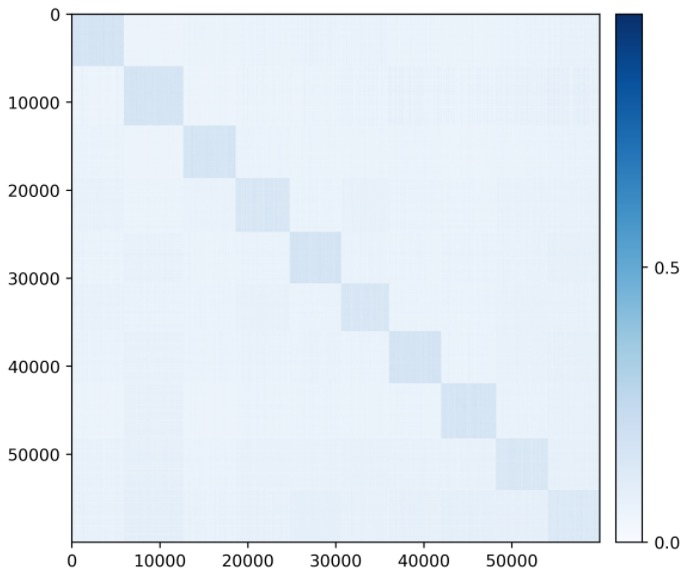
\includegraphics[width=\textwidth]{\toplevelprefix/chapters/chapter5/figs/MNIST_MNIST_ZZhat_heatmap_epo200.png}
        \caption{MNIST}
    \end{subfigure}
    \hfill
    \begin{subfigure}[t]{0.3\textwidth}
        \centering
        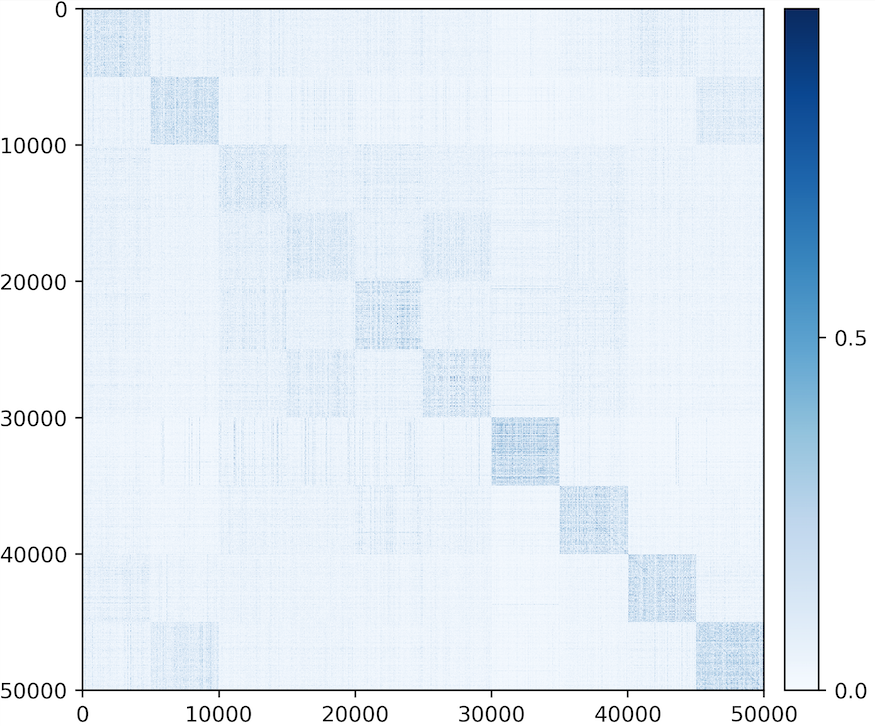
\includegraphics[width=\textwidth]{\toplevelprefix/chapters/chapter5/figs/cifar_heatmat_cifar.png}
        \caption{CIFAR-10}
    \end{subfigure}
    \hfill
    \begin{subfigure}[t]{0.3\textwidth}
        \centering
        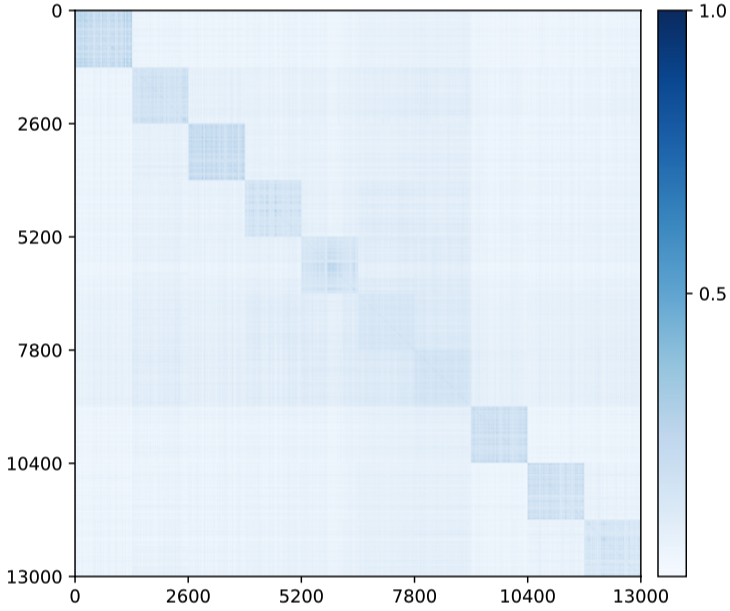
\includegraphics[width=\textwidth]{\toplevelprefix/chapters/chapter5/figs/Imagenet_heatmat_epoch200000.png}
        \caption{ImageNet}
    \end{subfigure}
    \caption{可视化 $\Z$ 和 $\hat{\Z}$ 之间的对齐:特征空间中(a)MNIST、(b)CIFAR-10 和(c)ImageNet-10-Class 的 $|\Z^\top \hat{\Z}|$。}
    \label{fig:justifyz=z}
\end{figure}
 


%$\Z$ and $\hat{\Z}$ are the inter-media and output results from CTRL. Both experiments are training and visualizing on train set with Equation~(\ref{eq:MCR2-GAN-objective}). The results show that $\Z$ and $\hat{\Z}$ are aligned well. For the result on MNIST, the diagonal of the matrix is clear compare with the rest part which means the feature space $\Z$ and $\hat{\Z}$ of MNIST can be aligned well by CTRL. CIFAR-10 is a little bit worse than MNIST, but still clear. Even for ImageNet, the diagonal of the matrix is still acceptable. With the more and more complexity of the data, it is reasonable for the decrease of the CTRL alignment ability.



\paragraph{可视化数据 $\X$ 和解码后的 $\hat \X$ 的自编码。} 我们比较了 MNIST、CIFAR-10 和 ImageNet(10 类)上的一些代表性 $\X$ 和 $\hat{\X}$,以验证 $\hat \x = g\circ f(\x)$ 与 $\x$ 的接近程度。结果如图 \ref{fig:justifyx=x} 所示,可视化是从训练样本创建的。从视觉上看,自编码的 $\hat \x$ 忠实地捕捉了其各自训练样本 $\x$ 的主要视觉特征,特别是姿态、形状和布局。对于像 MNIST 这样更简单的数据集,自编码图像几乎与原始图像相同。

%Both experiments are training and visualizing on train set with Equation~(\ref{eq:MCR2-GAN-objective}). The results show that $\X$ and $\hat{\X}$ are aligned which means CTRL has the property to enforce the auto-encoding. One amazing thing is that the CTRL can make exactly one-one mapping on MNIST (compare Figure~\ref{fig:justifyx=x}(a) and Figure~\ref{fig:justifyx=x}(b)).

\begin{figure}[t]
    \begin{subfigure}[t]{0.3\textwidth}
        \centering
        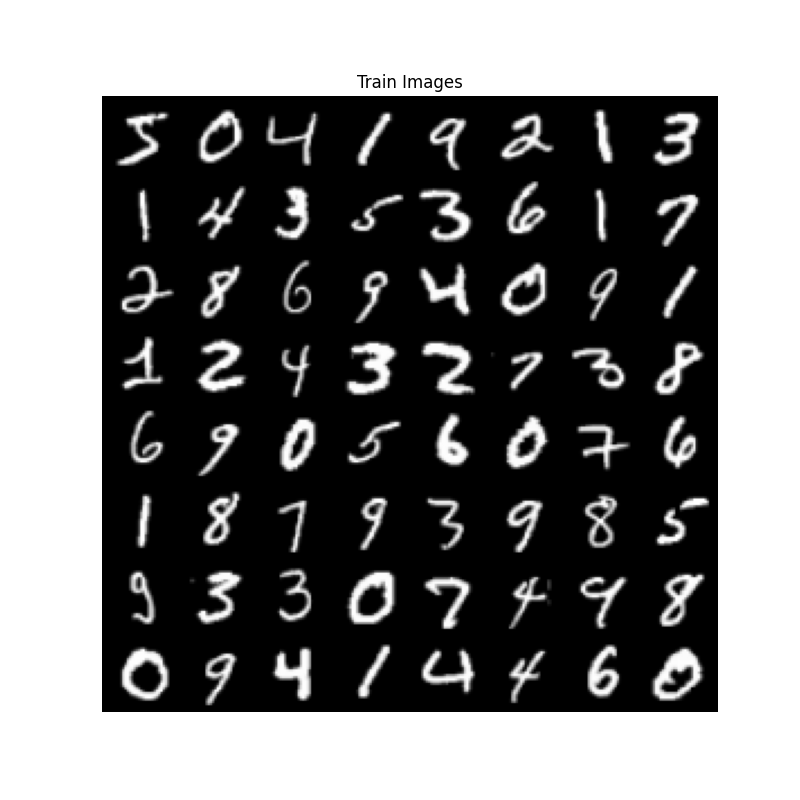
\includegraphics[width=\textwidth]{\toplevelprefix/chapters/chapter5/figs/MNIST_MNIST_train_images_epoch200.png}
        \caption{{\small MNIST $\X$}}
    \end{subfigure}
    \hfill
    \begin{subfigure}[t]{0.3\textwidth}
        \centering
        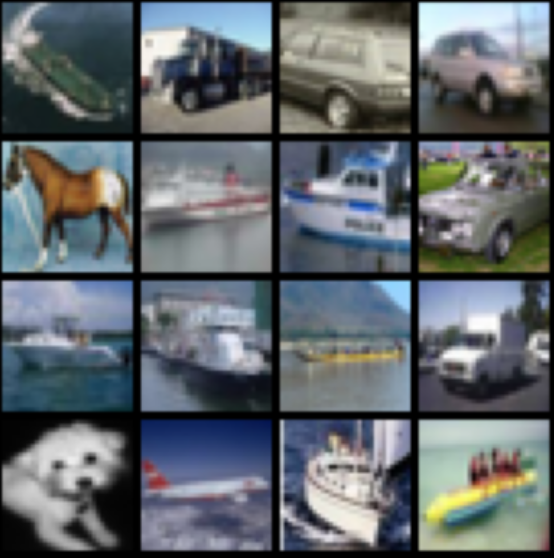
\includegraphics[width=\textwidth]{\toplevelprefix/chapters/chapter5/figs/cifar_input.png}
        \caption{{\small CIFAR-10 $\X$}}
    \end{subfigure}
    \hfill
    \begin{subfigure}[t]{0.3\textwidth}
        \centering
        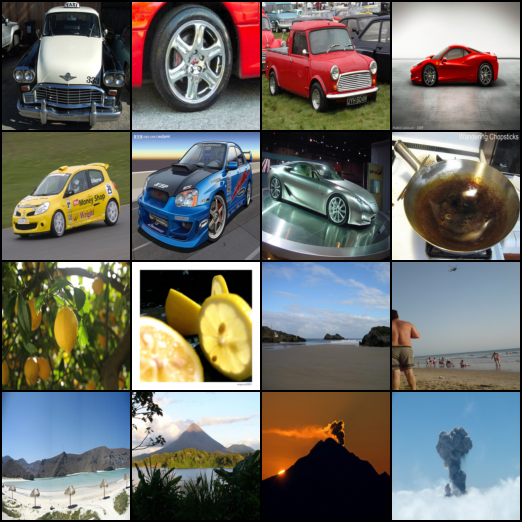
\includegraphics[width=\textwidth]{\toplevelprefix/chapters/chapter5/figs/Imagenet_input.png}
        \caption{{\small ImageNet $\X$}}
    \end{subfigure}

    \begin{subfigure}[t]{0.3\textwidth}
        \centering
        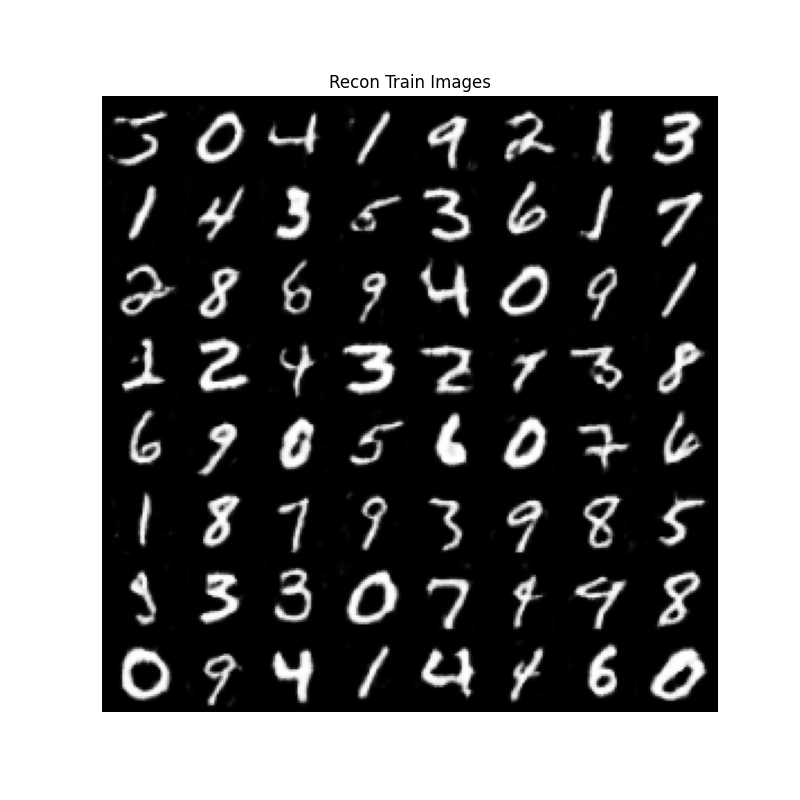
\includegraphics[width=\textwidth]{\toplevelprefix/chapters/chapter5/figs/MNIST_MNIST_train_recon_images_epoch200_multi.png}
        \caption{{\small MNIST $\hat{\X}$}}
    \end{subfigure}
    \hfill
    \begin{subfigure}[t]{0.3\textwidth}
        \centering
        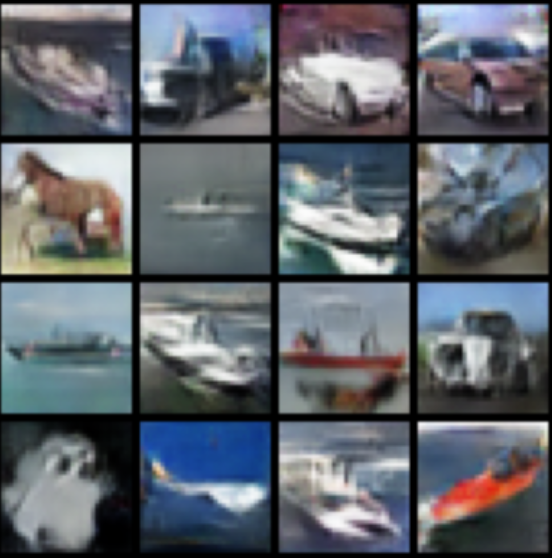
\includegraphics[width=\textwidth]{\toplevelprefix/chapters/chapter5/figs/cifar_reconstruct.png}
        \caption{{\small CIFAR-10 $\hat{\X}$}}
    \end{subfigure}
    \hfill
    \begin{subfigure}[t]{0.3\textwidth}
        \centering
        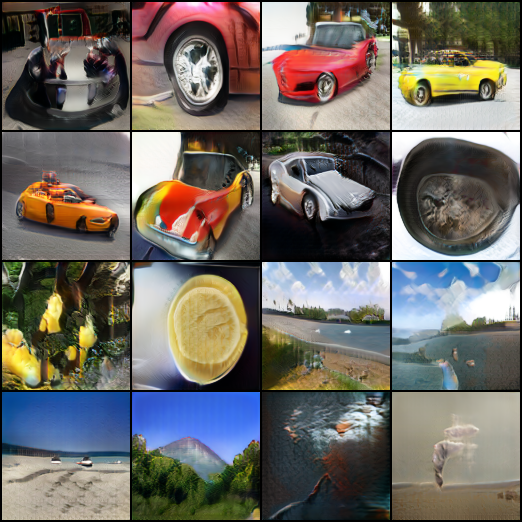
\includegraphics[width=\textwidth]{\toplevelprefix/chapters/chapter5/figs/Imagenet_reconstruct.png}
        \caption{{\small ImageNet $\hat{\X}$}}
    \end{subfigure}
    \caption{可视化学习到的闭环转录的自编码属性($\x \approx \hat{\x} = g\circ f(\x)$)在 MNIST、CIFAR-10 和 ImageNet 上的表现(放大以获得更好的可视化效果)。}
    \label{fig:justifyx=x}
\end{figure}
% \begin{figure}
%      \footnotesize
%      %\centering
%      \subfigure[{\small MNIST $\X$}]{
%          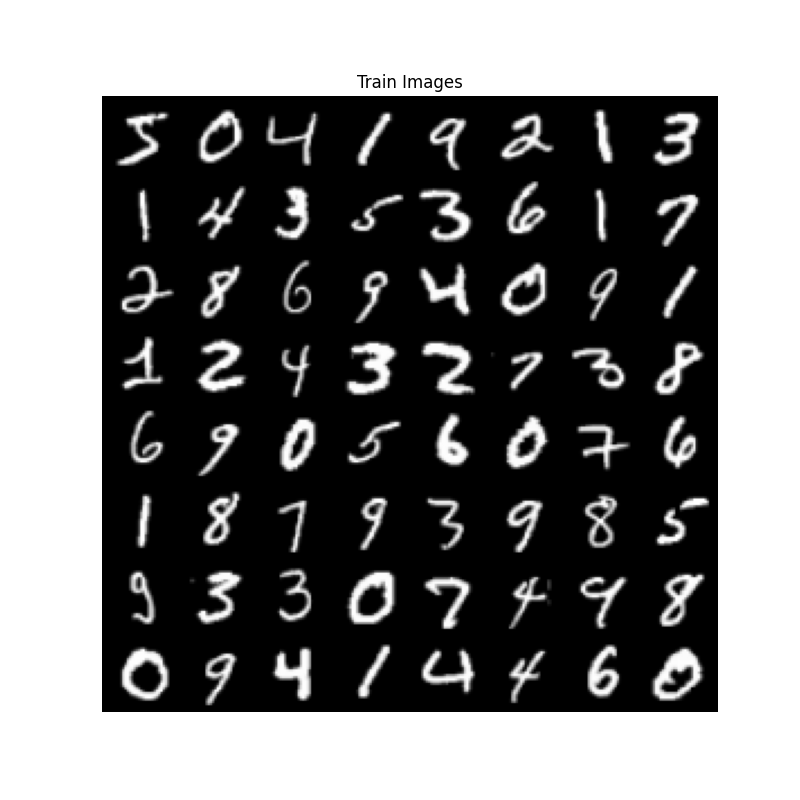
\includegraphics[trim=2.5cm 2cm 2cm 2.5cm ,clip,width=0.3\textwidth]{\toplevelprefix/chapters/chapter5/figs/MNIST_MNIST_train_images_epoch200.png}
%      }   
%      \subfigure[\small CIFAR-10 $\X$]{
%          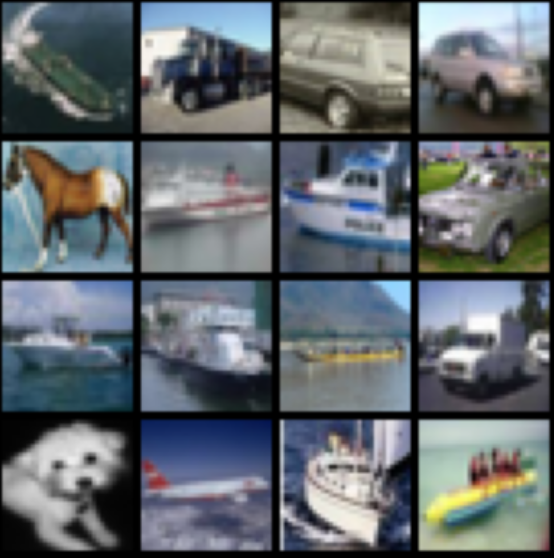
\includegraphics[width=0.3\linewidth]{\toplevelprefix/chapters/chapter5/figs/cifar_input.png}
%      }     
%      \subfigure[\small ImageNet $\X$]{
%          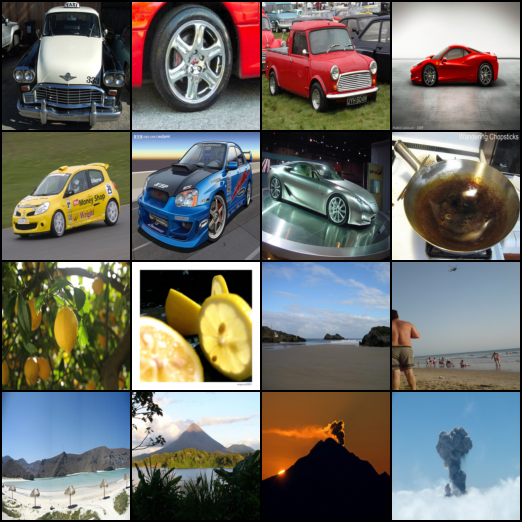
\includegraphics[width=0.3\linewidth]{\toplevelprefix/chapters/chapter5/figs/Imagenet_input.png}
%      }
     
%       \subfigure[\small MNIST $\hat{\X}$]{
%          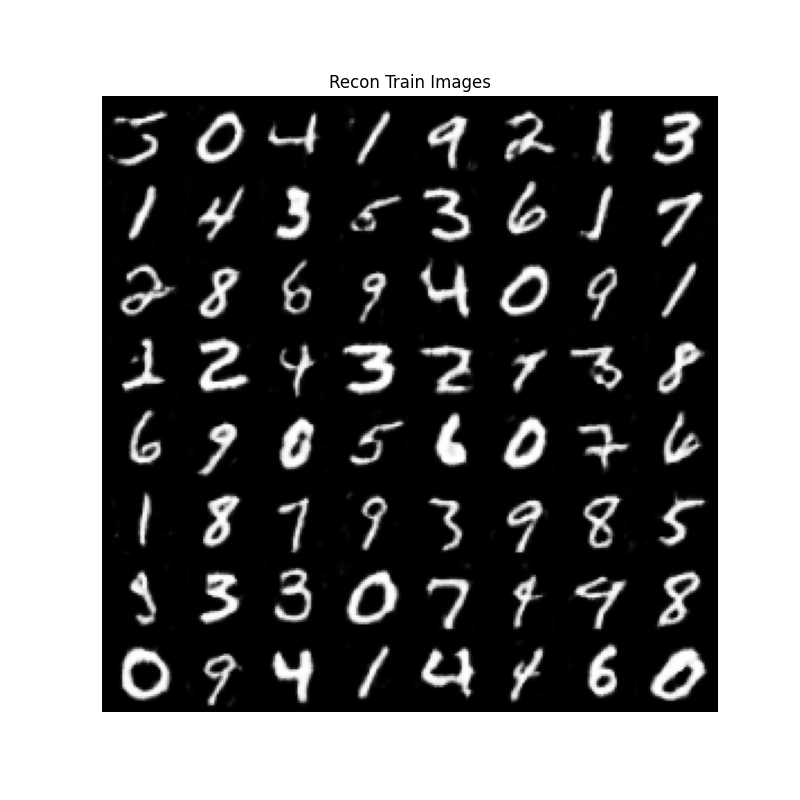
\includegraphics[trim=2.5cm 2cm 2cm 2.5cm ,clip,width=0.3\textwidth]{\toplevelprefix/chapters/chapter5/figs/MNIST_MNIST_train_recon_images_epoch200_multi.png}
%      }
%      \subfigure[\small CIFAR-10 $\hat{\X}$]{
%          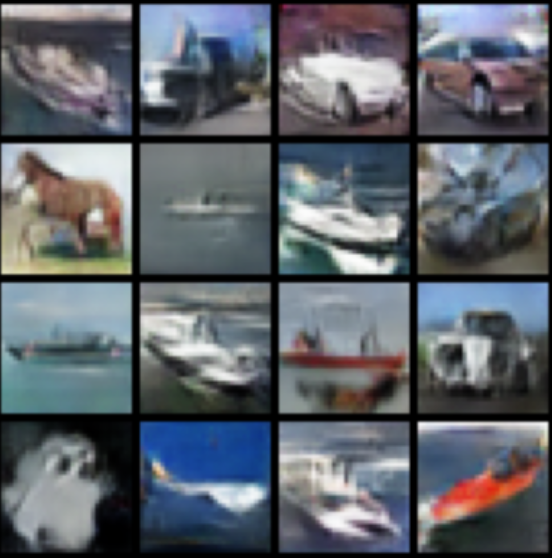
\includegraphics[width=0.3\linewidth]{\toplevelprefix/chapters/chapter5/figs/cifar_reconstruct.png}
%      }
%      \subfigure[\small ImageNet $\hat{\X}$]{
%          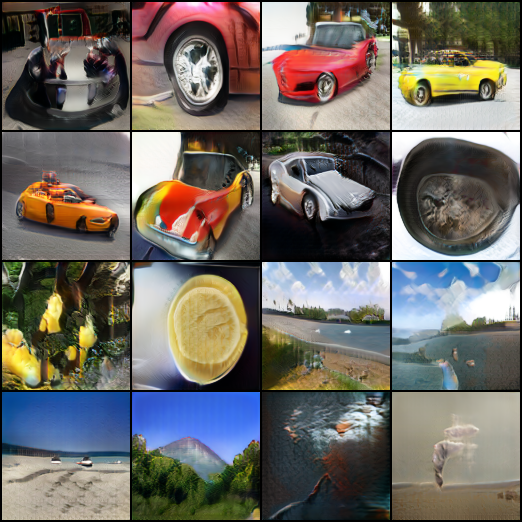
\includegraphics[width=0.3\linewidth]{\toplevelprefix/chapters/chapter5/figs/Imagenet_reconstruct.png}
%     }
%     % \vspace{-0.1in}
%     \caption{Visualizing the auto-encoding property of the learned closed-loop transcription \mbox{($\x \approx \hat{\x} = g\circ f(\x)$)} on MNIST, CIFAR-10, and~ImageNet (zoom in for better visualization).}
%         \label{fig:justifyx=x}
% \end{figure}

\subsection{低维高斯混合模型}
%This subsection provides theoretical justification for \href{https://arxiv.org/abs/2206.09120}{the ideal case when the distribution of $\X $ is already a mixture of low-dimensional subspaces or low-rank  Gaussians (Druv Pai's work)}.

在上面,我们论证了将学习数据分布的问题表述为闭环自编码问题是可能的。我们还从经验上看到,这种方案似乎是有效的。剩下的问题是,这种方案在何时以及为何应该有效。对于具有任意数据分布的最一般情况,回答这个问题是困难的。然而,像往常一样,让我们看看是否能为数据分布是低维子空间或低秩高斯混合的理想情况得出一个严格的论证。对这个重要特例的清晰刻画和理解将为更一般的情况提供启示。\footnote{因为大多数具有低维结构的分布都可以被这类分布很好地近似。}

为此,我们首先假设 \(\vX\) 是根据低维高斯混合分布的,并且 \(\vX\) 的标签(即子空间分配)由 \(\vy\) 给出。然后,我们建立一个极小极大优化问题来学习数据分布,比如说,通过学习将 \(\vX\) 编码为表示 \(\vZ\),这些表示支撑在一个\textit{正交}子空间的混合上,并将 \(\vZ\) 解码回 \(\vX\)。然后,我们想要实现的表示由前面讨论过的信息增益版本最大化,即 \(\Delta R(\vZ) = R(\vZ) - \sum_{k = 1}^{K}\frac{n_{k}}{N}R(\vZ_{k})\),这强制每个类别 \(k\) 的表示 \(\vZ_{k}\) 张成一个与其他类别的支撑子空间正交的子空间。衡量解码一致性的方法,如前所述,由 \(\sum_{k = 1}^{K}\Delta R(\vZ_{k}, \hat{\vZ}_{k})\) 给出,这强制每个类别 \(k\) 的表示 \(\vZ_{k}\) 及其自编码 \(\hat{\vZ}_{k}\) 张成相同的子空间。因此,我们可以建立一个简化的斯塔克伯格博弈:
\begin{equation}\label{eq:ctrl_msp_game}
    \max_{\theta}\min_{\eta}\bc{\Delta R(\vZ(\theta)) + \sum_{j = 1}^{k}\Delta R(\vZ_{k}(\theta), \hat{\vZ}_{k}(\theta, \eta))}
\end{equation}
请注意,这比实践中使用的设置要简单——例如,没有 \(\Delta R(\hat{\vZ})\) 项,而且我们在有类别标签的监督设置下工作(尽管用于证明以下结果的技术很容易扩展到无监督的公式)。此外,表示的一致性仅通过 \(\Delta R\) 在分布层面进行衡量(尽管如果需要,这可以用样本层面的距离度量(如 \(\ell^{2}\) 范数)来代替,并且可以得出等价的结论,\textit{mutatis mutandis})。

在温和的条件下,为了实现所需的编码器和解码器,从一个已经根据相关低维高斯混合分布的数据源 \(\vX\) 中实现 \(\vZ\),我们只需要一个线性编码器和解码器来解耦和白化高斯分布。然后,我们研究 \(\theta\) 和 \(\eta\) 参数化其算子范数受约束的矩阵的情况。

我们想了解在这种设置下学习到的是什么样的最优解。对于这类博弈,其中解码器的最优解仅相对于编码器定义(而不是,特别是,相对于解码器的某些其他内在属性),一个合适的解概念是解码器跟随编码器的\textit{斯塔克伯格均衡}。%\DP{Nika Haghtalab (Berkeley game theory professor) believes very strongly that this should not be called a Stackelberg equilibrium, and the concept of sequential equilibrium is well-defined. Actually, I got a bad grade for my final project because of this naming issue...} 
也就是说,在这样的均衡点,解码器应该优化其目标;同时,编码器应该优化其目标,前提是无论它选择什么,解码器都会选择一个最优响应(这可能会影响编码器目标)。用博弈论的术语来说,这就像解码器\textit{后手}:它在编码器之后选择其权重,并且编码器和解码器都试图根据这一点来优化其目标。通过\textit{交替优化},使用梯度方法学习序贯均衡在计算上是可行的,其中每一方使用不同的学习率。序贯均衡的详细阐述超出了本书的范围,我们在附录 \ref{sec:minimax} 中提供了更多的技术细节。

在这种设置下,我们有以下结果:
\begin{theorem}[\cite{pai2022pursuit}, 节选]\label{thm:ctrl_theory}
    假设 \(\vX\) 分布在一个子空间的混合上。在某些现实但技术性的条件下,\eqref{eq:ctrl_msp_game} 的所有序贯均衡都满足:
    \begin{itemize}
        \item \(\vZ_{k}\) 位于正交子空间上,并且在这些子空间上是各向同性的,即最大化信息增益。
        \item 自编码是自洽的,即对于所有 \(k\),\(\vZ_{k}\) 和 \(\hat{\vZ}_{k}\) 张成的子空间是相同的。
    \end{itemize}
\end{theorem}
如果只有关于数据的几何假设,即没有统计假设,那么这种自洽性的概念是人们所能期望的极限。如果我们假设 \(\vX\) 的列是从一个低秩高斯混合模型中抽取的,那么这个定理的类似版本可以证明 \(\vZ_{k}\) 也是低秩高斯分布,其协方差是各向同性的。%This phenomenon is validated through experiments, see \DP{TODO}.

从本质上讲,这个结果通过子空间上的高斯混合这一简单案例验证了,优化信息增益和自洽性的极小极大博弈可以达到最优解。






\section{持续学习自洽性表示}
\label{sec:continuous}

\subsection{类别增量学习}
\label{sec:class-wise-incremental}
%This subsection shows that the closed-loop architecture is applicable to  \href{https://arxiv.org/abs/2202.05411}{class-wise incremental learning} and it alleviates catastrophic forgetting, probably even with white-box backbone networks. 

正如我们所见,深度神经网络在判别和生成情境中都展示了学习数百甚至数千类物体表示的强大能力。然而,网络通常必须离线训练,同时使用从所有类别中均匀采样的数据。众所周知,当一个(开环)网络在没有旧类别数据的情况下更新以学习新类别时,先前学到的知识将成为{\em 灾难性遗忘}问题的受害者 \cite{McCloskey1989catastrophic}。这在神经科学中被称为稳定性-可塑性困境:确保神经系统能够在学习新环境的同时保留先前环境中的基本知识的挑战 \cite{Grossberg1987CompetitiveLF}。

相比之下,自然神经系统(例如动物大脑)似乎完全没有遭受这种灾难性遗忘。它们能够在学习新物体的同时,保留对先前学习过的物体的记忆。这种能力,无论是对于自然还是人工神经系统,通常被称为{\em 增量学习、持续学习、序贯学习}或{\em 终身学习}~ \cite{controlled-forgetting}。



尽管许多最近的工作强调了如何以更灵活的方式训练人工神经系统,但现有解决人工神经网络稳定性-可塑性困境的最强努力通常需要存储原始样本 \cite{icarl,chaudhry2019tiny} 或提供外部机制 \cite{EWC}。原始样本,特别是在像图像这样的高维输入情况下,成本高昂且难以扩展,而外部机制——通常包括用于生成式回放的次级网络和表示空间、网络资源的增量分配、网络复制或对网络已使用和未使用部分的明确隔离——需要启发式方法并产生隐藏成本。


在这里,我们感兴趣的是一种类似于自然的增量学习设置。它通过两个关键特性来应对现有实践。
\begin{enumerate}
    \item 第一个是它应该是\emph{基于记忆的。} 在学习新类别时,没有旧类别的原始样本可用于与新数据一起训练网络。这意味着必须依赖于为旧类别学习到的紧凑且结构化的“记忆”,例如旧类别的增量学习的生成式表示,以及相关的编码和解码映射~\cite{fearnet}。
    \item 第二个是它应该是\emph{自包含的。} 增量学习在具有固定容量的单个神经系统中,在一个共同的表示空间中进行。最小化遗忘的能力是通过优化一个整体学习目标来实现的,而不需要外部网络、架构修改或资源分配机制。
\end{enumerate}

不同类别特征的非相干线性结构与动物大脑颞下皮层中物体编码的方式非常相似 \cite{Chang-Cell-2017,Bao2020AMO}。闭环转录 $\X \rightarrow \Z \rightarrow \hat{\X} \rightarrow \hat{\Z}$ 也类似于普遍假设的记忆形成机制 \cite{2020Vandeven,Josselyn2020MemoryER}。这就引出了一个问题:既然大脑中的记忆是以增量方式形成的,那么上述闭环转录框架是否也支持增量学习?

\paragraph{LDR 记忆采样与回放。} LDR 的简单线性{\em 结构}使其特别适合增量学习:每个先前学习过的类别的特征 $\Z_j$ 的分布可以由特征空间中的一个主子空间 $\mathcal{S}_j$ 明确而简洁地表示。为了保留旧类别 $j$ 的记忆,我们只需要在学习新类别时保留该子空间。为此,我们只需沿着其前 $r$ 个主成分在该子空间上采样 $m$ 个代表性的原型特征,并将这些特征表示为 $\Z_{j,old}$。由于 LDR 的简单线性结构,我们可以在学习类别 $j$ 后,通过计算 $\Z_{j,old}$ 的均值和协方差来从 $\Z_{j,old}$ 中采样。所需的存储空间极小,因为我们只需要存储均值和协方差,并根据需要从中采样。假设到目前为止总共学习了 $t$ 个旧类别。如果在学习新类别时,所有这些类别的原型特征(表示为 $\Z_{old} \doteq [\Z^1_{old},\ldots, \Z^t_{old}]$)都能被保留,那么代表过去记忆的子空间 $\{\mathcal{S}_j\}_{j=1}^t$ 也将被保留。关于采样和计算均值与协方差的更多细节可以在 \cite{tong2023incremental} 的工作中找到。
%Appendix \ref{algorithm:prototype} and Appendix~\ref{algorithm:Sampling}

\begin{figure*}[t]
\centering
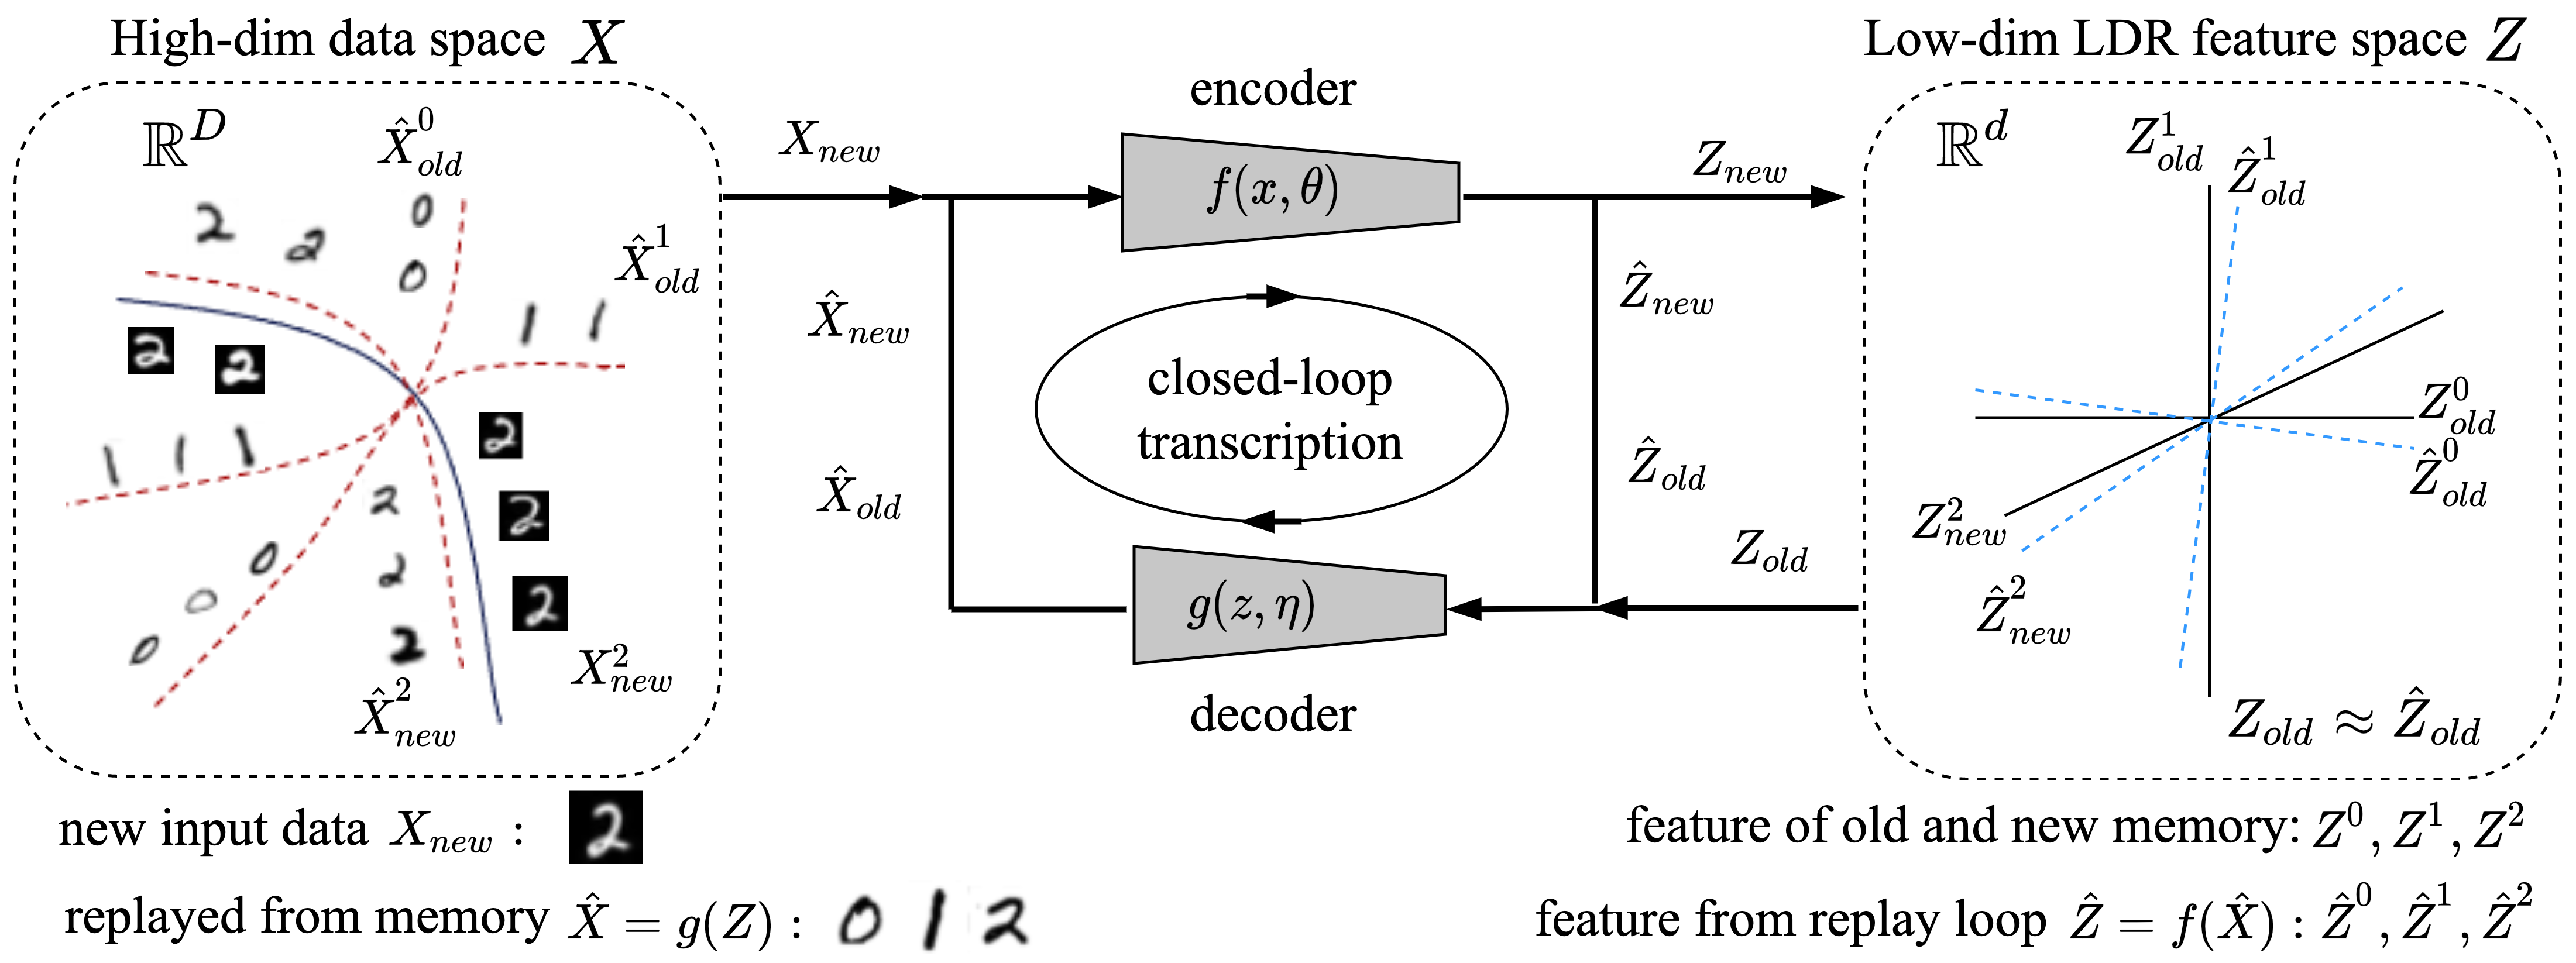
\includegraphics[width=0.9\textwidth]{\toplevelprefix/chapters/chapter5/figs/framework-v7.png}
\caption{\textbf{我们基于闭环转录的增量学习的整体框架},用于结构化的 LDR 记忆。只需要一个单一的、完全自包含的编码-解码网络:对于一个新的数据类别 $\X_{new}$,一个新的 LDR 记忆 $\Z_{new}$ 通过编码器和解码器之间的极小极大博弈增量学习,同时受限于过去类别的旧记忆 $\Z_{old}$ 通过闭环转录(或回放)保持不变的约束:$\Z_{old} \approx \hat{\Z}_{old} = f(g(\Z_{old}))$。
\vspace{-0.2in}}
\label{fig:framework}
\end{figure*}

\paragraph{带有旧记忆约束的增量学习 LDR。} 
请注意,通过学习到的自编码 \eqref{eqn:autoencoding-ch6},人们可以回放并使用与记忆特征相关的图像,比如 $\hat\X_{old} = g(\Z_{old}, \eta)$,以在学习新类别时避免遗忘。这通常是生成模型在先前的增量学习方法中被使用的方式。然而,在闭环框架下,从特征中明确地回放图像是不必要的。过去的记忆可以通过完全在特征本身上进行优化来有效地保留。

考虑增量学习一个新类别物体的任务。\footnote{当然,也可以考虑更一般的情况,即任务包含一小批新类别,而无需进行重大修改。} 我们将相应的新样本集表示为 $\X_{new}$。$\X_{new}$ 的特征表示为 $\Z_{new}(\theta) = f(\X_{new}, \theta)$。我们将它们与旧类别的原型特征 $\Z_{old}$ 连接起来,形成 $\Z = [\Z_{new}(\theta), \Z_{old}]$。我们将所有特征回放的图像表示为 $\hat{\X} = [{\hat{\X}_{new}(\theta,\eta)}, {\hat{\X}_{old}(\eta)}]$,尽管我们实际上不需要计算或显式地使用它们。我们只需要回放图像的特征,表示为 $\hat{\Z} = f(\hat{\X}, \theta) =  [{\hat{\Z}_{new}(\theta,\eta)}, {\hat{\Z}_{old}(\theta,\eta)}]$。


与多类别 CTRL 目标 \eqref{eq:MCR2-GAN-objective} 的动机相呼应,我们希望新类别 $\Z_{new}$ 的特征与所有旧类别 $\Z_{old}$ 的特征不相关。由于 $\Z_{new}$ 是唯一需要学习其特征的新类别,目标 \eqref{eq:MCR2-GAN-objective} 简化为 $k=1$ 的情况:
\begin{equation}
\min_\eta \max_\theta \Delta{R(\Z)}+\Delta{R(\hat{\Z})}+\Delta{R(\Z_{new},\hat{\Z}_{new})}.
\label{eqn:unconstrained-minimax}
% \vspace{-2mm}
\end{equation}
然而,当我们更新网络参数 $(\theta, \eta)$ 以优化新类别的特征时,更新后的映射 $f$ 和 $g$ 也会改变旧类别的特征。因此,为了最小化旧类别表示的失真,我们可以尝试强制 $\mbox{Cov}(\Z_{j,old}) = \mbox{Cov}(\hat{\Z}_{j,old})$。换句话说,在学习新类别时,我们强制旧类别的记忆通过转录循环保持“自洽”:
\begin{equation}
\Z_{old} \xrightarrow{\hspace{2mm} g(\z,\eta) \hspace{2mm}} \hat \X_{old} \xrightarrow{\hspace{2mm} f(\x, \theta)\hspace{2mm}} \ \hat \Z_{old}.
\end{equation}
在数学上,这等价于设置
$$\Delta R(\Z_{old},\hat{\Z}_{old}) \doteq  \sum_{j=1}^t \Delta R(\Z_{j,old},\hat{\Z}_{j,old}) = 0.$$  
因此,上述极小极大程序 \eqref{eqn:unconstrained-minimax} 被修正为一个{\em 约束}极小极大博弈,我们称之为{\em 增量闭环转录} (i-CTRL)。
这个博弈的目标与标准的多类别 CTRL 目标 \eqref{eq:MCR2-GAN-objective} 相同,但只增加了一个额外的约束:
%\begin{small}
\begin{eqnarray}
\min_\eta \max_\theta  &&\Delta{R(\Z)}+\Delta{R(\hat{\Z})}+\Delta{R(\Z_{new},\hat{\Z}_{new})} \nonumber\\
&& \mbox{约束条件} \quad  \Delta R(\Z_{old},\hat{\Z}_{old}) = 0.
\label{eqn:constrained-minimax}
\end{eqnarray}
%\end{small}
% This is equivalent to the multi-class CTRL objective \eqref{eq:MCR2-GAN-objective} with an additional constraint $\Delta R(\Z_{old},\hat{\Z}_{old}) = 0$. % is the only thing that we need to modify the original formulation. 

在实践中,这个约束极小极大程序可以通过在编码器 $f(\cdot, \theta)$ 和解码器 $g(\cdot, \eta)$ 之间进行{\em 交替}最小化和最大化来求解,如下所示:
%\begin{small}
\begin{eqnarray}
&\max_\theta  &\Delta{R(\Z)}\!+\!\Delta{R(\hat{\Z})}\!+\!\lambda\cdot  \Delta{R(\Z_{new},\hat{\Z}_{new})} - \gamma\cdot \Delta{R(\Z_{old},\hat{\Z}_{old})}, \label{eqn:relaxed-max}\\ 
&\min_\eta &\Delta{R(\Z)}\!+\!\Delta{R(\hat{\Z})}\!+\!\lambda\cdot \Delta{R(\Z_{new},\hat{\Z}_{new})} + \gamma\cdot \Delta{R(\Z_{old},\hat{\Z}_{old})}; \label{eqn:relaxed-min}
\end{eqnarray}
%\end{small}
其中 \eqref{eqn:constrained-minimax} 中的约束 $\Delta R(\Z_{old},\hat{\Z}_{old}) = 0$ 已被转换(并松弛)为一个带有相应系数 $\gamma$ 和符号的拉格朗日项。我们还引入了另一个系数 $\lambda$ 用于加权与新数据相关的编码率降低项。% to balance between old and new classes.
%More algorithmic details are given in Appendix \ref{app:algorithm}.



\paragraph{通过增量复习实现联合最优记忆。} 
正如我们将看到的,上述约束极小极大程序已经可以在增量学习中达到最先进的性能。然而,为{\em 所有类别}开发一个最优记忆不能仅仅依赖于优雅的遗忘。即使对于人类来说,如果一个物体类别只学习一次,我们应该预料到,随着我们继续学习其他新事物,学到的记忆会逐渐淡忘,除非通过复习旧的物体类别来巩固记忆。

为了模拟记忆形成的这个阶段,在增量学习完整个数据集后,我们可以回头再次复习所有类别,一次一个类别。我们将遍历所有类别一次称为一个复习“周期”。\footnote{以区别于传统联合学习设置中使用的术语“轮次”。} 如果需要,可以进行多个复习周期。复习可以改善学到的(LDR)记忆是意料之中的。但有些令人惊讶的是,闭环框架甚至允许我们以“{类别无监督}”的方式进行复习:当复习一个旧类别(比如 $\X_j$)的数据时,系统不需要类别标签,可以简单地将 $\X_j$ 视为一个新类别 $\X_{new}$。也就是说,系统优化相同的约束极小极大程序 \eqref{eqn:constrained-minimax} 而无需任何修改;在系统优化后,可以识别出新学习到的由 $\Z_{new}$ 张成的子空间,并用它来替换或合并旧的子空间 $\mathcal{S}_j$。正如我们的实验所示,这种类别无监督的增量复习过程可以逐渐提高 LDR 记忆的判别和生成性能,最终收敛到联合学习记忆的性能。

\paragraph{实验验证。}
我们在以下数据集上展示了一些实验结果:MNIST \cite{lecun1998gradient} 和 CIFAR-10 \cite{krizhevsky2014cifar}。所有实验都是在更具挑战性的 class-IL 设置下进行的。对于 MNIST 和 CIFAR-10,10 个类别被分成 5 个任务,每个任务 2 个类别,或者 10 个任务,每个任务 1 个类别。对于编码器 $f$ 和解码器 $g$,我们采用了一个非常简单的网络架构,修改自 DCGAN \cite{radford2016unsupervised},它仅仅是一个{\em 四层}卷积网络。这里我们只展示一些定性的视觉结果,更多的实验和分析可以在 \cite{tong2023incremental} 的工作中找到。

\paragraph{可视化自编码属性。}
我们首先定性地可视化一些代表性的图像 $\X$ 和相应的回放图像 $\hat{\X}$ 在 MNIST 和 CIFAR-10 上的表现。模型是在数据集被分成 5 个任务的情况下增量学习的。结果如图 \ref{fig:justifyx=x} 所示,我们观察到重构的 $\hat{\X}$ 保留了 $\X$ 的主要视觉特征,包括形状和纹理。对于像 MNIST 这样更简单的数据集,回放的 $\hat{\X}$ 几乎与输入的 $\X$ 相同!考虑到以下几点,这是相当了不起的:(1)我们的方法不像大多数自编码方法那样明确强制单个样本的 $\hat{\x} \approx \x$;(2)在增量学习完所有类别后,生成器没有忘记如何生成早期学习的数字,如 0、1、2。对于像 CIFAR-10 这样更复杂的数据集,我们也展示了良好的视觉质量,忠实地捕捉了每张图像的精髓。

\begin{figure}[t]
    \begin{subfigure}[t]{0.20\textwidth}
        \centering
        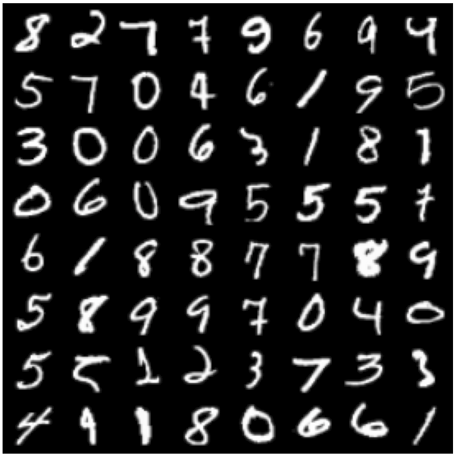
\includegraphics[width=\textwidth]{\toplevelprefix/chapters/chapter5/figs/mnist_x.png}
        \caption{MNIST $\X$}
    \end{subfigure}
    \hfill
    \begin{subfigure}[t]{0.20\textwidth}
        \centering
        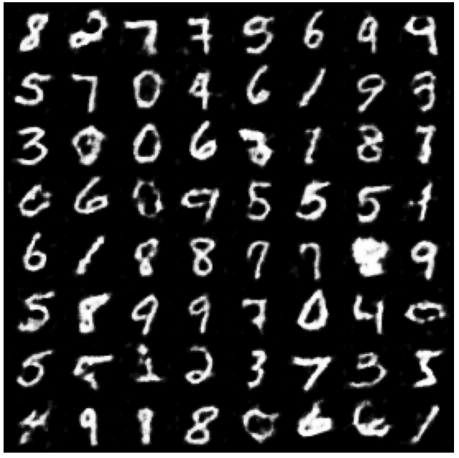
\includegraphics[width=\textwidth]{\toplevelprefix/chapters/chapter5/figs/mnist_recon_x.png}
        \caption{MNIST $\hat{\X}$}
    \end{subfigure}
    \hfill
    \begin{subfigure}[t]{0.20\textwidth}
        \centering
        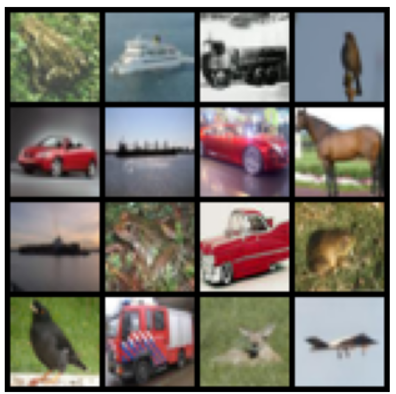
\includegraphics[width=\textwidth]{\toplevelprefix/chapters/chapter5/figs/cifar10_x.png}
        \caption{CIFAR-10 $\X$}
    \end{subfigure}
    \hfill
    \begin{subfigure}[t]{0.20\textwidth}
        \centering
        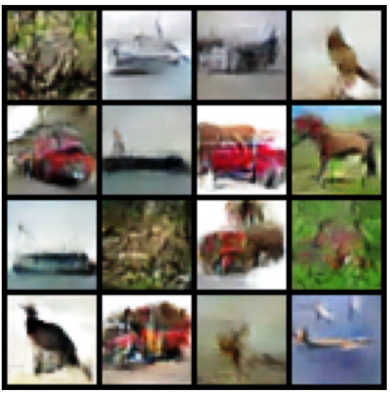
\includegraphics[width=\textwidth]{\toplevelprefix/chapters/chapter5/figs/cifar10_x_recon.png}
        \caption{CIFAR-10 $\hat{\X}$}
    \end{subfigure}
    \caption{\small 可视化学习到的自编码属性($\hat{\X} = g\circ f(\X)$)。}
        % \label{fig:justifyx=x}
\end{figure}


\paragraph{学习到的特征的主子空间。}
大多数基于生成式记忆的方法利用自编码器、VAE 或 GAN 进行回放。每个类别的学习特征 $\Z_j$ 的结构或分布在特征空间中是不清楚的。另一方面,LDR 记忆的特征 $\Z_j$ 具有清晰的线性结构。图 \ref{fig:cifar_10_pca_sampling_main} 可视化了所有学习特征之间的相关性 $|\Z^\top\Z|$,其中我们观察到两个数据集都具有清晰的块对角模式。\footnote{请注意,这些模式与颞下皮层不同区域对物体类别的响应谱的相似性矩阵非常相似,如 \cite{Bao2020AMO} 的扩展数据图3所示。} 这表明不同类别 $\Z_j$ 的特征确实位于相互不相关的子空间上。因此,每个类别的特征可以很好地被建模为特征空间中的一个主子空间。%A more precise measure of affinity among those subspaces can be found in Appendix~\ref{app:analysis}.

\begin{figure}[tb]
\centering
\includegraphics[height=4.1cm]{\toplevelprefix/chapters/chapter5/figs/Heatmap_MNIST.jpg}  \includegraphics[height=4cm]{\toplevelprefix/chapters/chapter5/figs/Heatmap_CIFAR10.png}
\caption{\small MNIST(左)和 CIFAR-10(右)特征空间中 $|\Z^\top \Z|$ 的块对角结构。}
\label{fig:cifar_10_pca_sampling_main}
\end{figure}

% \begin{figure}[t]
% \centering
%  \subfigure[MNIST]{
%      \includegraphics[width=0.20\textwidth]{Fig/Experiment/MNIST/Heatmap_MNIST.jpg}
%  }
%  \hspace{5mm}
%   \subfigure[CIFAR-10]{
%      \includegraphics[width=0.20\textwidth]{Fig/Experiment/CIFAR10/Heatmap_CIFAR10.png}
%  }
%  \vspace{-0.18in}
%  \caption{\small Block diagonal structure of $|\Z^\top \Z|$ in the feature space for MNIST (left) and CIFAR-10 (right). \vspace{-5mm}}
%  \label{fig:cifar_10_pca_sampling_main}
% \end{figure}


\paragraph{从主成分采样的回放图像。}
由于每个类别的特征都可以被建模为一个主子空间,我们进一步可视化了这些子空间中的各个主成分。图 \ref{fig:pca_sampling_main} 分别显示了在 MNIST 和 CIFAR-10 上,从不同类别的前4个主成分采样的特征回放的图像。每一行代表沿一个主成分的样本,它们清晰地显示出相似的视觉特征,但与其他行的特征有明显不同。我们看到,在学习完所有剩余类别后,模型仍然记得‘4’的不同姿态。对于 CIFAR-10,增量学习的记忆记得马和船的代表性姿态和形状。

\begin{figure}[t]
    \begin{subfigure}[t]{0.20\textwidth}
        \centering
        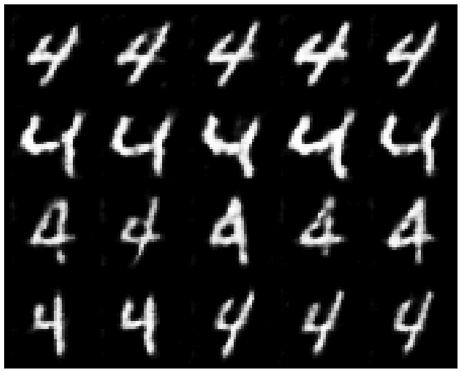
\includegraphics[width=\textwidth]{\toplevelprefix/chapters/chapter5/figs/mnist_4.png}
        \caption{‘4’的采样 $\hat{\x}_{old}$}
    \end{subfigure}
    \hfill
    \begin{subfigure}[t]{0.20\textwidth}
        \centering
        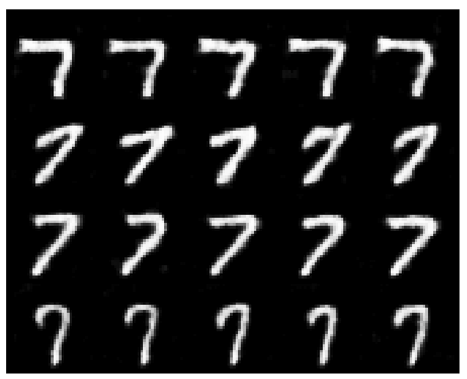
\includegraphics[width=\textwidth]{\toplevelprefix/chapters/chapter5/figs/mnist_7.png}
        \caption{‘7’的采样 $\hat{\x}_{old}$}
    \end{subfigure}
    \hfill
    \begin{subfigure}[t]{0.20\textwidth}
        \centering
        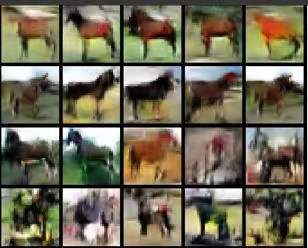
\includegraphics[width=\textwidth]{\toplevelprefix/chapters/chapter5/figs/horse_z.jpg}
        \caption{‘马’的采样 $\hat{\x}_{old}$}
    \end{subfigure}
    \hfill
    \begin{subfigure}[t]{0.20\textwidth}
        \centering
        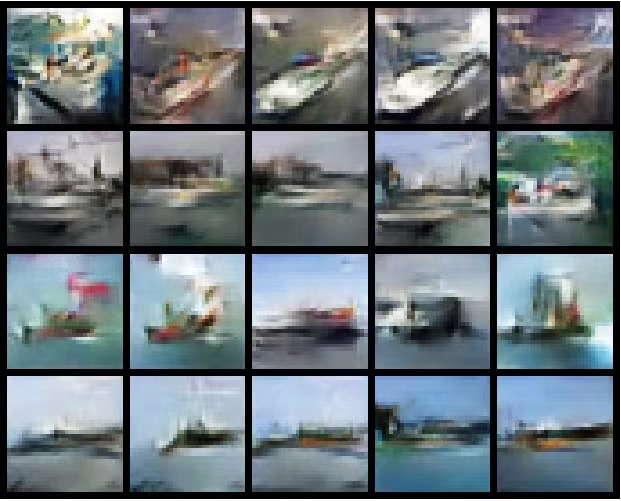
\includegraphics[width=\textwidth]{\toplevelprefix/chapters/chapter5/figs/ship_z.jpg}
        \caption{‘船’的采样 $\hat{\x}_{old}$}
    \end{subfigure}
    \caption{\small 从与 {MNIST}(类别‘4’和类别‘7’)和 {CIFAR-10}(类别‘马’和‘船’)学习特征的(前4个)主成分距离最近的 $\z$ 重构的 5 个 $\hat \x=g(\z)$ 的可视化。}
    \label{fig:pca_sampling_main}
\end{figure}

% \begin{figure}[t]
% \centering
%  \subfigure[sampled $\hat{\x}_{old}$ of `4']{
%      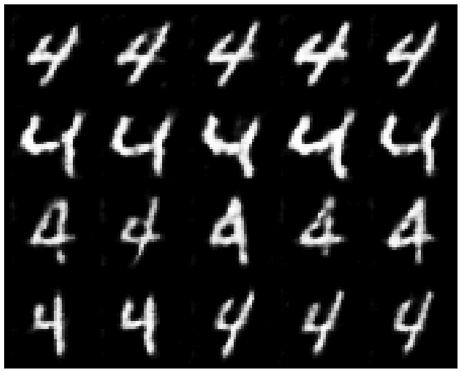
\includegraphics[width=0.2\textwidth]{\toplevelprefix/chapters/chapter5/figs/mnist_4.png}
%  }
%   \subfigure[sampled $\hat{\x}_{old}$ of `7']{
%      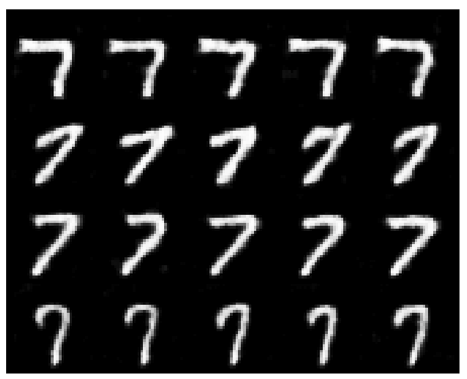
\includegraphics[width=0.2\textwidth]{\toplevelprefix/chapters/chapter5/figs/mnist_7.png}
%  }
%   \subfigure[\footnotesize sampled $\hat{\x}_{old}$ of  `horse']{
%      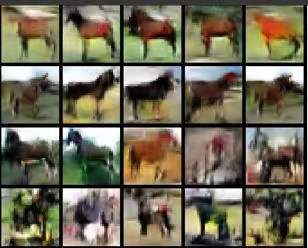
\includegraphics[width=0.2\textwidth]{\toplevelprefix/chapters/chapter5/figs/horse_z.jpg}
%  }
%   \subfigure[sampled $\hat{\x}_{old}$ of `ship']{
%      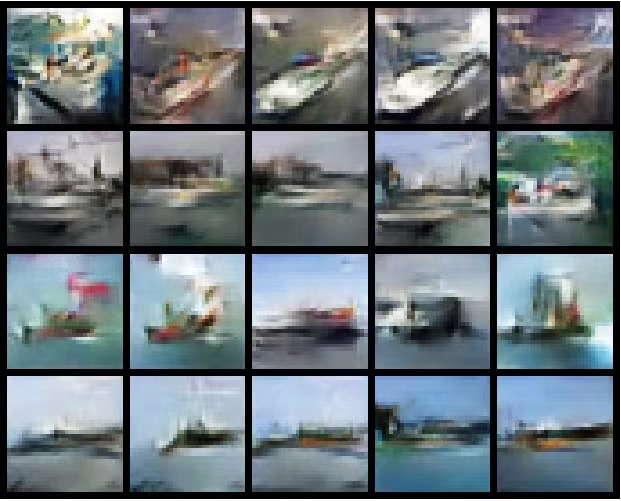
\includegraphics[width=0.2\textwidth]{\toplevelprefix/chapters/chapter5/figs/ship_z.jpg}
%  }
%  \caption{\small Visualization of 5 reconstructed $\hat \x=g(\z)$ from $\z$'s with the closest distance to (top-4) principal components of learned features for {MNIST} (class ‘4’ and class ‘7’) and {CIFAR-10} (class ‘horse’ and  ‘ship’).}
%  \label{fig:pca_sampling_main}
% \end{figure}


\paragraph{增量复习的有效性。}
我们验证了增量学习的 LDR 记忆如何通过前面描述的无监督增量复习阶段得到进一步巩固。实验在 CIFAR-10 上进行,共 10 个步骤。图 \ref{fig:memory_review} 左侧显示了在增量学习完所有十个类别后,第一个类别‘飞机’的回放图像,这些图像是沿着前3个主成分采样的——每两行(16 张图像)是沿着一个主方向。它们的视觉质量仍然非常好——几乎没有观察到遗忘。右图显示了复习完第一个类别一次后的回放图像。我们注意到复习后视觉质量有显著提高,并且子空间中特征的主成分开始对应于同一类别内明显不同的视觉属性。

\begin{figure}
\centering
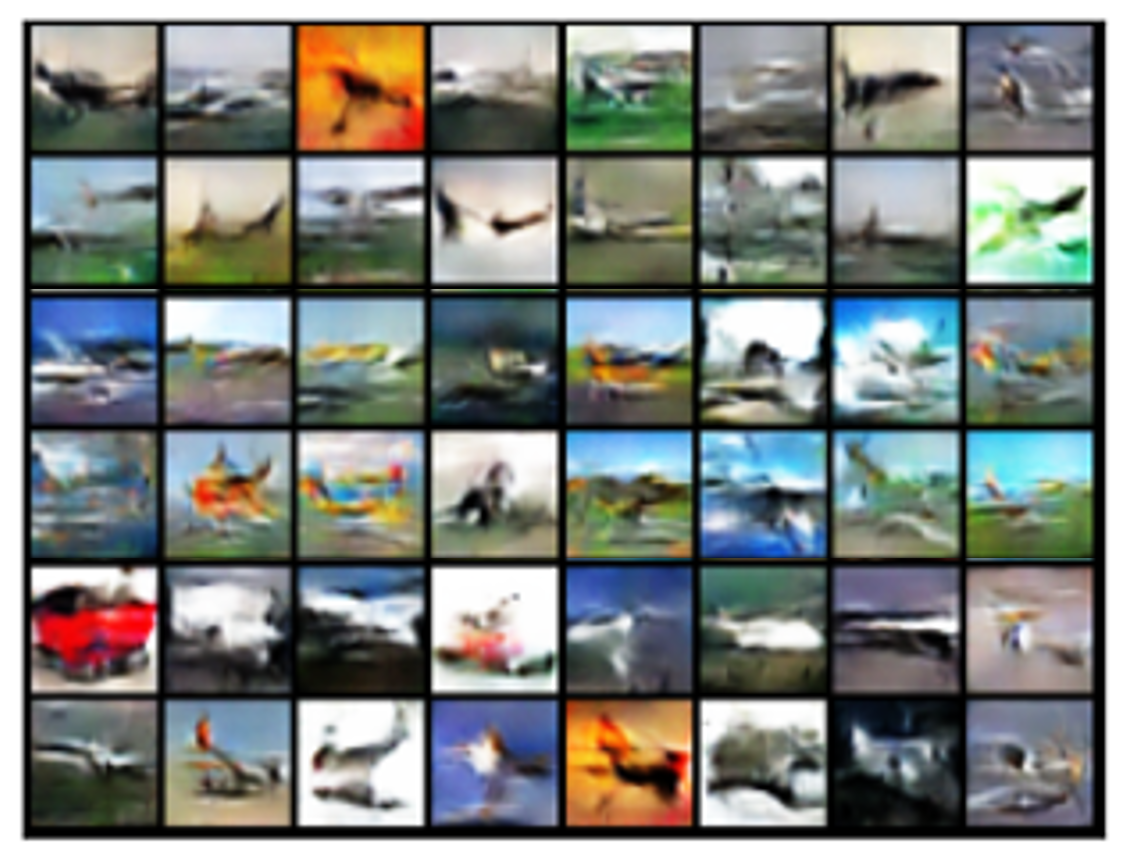
\includegraphics[width=0.41\textwidth]{\toplevelprefix/chapters/chapter5/figs/memory_before_review_clip.png}
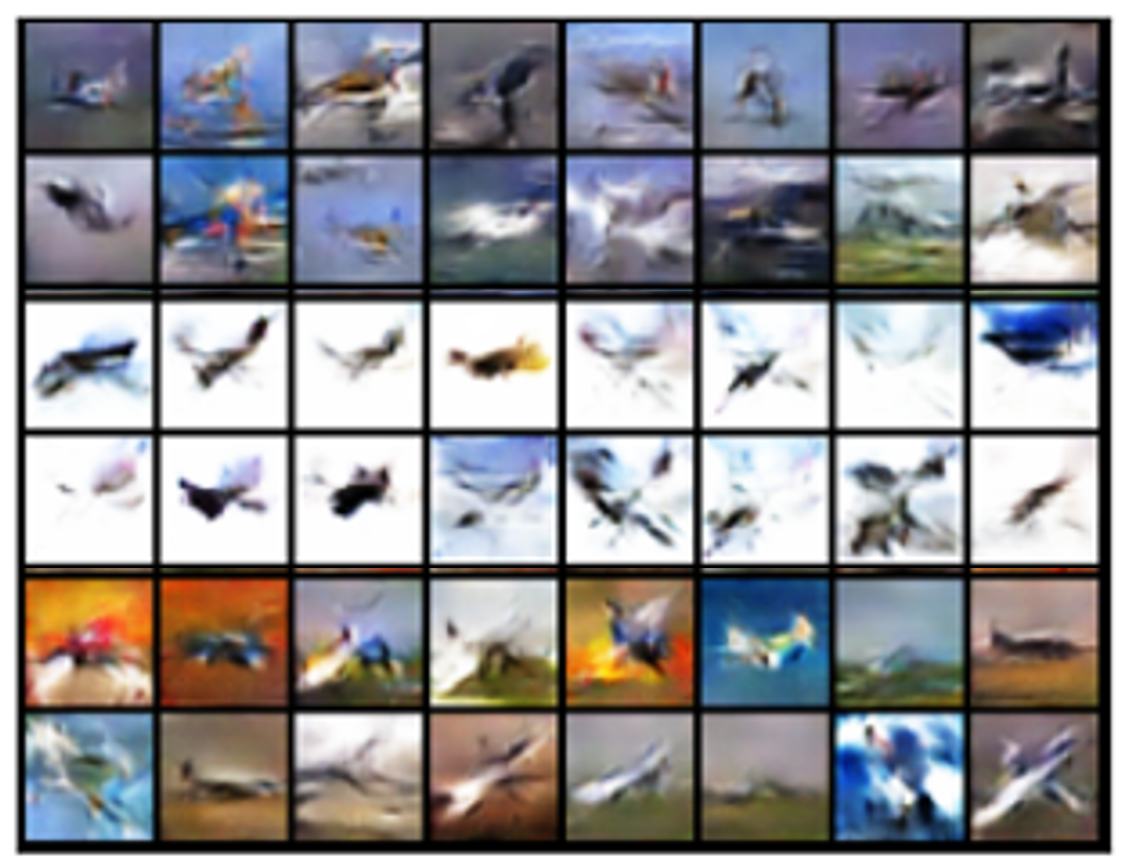
\includegraphics[width=0.4\textwidth]{\toplevelprefix/chapters/chapter5/figs/memory_after_review_clip.png}
 \caption{\small CIFAR-10 中类别 1-‘飞机’的回放图像 $\hat{\x}_{old}$ 的可视化,在一次复习周期之前(左)和之后(右)。} 
\label{fig:memory_review}
\end{figure}


\subsection{样本级持续无监督学习}
\label{sec:sample-wise-incremental}
%This subsection shows that the closed-loop architecture is applicable to \href{https://arxiv.org/abs/2210.16782}{sample-wise continuous learning}, probably even with white-box backbone networks.

正如我们所知,即使没有类别信息,闭环 CTRL 公式也可以通过 CTRL-Binary 程序学习一个不错的自编码:
\begin{align}
      \max_\theta \min_\eta \quad \Delta R(\Z, \hat{\Z}) 
 \label{eqn:CTRL-Binary}
\end{align}
然而,请注意 \eqref{eqn:CTRL-Binary} 在实践中是有限的,因为它只在分布层面对齐数据集 $\X$ 和再生的 $\hat \X$。
不能保证对于每个样本 $\x$ 都会接近解码后的 $\hat \x = g(f(\x))$。

\paragraph{无监督转录的样本级约束。} 
\label{sec:constraints}
为了改善在无监督设置下学习到的表示的判别和生成特性,我们为上述 CTRL-Binary 极小极大博弈 \eqref{eqn:CTRL-Binary} 提出了两种额外的机制。为简单和统一,这里将它们表述为关于编码率降低度量的等式约束,但在实践中,它们可以在优化过程中被软性地强制执行。

\paragraph{通过闭环转录实现样本级自洽性。} 
首先,为了解决 CTRL-Binary 不学习样本级一致自编码的问题,我们需要促进每个样本的 $\hat \x$ 接近 $\x$。在 CTRL 框架中,这可以通过强制它们对应的特征 $\z=f(\x)$ 和 $\hat \z = f(\hat \x)$ 接近来实现。
为了促进样本级自洽性,即 $\hat{\x} = g(f(\x))$ 接近 $\x$,我们希望对于所有 $N$ 个样本,$\z$ 和 $\hat{\z}$ 之间的距离为零或很小。
这个距离可以用编码率降低来衡量:
\begin{align}
\sum_{i\in N} \Delta R(\z^i,\hat{\z}^i) = 0.
\label{eqn:sample-self-consistency}\vspace{-2mm}
\end{align}
请注意,这再次避免了在图像空间中测量差异。

\paragraph{通过压缩增强样本实现自监督。} 
由于我们在无监督设置中不知道样本之间的任何类别标签信息,我们能做的最好的事情就是将每个样本及其增强(例如通过平移、旋转、遮挡等)视为一个“类别”——这是几乎所有自监督学习方法背后的基本思想。在编码率降低框架中,压缩每个样本及其增强的特征是很自然的。在这项工作中,我们采用 SimCLR \cite{chen2020simple} 中的标准变换,并将这种变换表示为 $\tau$。我们将每个增强样本表示为 $\x_a = \tau(\x)$,其对应的特征表示为 $\z_a = f(\x_a, \theta)$。出于判别目的,我们希望分类器对这种变换是{\em 不变的}。因此,很自然地要求所有增强的特征 $\z_a$ 与原始样本 $\x$ 的特征 $\z$ 相同。这等价于要求对于所有 $N$ 个样本,$\z$ 和 $\z_a$ 之间的距离(再次用编码率降低来衡量)为零(或很小):
\begin{align}
\sum_{i\in N} \Delta R(\z^i,\z_{a}^i) = 0.
\label{eqn:sample-compression}\vspace{-3mm}
\end{align}


\paragraph{通过闭环转录进行无监督表示学习。} 
到目前为止,我们知道 CTRL-Binary 目标 $\Delta R(\Z, \hat{\Z})$ 在 \eqref{eqn:CTRL-Binary} 中有助于对齐分布,而样本级自洽性 \eqref{eqn:sample-self-consistency} 和样本级增强 \eqref{eqn:sample-compression} 有助于对齐和压缩与每个样本相关的特征。除了一致性,我们还希望学习到的表示对于不同样本(这里视为不同的“类别”)具有最大的判别性。请注意,编码率失真项 $R(\Z)$ 衡量了所有特征的编码率(因此是体积)。%It has been observed in \cite{li2022neural} that by maximizing this term, learned features expand and hence become more discriminative. 

\paragraph{无监督 CTRL。} 将这些元素放在一起,我们提出通过以下约束极小极大程序来学习表示,我们称之为{\em 无监督 CTRL} (u-CTRL):
\begin{align}
      \max_\theta \min_\eta  \quad & R(\Z) + \Delta R(\Z, \hat{\Z}) \label{eqn:constrained_maxmin}\\
 \mbox{约束条件} \quad & \sum_{i\in N} \Delta R(\z^i, \hat{\z}^i) = 0, \;\; \mbox{和} \;\; \sum_{i\in N} \Delta R(\z^i, \z_{a}^i) = 0. \nonumber
\end{align}
图 \ref{fig:framework-uCTRL} 说明了与此程序相关的闭环系统的整体架构。
\begin{figure}[t]
\centering
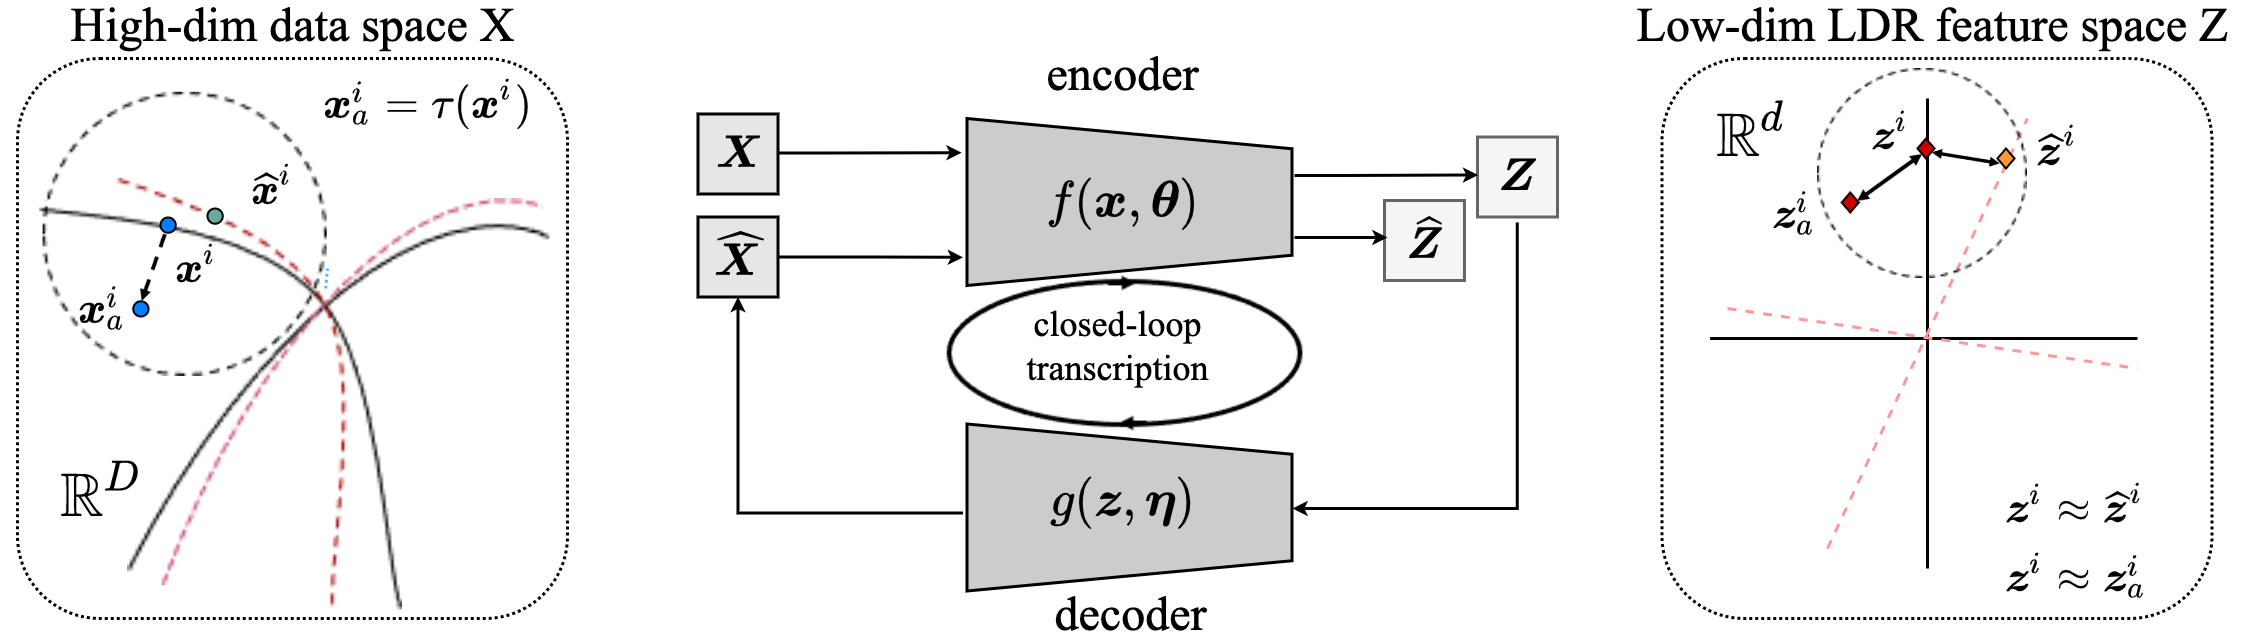
\includegraphics[width=0.98\textwidth]{\toplevelprefix/chapters/chapter5/figs/uCTRLv3.png}
\caption{\textbf{用于无监督学习的闭环转录的整体框架。} 在 Binary-CTRL 方法上施加了两个额外的约束:1) 样本级特征 $\z^i$ 和 $\hat{\z}^i$ 的自洽性,即 $\z^i \approx \hat{\z}^i$;2) 增强样本 $\z^i$ 和 $\z_{a}^i$ 特征之间的不变性/相似性,即 $\z^i \approx \z_{a}^i=f(\tau(\x^i), \theta)$,其中 $\x^i_a=\tau(\x^i)$ 是样本 $\x^i$ 通过某个变换 $\tau(\cdot)$ 的增强。}
\label{fig:framework-uCTRL}
\end{figure}

在实践中,上述程序可以通过在编码器 $f(\cdot,\theta)$ 和解码器 $g(\cdot,\eta)$ 之间交替进行最大化和最小化来优化。我们采用以下在实践中效果良好的优化策略,该策略用于所有后续在真实图像数据集上的实验:
\vspace{-1mm}
\begin{align}
  &  \max_{\theta}\; R(\Z) + \Delta{R(\Z, \hat{\Z})-\lambda_{1}\sum_{i\in N} \Delta R(\z^i, \z_{a}^i)} -\lambda_{2}\sum_{i\in N} \Delta R(\z^i, \hat{\z}^i) \label{eqn:constrained_max}; \\
% \end{align}
% \begin{align}
   & \min_{\eta}\; R(\Z) + \Delta{R(\Z, \hat{\Z})+\lambda_{1}\sum_{i\in N} \Delta R(\z^i, \z_{a}^i)+ \lambda_{2}\sum_{i\in N} \Delta R(\z^i, \hat{\z}^i)} \label{eqn:constrained_min}, 
\end{align}
其中 \eqref{eqn:constrained_maxmin} 中的约束 $\sum_{i\in N} \Delta R(\z^i, \hat{\z}^i) = 0$ 和 $\sum_{i\in N} \Delta R(\z^i, \z_{a}^i) = 0$ 已被转换(并松弛)为带有相应系数 $\lambda_{1}$ 和 $\lambda_{2}$ 的拉格朗日项。\footnote{请注意,计算所有样本或一批样本的编码率降低项 $\Delta R$ 需要计算大型矩阵的昂贵的 $\log\det$。在实践中,从两个向量的 $\Delta R$ 的几何意义来看,$\Delta R$ 可以用 $\ell^2$ 范数或两个向量之间的余弦距离来近似。}

上述表示是在没有类别信息的情况下学习的。为了便于判别或生成任务,它必须是高度结构化的。实验已经证实了这一点,并且 u-CTRL 在与其他增量或无监督学习方法的比较中显示出显著优势 \cite{pmlr-v234-tong24a}。我们在这里只展示一些在 CIFAR-10 数据集 \cite{krizhevsky2014cifar} 上的定性结果,使用了自监督学习的标准增强方法 \cite{chen2020simple}。读者可以参考 \cite{pmlr-v234-tong24a} 获取在更多和更大数据集上的实验及其定量评估。

从实验中可以看出,使用 u-CTRL 学习的表示中确实自然地出现了特定而独特的结构:全局上,同一类别中图像的特征倾向于很好地聚集在一起,并与其他类别分开,如图 \ref{fig:heatmap_z} 所示;局部上,围绕单个样本的特征表现出近似分段线性的低维结构,如图 \ref{fig:tsne} 所示。

\begin{figure}[t]
     \footnotesize
     \centering
    % \subfigure[CIFAR-10]{
    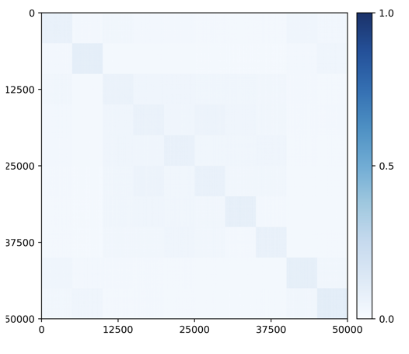
\includegraphics[width=0.5\textwidth]{\toplevelprefix/chapters/chapter5/figs/CIFAR10_cifar10_heatmap_zz.png}
    % }
    %  \subfigure[CIFAR-100]{
    %      \includegraphics[width=0.305\textwidth]{CIFAR100_cifar100_heatmap.png}
    %  }
    %  \subfigure[Tiny ImageNet]{
    %      \includegraphics[width=0.305\textwidth]{tinyimagenet_heatmap.png}
    %  }
    % \vspace{-0.15in}
    \caption{\small CIFAR-10 特征空间中 $|\Z^\top \Z|$ 的块对角结构的出现。}
    \label{fig:heatmap_z}
\end{figure}

\begin{figure}[h!]
    \begin{subfigure}[t]{0.46\textwidth}
        \centering
        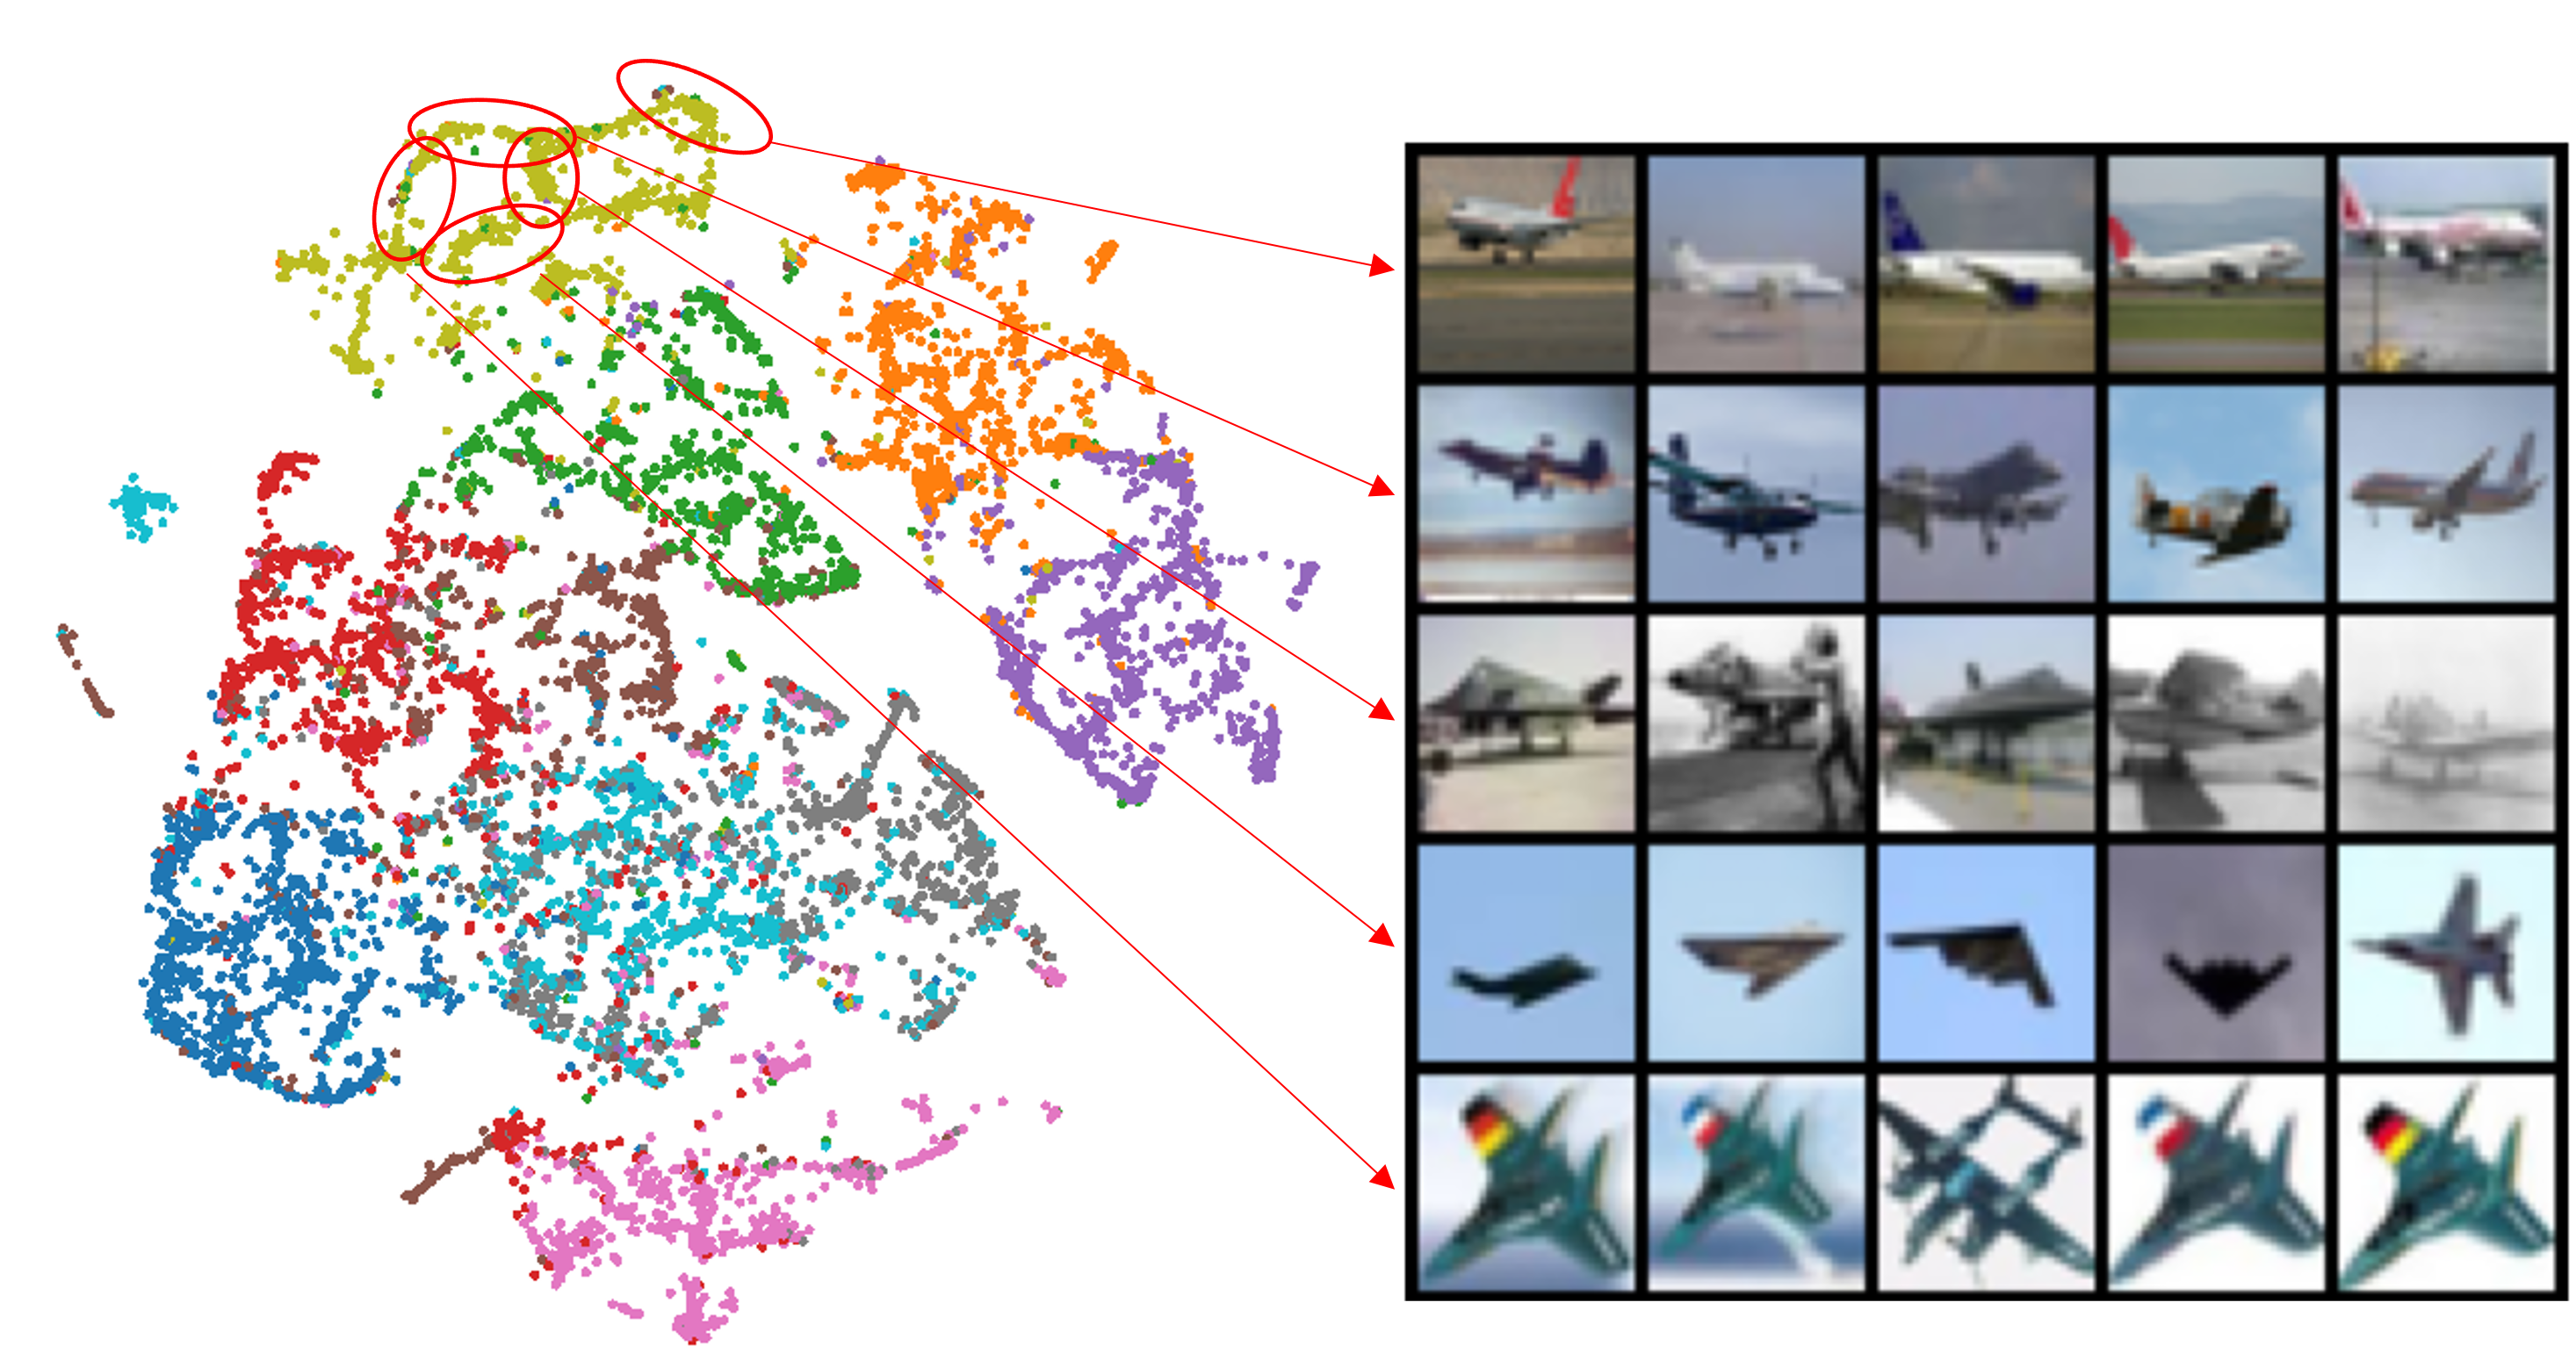
\includegraphics[width=\textwidth]{\toplevelprefix/chapters/chapter5/figs/uCTRL-tsne2.png}
        \caption{u-CTRL}
    \end{subfigure}
    \hfill
    \begin{subfigure}[t]{0.46\textwidth}
        \centering
        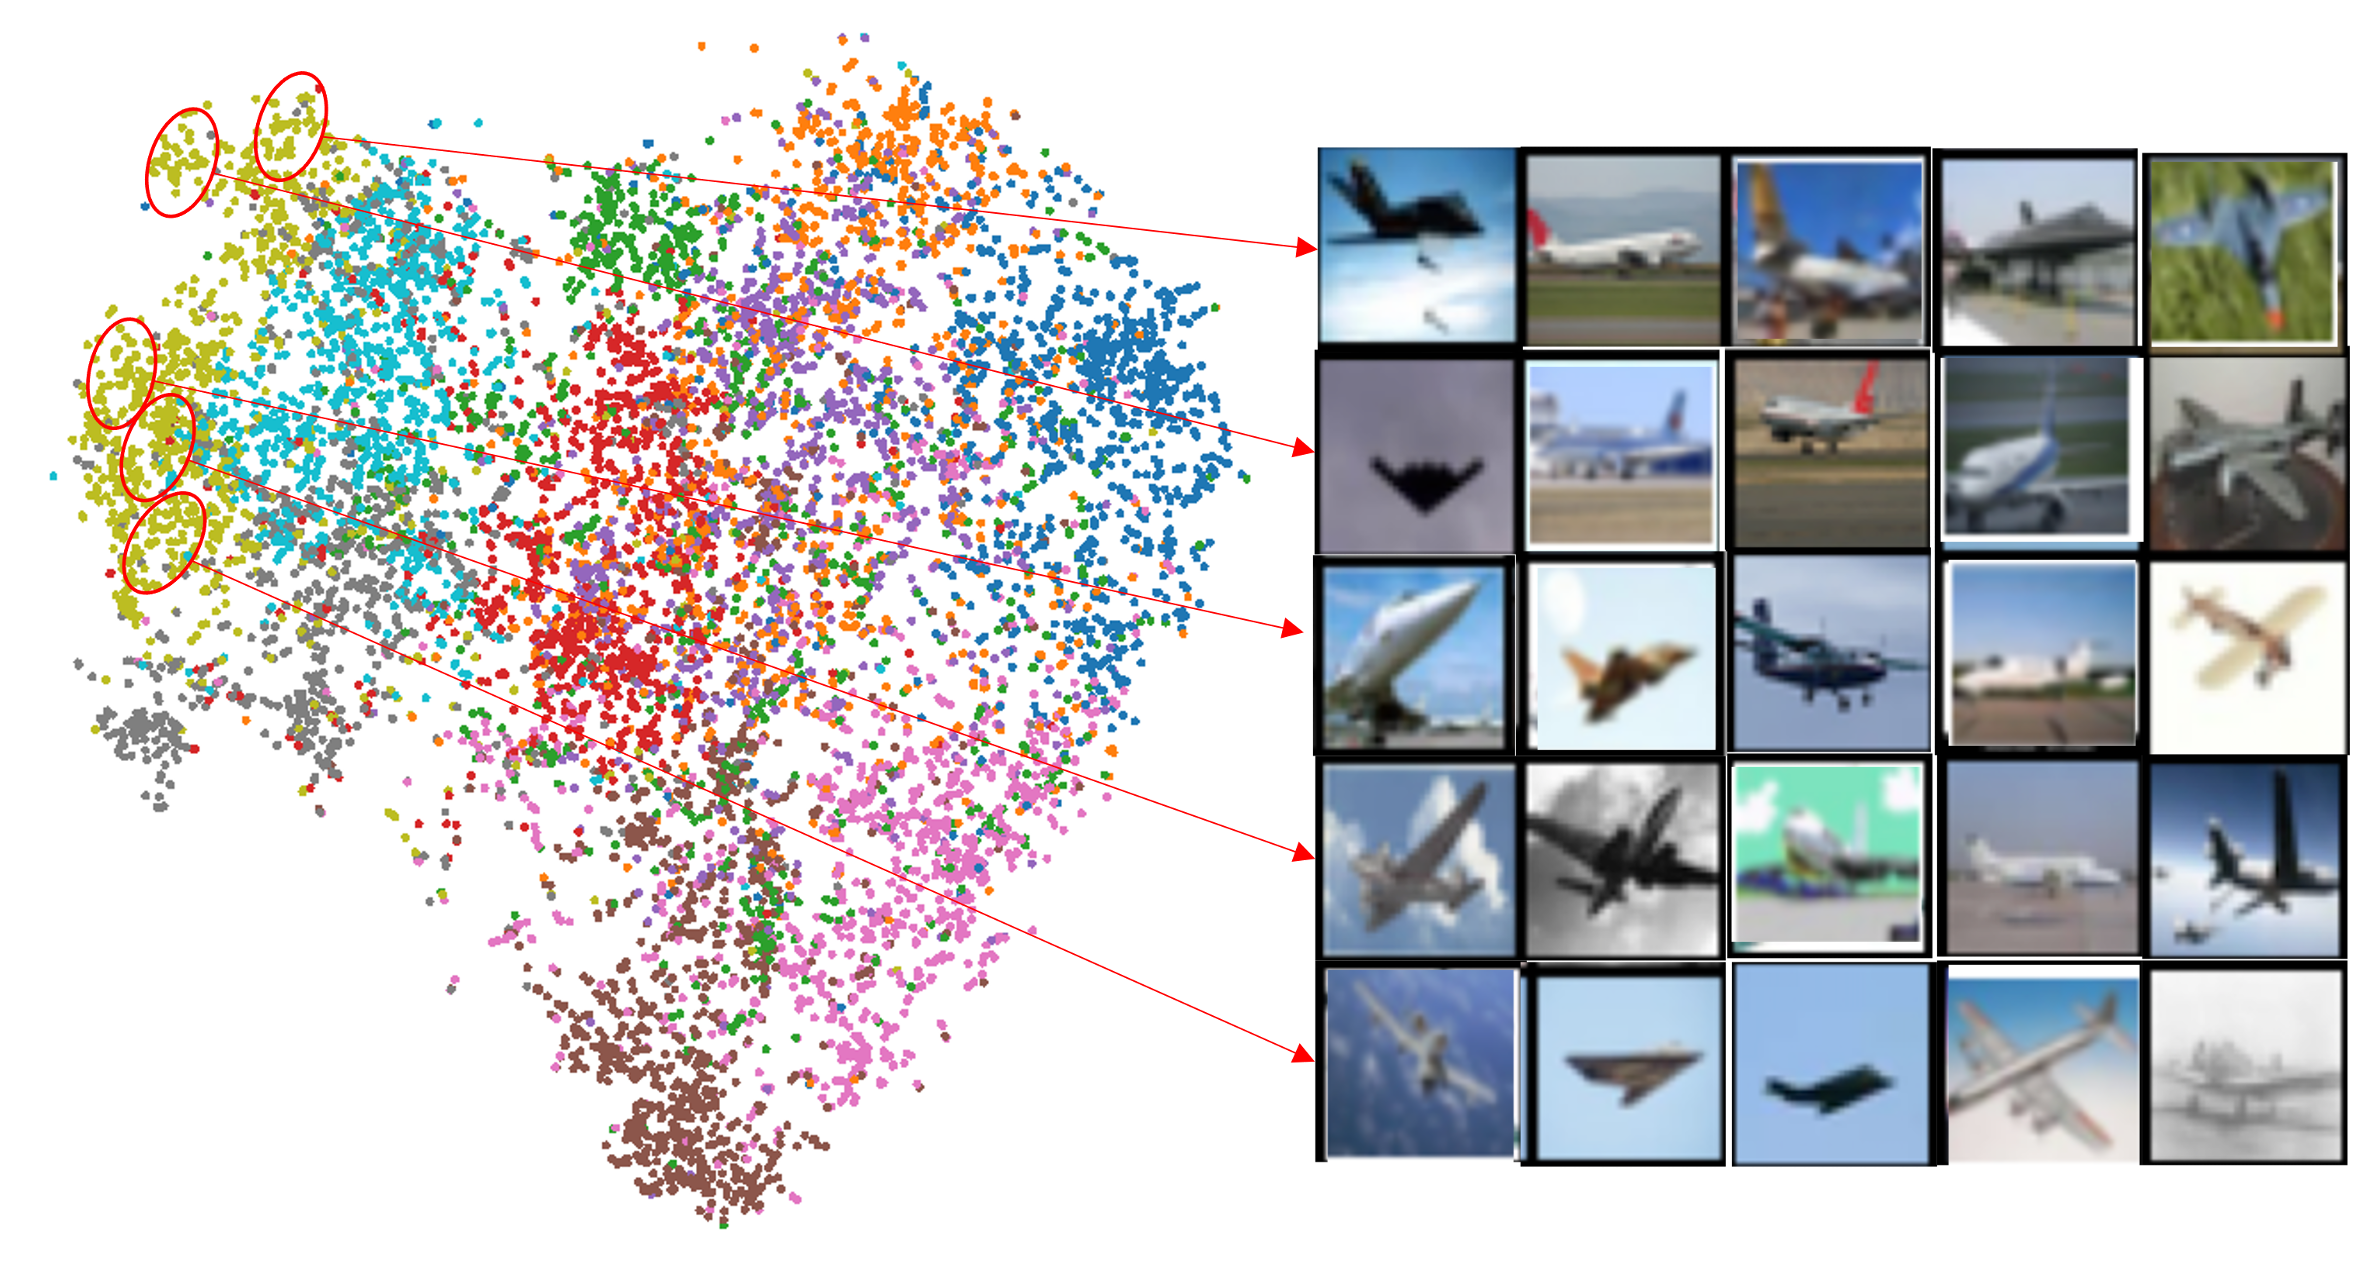
\includegraphics[width=\textwidth]{\toplevelprefix/chapters/chapter5/figs/MoCoV2-tsne3.png}
        \caption{MoCoV2}
    \end{subfigure}
    %  \footnotesize
    %  \centering
    %  \subfigure[u-CTRL]{
    %      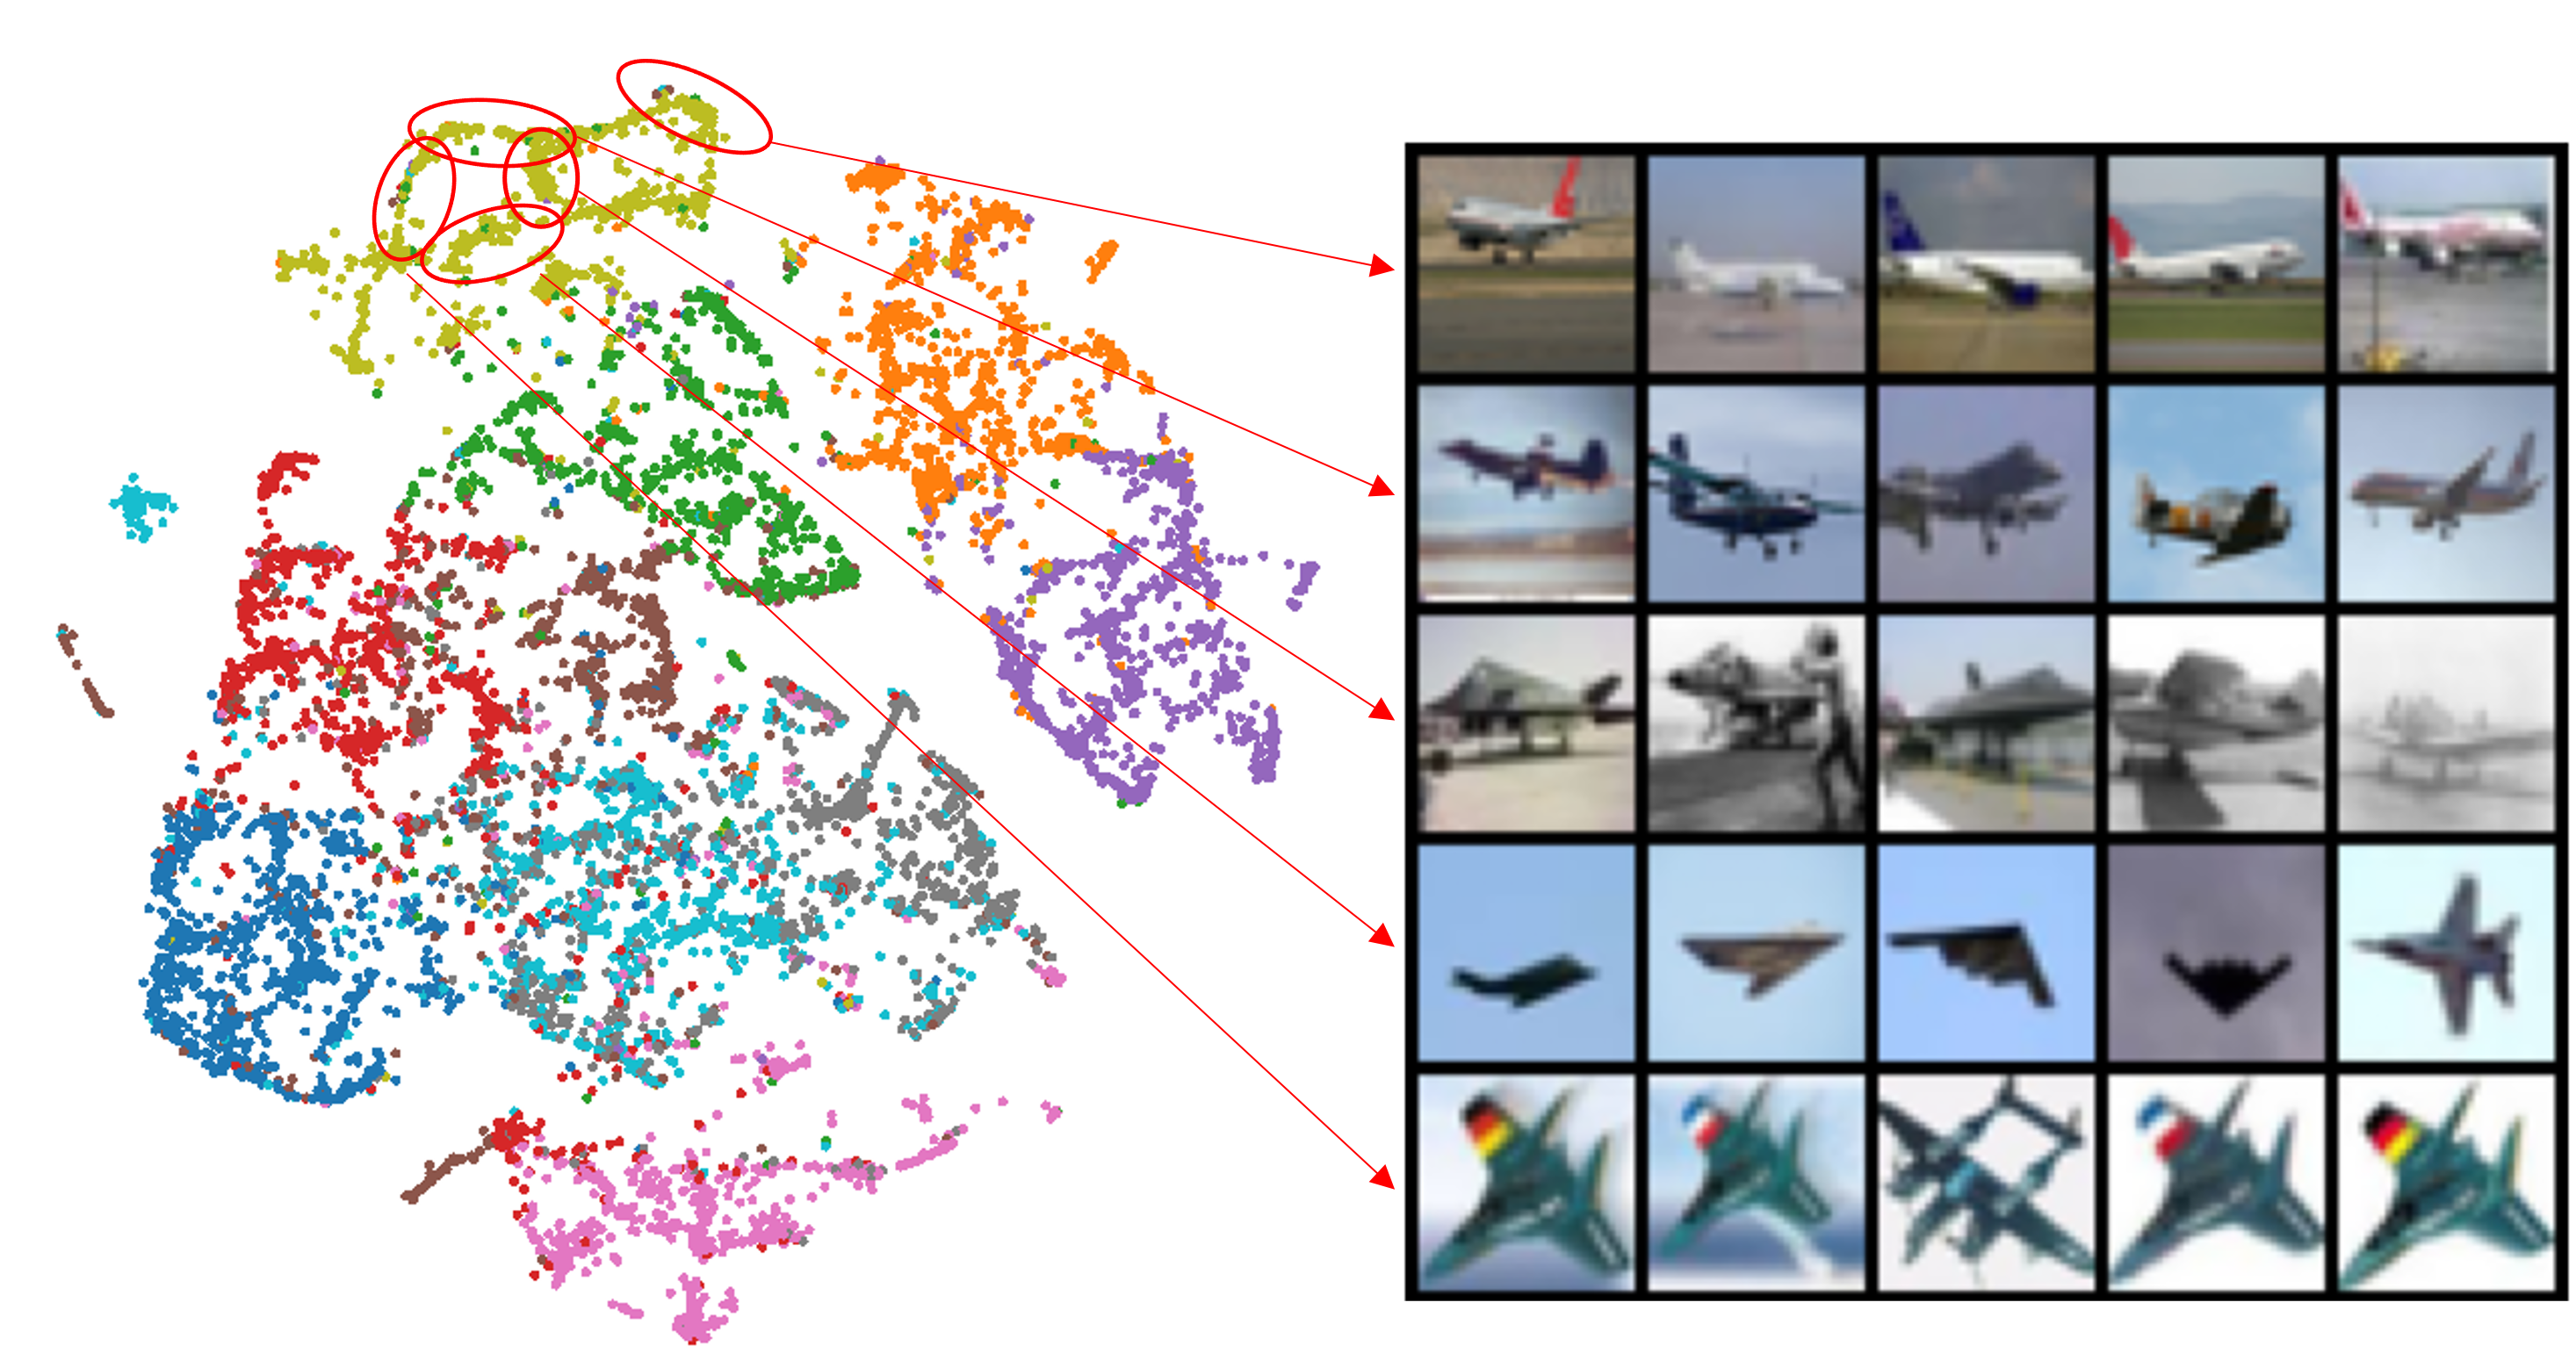
\includegraphics[width=0.46\textwidth]{\toplevelprefix/chapters/chapter5/figs/uCTRL-tsne2.png}
    %  }
    %  \subfigure[MoCoV2]{
    %      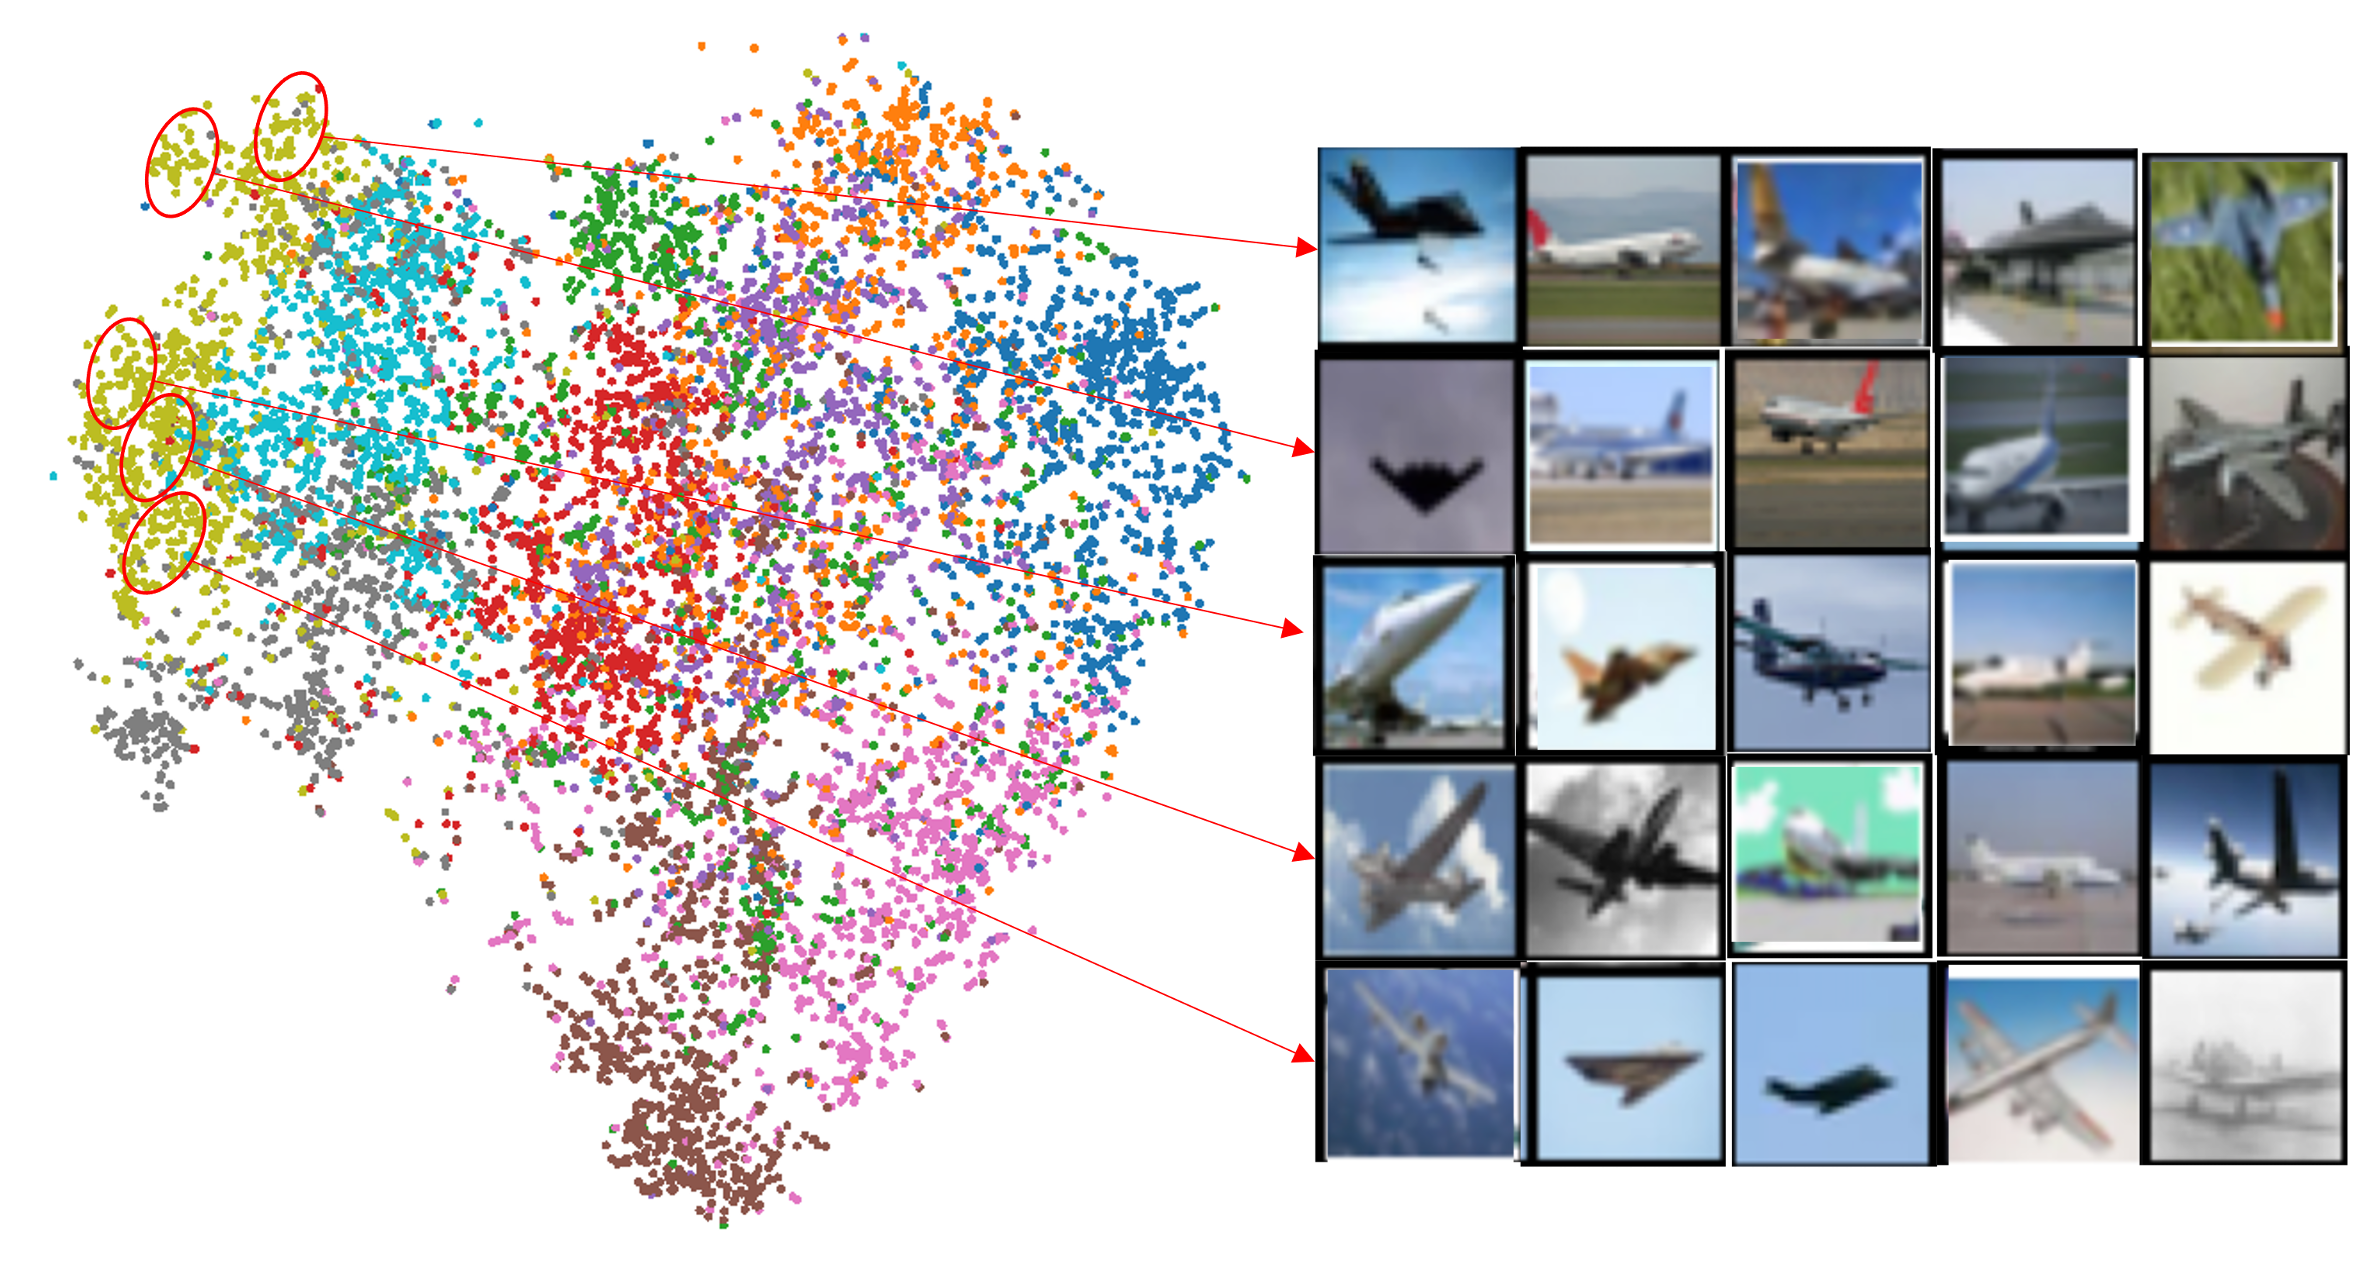
\includegraphics[width=0.46\textwidth]{\toplevelprefix/chapters/chapter5/figs/MoCoV2-tsne3.png}
    %  }
    \caption{\small 使用不同模型学习的 CIFAR-10 特征的 t-SNE 可视化。} 
    \label{fig:tsne}
\end{figure}

\paragraph{通过编码率降低进行无监督条件图像生成。}
高度结构化的特征分布也表明,学习到的表示对于生成目的非常有用。例如,我们可以将样本特征组织成有意义的簇,并用低维(高斯)分布或子空间对它们进行建模。通过从这些紧凑的模型中采样,我们可以有条件地从计算出的簇中重新生成有意义的样本。这被称为{\em 无监督条件图像生成} \cite{hwang2021stein}。

为了对特征进行聚类,我们利用了编码率降低框架 \eqref{eqn:maximal-rate-reduction} 的灵感来自于通过压缩进行无监督聚类 \cite{ma2007segmentation},这为找到成员关系 $\bm \Pi$ 提供了一种有原则的方法。
具体来说,我们最大化相同的编码率降低目标 \eqref{eqn:maximal-rate-reduction} over $\bm \Pi$,但固定学习到的表示 $\Z$。我们简单地将成员关系 $\bm \Pi$ 视为特征 $\Z$ 的一个非线性函数,比如 $h_{\bm \pi}(\cdot,\xi):\Z \mapsto \bm \Pi$,其参数为 $\xi$。在实践中,我们用一个简单的神经网络来建模这个函数,比如在输出特征 $\z$ 之后紧跟一个 MLP 头。
为了估计样本的“伪”成员关系 $\hat{\bm \Pi}$,我们解决以下关于 $\bm \Pi$ 的优化问题:
\begin{align}
    \hat{\bm \Pi} = \arg\max_{\xi} \Delta R(\Z| \bm \Pi(\xi)).
\label{eqn:cluster_mcr}
\end{align}
在图 \ref{fig:vis_clustering} 中,我们可视化了从 \eqref{eqn:cluster_mcr} 的十个无监督簇生成的图像。每个块代表一个簇,每一行代表每个簇的一个主成分。尽管在没有标签的情况下进行学习和训练,模型不仅能将样本组织成正确的簇,而且还能保留每个簇/类别内的统计多样性。我们可以通过计算不同的主成分,然后相应地进行采样和生成,轻松地恢复每个簇内的多样性。虽然这里展示的实验在规模上有些有限,但我们将在下一章中探索更直接、更强大的方法,利用学习到的数据分布和表示进行条件生成和估计。
\begin{figure}[t]
    \footnotesize
    \centering
    \includegraphics[width=0.95\textwidth]{\toplevelprefix/chapters/chapter5/figs/CIFAR10_generatedfromcluster.png}
    \caption{\small 使用 u-CTRL 从 CIFAR-10 的每个簇进行无监督条件图像生成。不同行的图像表示从每个簇的不同主成分生成。}
    \label{fig:vis_clustering}
\end{figure}




% \section{Other Variations} 
% to be determined...

\section{总结与注释}
本章介绍的材料基于一系列关于该主题的近期工作:\cite{Dai-entropy-2022}、
\cite{pai2022pursuit}、\cite{tong2023incremental} 和 \cite{pmlr-v234-tong24a}。特别是,第 \ref{sec:closed-loop-transcription} 节基于 \cite{Dai-entropy-2022} 的开创性工作。此后,\cite{pai2022pursuit} 的工作为闭环框架提供了强有力的理论论证,至少在一个理想情况下是这样。第 \ref{sec:class-wise-incremental} 节和第 \ref{sec:sample-wise-incremental} 节分别基于 \cite{tong2023incremental} 和 \cite{pmlr-v234-tong24a} 的工作。它们证明了闭环框架自然支持增量和持续学习,无论是在类别级还是样本级设置中。读者可以参考这些论文以获取更多的技术和实验细节。


\paragraph{浅层与深层神经网络,用于自编码及更多。}
在 \Cref{sub:nonlinear-pca} 中,我们讨论了 Cybenko 的通用逼近定理,以及它如何说明原则上一个具有单个隐藏层(和合适的逐元素非线性)的神经网络足以逼近任何足够规则的目标函数。当然,在实践中,神经网络在实践中占主导地位的主要架构原因是训练\textit{更深}神经网络技术的改进。
为什么深度是必要的?
从根本的角度来看,深度分离问题,即构造一个更深的神经网络可以比浅层网络以指数级更高的效率逼近给定目标函数类别的设置,
已经在理论文献中得到了广泛的研究:
例子包括 \cite{Telgarsky2016-sn,Bresler2020-xy,Venturi2021-qc}。
在实践中训练更深网络的容易性尚未从理论角度得到同样令人满意的答案。
ResNets \cite{he2016deep} 代表了使更深网络更容易训练的开创性实证工作,几乎在所有现代架构中都以某种形式使用。理论研究主要集中在非常深的网络的可训练性上,通过初始神经正切核 \cite{Buchanan2021-sj,Martens2021-cx} 进行量化,但这些研究并未对更深网络在训练中后期阶段的可训练性优势提供重要见解(但请参见 \cite{Yang2021-gw},这是一系列试图解决此问题的研究的根源)。

\section{练习与扩展}

\end{document}